% Customizable fields and text areas start with % >> below.
% Lines starting with the comment character (%) are normally removed before release outside the collaboration, but not those comments ending lines

% svn info. These are modified by svn at checkout time.
% The last version of these macros found before the maketitle will be the one on the front page,
% so only the main file is tracked.
% Do not edit by hand!
\RCS$Revision: 64557 $
\RCS$HeadURL: svn+ssh://svn.cern.ch/reps/tdr2/notes/EWK-11-011/trunk/EWK-11-011.tex $
\RCS$Id: EWK-11-011.tex 64557 2011-06-28 21:55:42Z tulika $
%%%%%%%%%%%%% ptdr definitions %%%%%%%%%%%%%%%%%%%%%
\def\Fileversion$#1: #2 ${\gdef\fileversion{#2}}
\def\Filedate$#1: #2-#3-#4 #5 ${\gdef\filedate{#2/#3/#4}}
\Fileversion$Revision: 227897 $
\Filedate$Date: 2014-02-16 08:24:34 -0600 (Sun, 16 Feb 2014) $
%%%%%%%%%%%%%%%%%%%%%%%%%%%%%%%%%%%%%%%%%%%%%%%%%%%%%%%%%%%%%%%%%%%%
%
%  CMS Common definitions style file
%
%  N.B. use of \newcommand rather than \newcommand means
%       that a definition is ignored if already specified
%
%                                              L. Taylor 18 Feb 2005
%%%%%%%%%%%%%%%%%%%%%%%%%%%%%%%%%%%%%%%%%%%%%%%%%%%%%%%%%%%%%%%%%%%%
\NeedsTeXFormat{LaTeX2e}
\ProvidesPackage{ptdr-definitions}[\filedate\space CMS Additional Macro Definitions (\fileversion)]
\RequirePackage{xspace}
\RequirePackage{amsmath}

% Some shorthand
% turn off italics
\newcommand {\etal}{\mbox{et al.}\xspace} %et al. - no preceding comma
\newcommand {\ie}{\mbox{i.e.}\xspace}     %i.e.
\newcommand {\eg}{\mbox{e.g.}\xspace}     %e.g.
\newcommand {\etc}{\mbox{etc.}\xspace}     %etc.
\newcommand {\vs}{\mbox{\sl vs.}\xspace}      %vs.
\newcommand {\mdash}{\ensuremath{\mathrm{-}}} % for use within formulas

% some terms whose definition we may change
\newcommand {\Lone}{Level-1\xspace} % Level-1 or L1 ?
\newcommand {\Ltwo}{Level-2\xspace}
\newcommand {\Lthree}{Level-3\xspace}

% Some software programs (alphabetized)
\newcommand{\ACERMC} {\textsc{AcerMC}\xspace}
\newcommand{\ALPGEN} {{\textsc{alpgen}}\xspace}
\newcommand{\CALCHEP} {{\textsc{CalcHEP}}\xspace}
\newcommand{\CHARYBDIS} {{\textsc{charybdis}}\xspace}
\newcommand{\CMKIN} {\textsc{cmkin}\xspace}
\newcommand{\CMSIM} {{\textsc{cmsim}}\xspace}
\newcommand{\CMSSW} {{\textsc{cmssw}}\xspace}
\newcommand{\COBRA} {{\textsc{cobra}}\xspace}
\newcommand{\COCOA} {{\textsc{cocoa}}\xspace}
\newcommand{\COMPHEP} {\textsc{CompHEP}\xspace}
\newcommand{\EVTGEN} {{\textsc{evtgen}}\xspace}
\newcommand{\FAMOS} {{\textsc{famos}}\xspace}
\newcommand{\GARCON} {\textsc{garcon}\xspace}
\newcommand{\GARFIELD} {{\textsc{garfield}}\xspace}
\newcommand{\GEANE} {{\textsc{geane}}\xspace}
\newcommand{\GEANTfour} {{\textsc{Geant4}}\xspace}
\newcommand{\GEANTthree} {{\textsc{geant3}}\xspace}
\newcommand{\GEANT} {{\textsc{geant}}\xspace}
\newcommand{\HDECAY} {\textsc{hdecay}\xspace}
\newcommand{\HERWIG} {{\textsc{herwig}}\xspace}
\newcommand{\HERWIGpp} {{\textsc{herwig++}}\xspace}
\newcommand{\POWHEG} {{\textsc{powheg}}\xspace}
\newcommand{\HIGLU} {{\textsc{higlu}}\xspace}
\newcommand{\HIJING} {{\textsc{hijing}}\xspace}
\newcommand{\IGUANA} {\textsc{iguana}\xspace}
\newcommand{\ISAJET} {{\textsc{isajet}}\xspace}
\newcommand{\ISAPYTHIA} {{\textsc{isapythia}}\xspace}
\newcommand{\ISASUGRA} {{\textsc{isasugra}}\xspace}
\newcommand{\ISASUSY} {{\textsc{isasusy}}\xspace}
\newcommand{\ISAWIG} {{\textsc{isawig}}\xspace}
\newcommand{\MADGRAPH} {\textsc{MadGraph}\xspace}
\newcommand{\MCATNLO} {\textsc{mc@nlo}\xspace}
\newcommand{\MCFM} {\textsc{mcfm}\xspace}
\newcommand{\MILLEPEDE} {{\textsc{millepede}}\xspace}
\newcommand{\ORCA} {{\textsc{orca}}\xspace}
\newcommand{\OSCAR} {{\textsc{oscar}}\xspace}
\newcommand{\PHOTOS} {\textsc{photos}\xspace}
\newcommand{\PROSPINO} {\textsc{prospino}\xspace}
\newcommand{\PYTHIA} {{\textsc{pythia}}\xspace}
\newcommand{\SHERPA} {{\textsc{sherpa}}\xspace}
\newcommand{\TAUOLA} {\textsc{tauola}\xspace}
\newcommand{\TOPREX} {\textsc{TopReX}\xspace}
\newcommand{\XDAQ} {{\textsc{xdaq}}\xspace}


%  Experiments
\newcommand {\DZERO}{D0\xspace}     %etc.


% Measurements and units...

\newcommand{\de}{\ensuremath{^\circ}}
\newcommand{\ten}[1]{\ensuremath{\times \text{10}^\text{#1}}}
\newcommand{\unit}[1]{\ensuremath{\text{\,#1}}\xspace}
\newcommand{\mum}{\ensuremath{\,\mu\text{m}}\xspace}
\newcommand{\micron}{\ensuremath{\,\mu\text{m}}\xspace}
\newcommand{\cm}{\ensuremath{\,\text{cm}}\xspace}
\newcommand{\mm}{\ensuremath{\,\text{mm}}\xspace}
\newcommand{\mus}{\ensuremath{\,\mu\text{s}}\xspace}
\newcommand{\keV}{\ensuremath{\,\text{ke\hspace{-.08em}V}}\xspace}
\newcommand{\MeV}{\ensuremath{\,\text{Me\hspace{-.08em}V}}\xspace}
\newcommand{\MeVns}{\ensuremath{\text{Me\hspace{-.08em}V}}\xspace} % no leading thinspace
\newcommand{\GeV}{\ensuremath{\,\text{Ge\hspace{-.08em}V}}\xspace}
\newcommand{\GeVns}{\ensuremath{\text{Ge\hspace{-.08em}V}}\xspace} % no leading thinspace
\newcommand{\gev}{\GeV}
\newcommand{\TeV}{\ensuremath{\,\text{Te\hspace{-.08em}V}}\xspace}
\newcommand{\TeVns}{\ensuremath{\text{Te\hspace{-.08em}V}}\xspace} % no leading thinspace
\newcommand{\PeV}{\ensuremath{\,\text{Pe\hspace{-.08em}V}}\xspace}
\newcommand{\keVc}{\ensuremath{{\,\text{ke\hspace{-.08em}V\hspace{-0.16em}/\hspace{-0.08em}}c}}\xspace}
\newcommand{\MeVc}{\ensuremath{{\,\text{Me\hspace{-.08em}V\hspace{-0.16em}/\hspace{-0.08em}}c}}\xspace}
\newcommand{\GeVc}{\ensuremath{{\,\text{Ge\hspace{-.08em}V\hspace{-0.16em}/\hspace{-0.08em}}c}}\xspace}
\newcommand{\GeVcns}{\ensuremath{{\text{Ge\hspace{-.08em}V\hspace{-0.16em}/\hspace{-0.08em}}c}}\xspace} % no leading thinspace
\newcommand{\TeVc}{\ensuremath{{\,\text{Te\hspace{-.08em}V\hspace{-0.16em}/\hspace{-0.08em}}c}}\xspace}
\newcommand{\keVcc}{\ensuremath{{\,\text{ke\hspace{-.08em}V\hspace{-0.16em}/\hspace{-0.08em}}c^\text{2}}}\xspace}
\newcommand{\MeVcc}{\ensuremath{{\,\text{Me\hspace{-.08em}V\hspace{-0.16em}/\hspace{-0.08em}}c^\text{2}}}\xspace}
\newcommand{\GeVcc}{\ensuremath{{\,\text{Ge\hspace{-.08em}V\hspace{-0.16em}/\hspace{-0.08em}}c^\text{2}}}\xspace}
\newcommand{\GeVccns}{\ensuremath{{\text{Ge\hspace{-.08em}V\hspace{-0.16em}/\hspace{-0.08em}}c^\text{2}}}\xspace} % no leading thinspace
\newcommand{\TeVcc}{\ensuremath{{\,\text{Te\hspace{-.08em}V\hspace{-0.16em}/\hspace{-0.08em}}c^\text{2}}}\xspace}

\newcommand{\pbinv} {\mbox{\ensuremath{\,\text{pb}^\text{$-$1}}}\xspace}
\newcommand{\fbinv} {\mbox{\ensuremath{\,\text{fb}^\text{$-$1}}}\xspace}
\newcommand{\nbinv} {\mbox{\ensuremath{\,\text{nb}^\text{$-$1}}}\xspace}
\newcommand{\mubinv} {\ensuremath{\,\mu\mathrm{b}^{-1}}\xspace}
\newcommand{\percms}{\ensuremath{\,\text{cm}^\text{$-$2}\,\text{s}^\text{$-$1}}\xspace}
\newcommand{\lumi}{\ensuremath{\mathcal{L}}\xspace}
\newcommand{\Lumi}{\ensuremath{\mathcal{L}}\xspace}%both upper and lower
%
% Need a convention here:
\newcommand{\LvLow}  {\ensuremath{\mathcal{L}=\text{10}^\text{32}\,\text{cm}^\text{$-$2}\,\text{s}^\text{$-$1}}\xspace}
\newcommand{\LLow}   {\ensuremath{\mathcal{L}=\text{10}^\text{33}\,\text{cm}^\text{$-$2}\,\text{s}^\text{$-$1}}\xspace}
\newcommand{\lowlumi}{\ensuremath{\mathcal{L}=\text{2}\times \text{10}^\text{33}\,\text{cm}^\text{$-$2}\,\text{s}^\text{$-$1}}\xspace}
\newcommand{\LMed}   {\ensuremath{\mathcal{L}=\text{2}\times \text{10}^\text{33}\,\text{cm}^\text{$-$2}\,\text{s}^\text{$-$1}}\xspace}
\newcommand{\LHigh}  {\ensuremath{\mathcal{L}=\text{10}^\text{34}\,\text{cm}^\text{$-$2}\,\text{s}^\text{$-$1}}\xspace}
\newcommand{\hilumi} {\ensuremath{\mathcal{L}=\text{10}^\text{34}\,\text{cm}^\text{$-$2}\,\text{s}^\text{$-$1}}\xspace}

% Physics symbols ...

\newcommand{\PT}{\ensuremath{p_{\mathrm{T}}}\xspace}
\newcommand{\pt}{\ensuremath{p_{\mathrm{T}}}\xspace}
\newcommand{\ET}{\ensuremath{E_{\mathrm{T}}}\xspace}
\newcommand{\HT}{\ensuremath{H_{\mathrm{T}}}\xspace}
\newcommand{\et}{\ensuremath{E_{\mathrm{T}}}\xspace}
\newcommand{\Em}{\ensuremath{E\hspace{-0.6em}/}\xspace}
\newcommand{\Pm}{\ensuremath{p\hspace{-0.5em}/}\xspace}
\newcommand{\PTm}{\ensuremath{{p}_\mathrm{T}\hspace{-1.02em}/\kern 0.5em}\xspace}
\newcommand{\PTslash}{\PTm}
\newcommand{\ETm}{\ensuremath{E_{\mathrm{T}}^{\text{miss}}}\xspace}
\newcommand{\MET}{\ETm}
\newcommand{\ETmiss}{\ETm}
\newcommand{\ETslash}{\ensuremath{E_{\mathrm{T}}\hspace{-1.1em}/\kern0.45em}\xspace}
\newcommand{\VEtmiss}{\ensuremath{{\vec E}_{\mathrm{T}}^{\text{miss}}}\xspace}
\newcommand{\ptvec}{\ensuremath{{\vec p}_{\mathrm{T}}}\xspace}

% roman face derivative
\newcommand{\dd}[2]{\ensuremath{\frac{\cmsSymbolFace{d} #1}{\cmsSymbolFace{d} #2}}}
\newcommand{\ddinline}[2]{\ensuremath{\cmsSymbolFace{d} #1/\cmsSymbolFace{d} #2}}
\newcommand{\rd}{\ensuremath{\cmsSymbolFace{d}}}
\newcommand{\re}{\ensuremath{\cmsSymbolFace{e}}}
% absolute value
\newcommand{\abs}[1]{\ensuremath{\lvert #1 \rvert}}



\ifthenelse{\boolean{cms@italic}}{\newcommand{\cmsSymbolFace}{\relax}}{\newcommand{\cmsSymbolFace}{\mathrm}}

% Particle names which track the italic/non-italic face convention
\newcommand{\zp}{\ensuremath{\cmsSymbolFace{Z}^\prime}\xspace} % plain Z'
\newcommand{\JPsi}{\ensuremath{\cmsSymbolFace{J}\hspace{-.08em}/\hspace{-.14em}\psi}\xspace} % J/Psi (no mass)
\newcommand{\Z}{\ensuremath{\cmsSymbolFace{Z}}\xspace} % plain Z (no superscript 0)
\newcommand{\ttbar}{\ensuremath{\cmsSymbolFace{t}\overline{\cmsSymbolFace{t}}}\xspace} % t-tbar

% Extensions for missing names in PENNAMES % note no xspace, to match syntax in PENNAMES
\newcommand{\cPgn}{\ensuremath{\nu}} % generic neutrino
\providecommand{\Pgn}{\ensuremath{\nu}} % generic neutrino
\newcommand{\cPagn}{\ensuremath{\overline{\nu}}} % generic neutrino
\providecommand{\Pagn}{\ensuremath{\overline{\nu}}} % generic neutrino
\newcommand{\cPgg}{\ensuremath{\gamma}} % gamma
\newcommand{\cPJgy}{\ensuremath{\cmsSymbolFace{J}\hspace{-.08em}/\hspace{-.14em}\psi}} % J/Psi (no mass)
\newcommand{\cPZ}{\ensuremath{\cmsSymbolFace{Z}}} % plain Z (no superscript 0)
\newcommand{\cPZpr}{\ensuremath{\cmsSymbolFace{Z}^\prime}} % plain Z'
\newcommand{\cPqt}{\ensuremath{\cmsSymbolFace{t}}} % t for t quark
\newcommand{\cPqb}{\ensuremath{\cmsSymbolFace{b}}} % b for b quark
\newcommand{\cPqc}{\ensuremath{\cmsSymbolFace{c}}} % c for c quark
\newcommand{\cPqs}{\ensuremath{\cmsSymbolFace{s}}} % s for s quark
\newcommand{\cPqu}{\ensuremath{\cmsSymbolFace{u}}} % u for u quark
\newcommand{\cPqd}{\ensuremath{\cmsSymbolFace{d}}} % d for d quark
\newcommand{\cPq}{\ensuremath{\cmsSymbolFace{q}}} % generic quark
\newcommand{\cPg}{\ensuremath{\cmsSymbolFace{g}}} % generic gluon
\newcommand{\cPG}{\ensuremath{\cmsSymbolFace{G}}} % Graviton
\newcommand{\cPaqt}{\ensuremath{\overline{\cmsSymbolFace{t}}}} % t for t anti-quark
\newcommand{\cPaqb}{\ensuremath{\overline{\cmsSymbolFace{b}}}} % b for b anti-quark
\newcommand{\cPaqc}{\ensuremath{\overline{\cmsSymbolFace{c}}}} % c for c anti-quark
\newcommand{\cPaqs}{\ensuremath{\overline{\cmsSymbolFace{s}}}} % s for s anti-quark
\newcommand{\cPaqu}{\ensuremath{\overline{\cmsSymbolFace{u}}}} % u for u anti-quark
\newcommand{\cPaqd}{\ensuremath{\overline{\cmsSymbolFace{d}}}} % d for d anti-quark
\newcommand{\cPaq}{\ensuremath{\overline{\cmsSymbolFace{q}}}} % generic anti-quark
\newcommand{\cPKstz}{\ensuremath{\cmsSymbolFace{K}^{\ast0}}\xspace} %note has xspace
% future symbols from heppennames2
\providecommand{\PH}{\ensuremath{\cmsSymbolFace{H}}\xspace} % plain Higgs
\providecommand{\PJGy}{\ensuremath{\cmsSymbolFace{J}\hspace{-.08em}/\hspace{-.14em}\psi}\xspace} % J/Psi (no mass)
\providecommand{\PBzs}{\ensuremath{\cmsSymbolFace{B}^0_\cmsSymbolFace{s}}\xspace} % B^0_s
\providecommand{\Pg}{\ensuremath{\cmsSymbolFace{g}}\xspace} % generic gluon
\providecommand{\PSg}{\ensuremath{\widetilde{\cmsSymbolFace{g}}}\xspace} % gluino
\providecommand{\PSQ}{\ensuremath{\widetilde{\cmsSymbolFace{q}}}\xspace} % squark
\providecommand{\PXXG}{\ensuremath{\cmsSymbolFace{G}}\xspace} % graviton
\providecommand{\PXXSG}{\ensuremath{\widetilde{\PXXG}}\xspace} % gravitino
\providecommand{\PSGcp}{\ensuremath{\widetilde{\chi}^+}\xspace}
\providecommand{\PSGc}{\ensuremath{\widetilde{\chi}}\xspace} % neutralino
\providecommand{\PSGcz}{\ensuremath{\widetilde{\chi}^0}\xspace} % neutralino with superscript 0
\providecommand{\PSGczDo}{\ensuremath{\widetilde{\chi}^{0}_{1}}\xspace} % neutralino
\providecommand{\PSGczDt}{\ensuremath{\widetilde{\chi}^{0}_{2}}\xspace} % neutralino
\providecommand{\PSGcpm}{\ensuremath{\widetilde{\chi}^\pm}\xspace} % neutralino
\providecommand{\Pl}{\ensuremath{\cmsSymbolFace{l}}\xspace} % non-ell lepton
\providecommand{\PAl}{\ensuremath{\overline{\cmsSymbolFace{l}}}\xspace} % non-ell anti-lepton
\providecommand{\PGnl}{\ensuremath{\nu_\cmsSymbolFace{l}}\xspace} % lepton neutrino
\providecommand{\PAGnl}{\ensuremath{\overline{\nu}_\cmsSymbolFace{l}}\xspace} % anti-lepton neutrino
\providecommand{\PQtpr}{\ensuremath{\cmsSymbolFace{t}^{\prime}}\xspace} % t'
\providecommand{\PAQtpr}{\ensuremath{\bar{\cmsSymbolFace{t}}^\prime}\xspace} % t'-bar; needs to be converted to overline-requires rework a la heppennames
\providecommand{\PQbpr}{\ensuremath{\cmsSymbolFace{b}^{\prime}}\xspace} % b'
\providecommand{\PAQbpr}{\ensuremath{\bar{\cmsSymbolFace{b}}^\prime}\xspace} % b'-bar; needs same as anti-t'
\providecommand{\PGg}{\ensuremath{\gamma}\xspace} % gamma
\providecommand{\PKzS}{\ensuremath{\cmsSymbolFace{K}^0_\cmsSymbolFace{S}}\xspace} % K short
\providecommand{\PBs}{\ensuremath{\cmsSymbolFace{B}_\cmsSymbolFace{s}}\xspace} % B sub s
\providecommand{\PSQt}{\ensuremath{\widetilde{\cmsSymbolFace{t}}}\xspace} % stop
\providecommand{\PZpr}{\ensuremath{\cmsSymbolFace{Z}^\prime}\xspace} % plain Z'
\providecommand{\PWpr}{\ensuremath{\cmsSymbolFace{W}^\prime}\xspace} % plain W'
\providecommand{\PGn}{\ensuremath{\nu}\xspace} % generic neutrino
\providecommand{\PAGn}{\ensuremath{\overline{\nu}}\xspace} % generic neutrino


% for APS style tables
\ifthenelse{\boolean{cms@external}}{%
\newenvironment{scotch}[1]{\protect\centering\ruledtabular\tabular{#1}}{\endtabular\endruledtabular}
}{
\newenvironment{scotch}[1]{\protect\centering\tabular{#1}\hline\hline}{\hline\endtabular}
}

% SM (still to be classified)

\newcommand{\AFB}{\ensuremath{A_\text{FB}}\xspace}
\newcommand{\wangle}{\ensuremath{\sin^{2}\theta_{\text{eff}}^\text{lept}(M^2_{\Z})}\xspace}
\newcommand{\stat}{\ensuremath{\,\text{(stat.)}}\xspace}
\newcommand{\syst}{\ensuremath{\,\text{(syst.)}}\xspace}
\newcommand{\lum}{\ensuremath{\,\text{(lum.)}}\xspace}
\newcommand{\kt}{\ensuremath{k_{\mathrm{T}}}\xspace}

\newcommand{\BC}{\ensuremath{\cmsSymbolFace{B_{c}}}\xspace}
\newcommand{\bbarc}{\ensuremath{\cPqb\cPaqc}\xspace}
\newcommand{\bbbar}{\ensuremath{\cPqb\cPaqb}\xspace}
\newcommand{\ccbar}{\ensuremath{\cPqc\cPaqc}\xspace}
\newcommand{\bspsiphi}{\ensuremath{\cmsSymbolFace{B_s} \to \JPsi\, \phi}\xspace}
\newcommand{\EE}{\ensuremath{\Pep\Pem}\xspace}
\newcommand{\MM}{\ensuremath{\Pgmp\Pgmm}\xspace}
\newcommand{\TT}{\ensuremath{\Pgt^{+}\Pgt^{-}}\xspace}

%%%  E-gamma definitions
\newcommand{\HGG}{\ensuremath{\cmsSymbolFace{H}\to\gamma\gamma}}
\newcommand{\GAMJET}{\ensuremath{\gamma + \text{jet}}}
\newcommand{\PPTOJETS}{\ensuremath{\Pp\Pp\to\text{jets}}}
\newcommand{\PPTOGG}{\ensuremath{\Pp\Pp\to\gamma\gamma}}
\newcommand{\PPTOGAMJET}{\ensuremath{\Pp\Pp\to\gamma + \mathrm{jet}}}
\newcommand{\MH}{\ensuremath{M_{\PH}}}
\newcommand{\RNINE}{\ensuremath{R_\mathrm{9}}}
\newcommand{\DR}{\ensuremath{\Delta R}}





%%%%%%
% From Albert
%

\newcommand{\ga}{\ensuremath{\gtrsim}}
\newcommand{\la}{\ensuremath{\lesssim}}
%
\newcommand{\swsq}{\ensuremath{\sin^2\theta_\cmsSymbolFace{W}}\xspace}
\newcommand{\cwsq}{\ensuremath{\cos^2\theta_\cmsSymbolFace{W}}\xspace}
\newcommand{\tanb}{\ensuremath{\tan\beta}\xspace}
\newcommand{\tanbsq}{\ensuremath{\tan^{2}\beta}\xspace}
\newcommand{\sidb}{\ensuremath{\sin 2\beta}\xspace}
\newcommand{\alpS}{\ensuremath{\alpha_S}\xspace}
\newcommand{\alpt}{\ensuremath{\tilde{\alpha}}\xspace}

\newcommand{\QL}{\ensuremath{\cmsSymbolFace{Q}_\cmsSymbolFace{L}}\xspace}
\newcommand{\sQ}{\ensuremath{\widetilde{\cmsSymbolFace{Q}}}\xspace}
\newcommand{\sQL}{\ensuremath{\widetilde{\cmsSymbolFace{Q}}_\cmsSymbolFace{L}}\xspace}
\newcommand{\ULC}{\ensuremath{\cmsSymbolFace{U}_\cmsSymbolFace{L}^\cmsSymbolFace{C}}\xspace}
\newcommand{\sUC}{\ensuremath{\widetilde{\cmsSymbolFace{U}}^\cmsSymbolFace{C}}\xspace}
\newcommand{\sULC}{\ensuremath{\widetilde{\cmsSymbolFace{U}}_\cmsSymbolFace{L}^\cmsSymbolFace{C}}\xspace}
\newcommand{\DLC}{\ensuremath{\cmsSymbolFace{D}_\cmsSymbolFace{L}^\cmsSymbolFace{C}}\xspace}
\newcommand{\sDC}{\ensuremath{\widetilde{\cmsSymbolFace{D}}^\cmsSymbolFace{C}}\xspace}
\newcommand{\sDLC}{\ensuremath{\widetilde{\cmsSymbolFace{D}}_\cmsSymbolFace{L}^\cmsSymbolFace{C}}\xspace}
\newcommand{\LL}{\ensuremath{\cmsSymbolFace{L}_\cmsSymbolFace{L}}\xspace}
\newcommand{\sL}{\ensuremath{\widetilde{\cmsSymbolFace{L}}}\xspace}
\newcommand{\sLL}{\ensuremath{\widetilde{\cmsSymbolFace{L}}_\cmsSymbolFace{L}}\xspace}
\newcommand{\ELC}{\ensuremath{\cmsSymbolFace{E}_\cmsSymbolFace{L}^\cmsSymbolFace{C}}\xspace}
\newcommand{\sEC}{\ensuremath{\widetilde{\cmsSymbolFace{E}}^\cmsSymbolFace{C}}\xspace}
\newcommand{\sELC}{\ensuremath{\widetilde{\cmsSymbolFace{E}}_\cmsSymbolFace{L}^\cmsSymbolFace{C}}\xspace}
\newcommand{\sEL}{\ensuremath{\widetilde{\cmsSymbolFace{E}}_\cmsSymbolFace{L}}\xspace}
\newcommand{\sER}{\ensuremath{\widetilde{\cmsSymbolFace{E}}_\cmsSymbolFace{R}}\xspace}
\newcommand{\sFer}{\ensuremath{\widetilde{\cmsSymbolFace{f}}}\xspace}
\newcommand{\sQua}{\ensuremath{\widetilde{\cmsSymbolFace{q}}}\xspace}
\newcommand{\sUp}{\ensuremath{\widetilde{\cmsSymbolFace{u}}}\xspace}
\newcommand{\suL}{\ensuremath{\widetilde{\cmsSymbolFace{u}}_\cmsSymbolFace{L}}\xspace}
\newcommand{\suR}{\ensuremath{\widetilde{\cmsSymbolFace{u}}_\cmsSymbolFace{R}}\xspace}
\newcommand{\sDw}{\ensuremath{\widetilde{\cmsSymbolFace{d}}}\xspace}
\newcommand{\sdL}{\ensuremath{\widetilde{\cmsSymbolFace{d}}_\cmsSymbolFace{L}}\xspace}
\newcommand{\sdR}{\ensuremath{\widetilde{\cmsSymbolFace{d}}_\cmsSymbolFace{R}}\xspace}
\newcommand{\sTop}{\ensuremath{\widetilde{\cmsSymbolFace{t}}}\xspace}
\newcommand{\stL}{\ensuremath{\widetilde{\cmsSymbolFace{t}}_\cmsSymbolFace{L}}\xspace}
\newcommand{\stR}{\ensuremath{\widetilde{\cmsSymbolFace{t}}_\cmsSymbolFace{R}}\xspace}
\newcommand{\stone}{\ensuremath{\widetilde{\cmsSymbolFace{t}}_1}\xspace}
\newcommand{\sttwo}{\ensuremath{\widetilde{\cmsSymbolFace{t}}_2}\xspace}
\newcommand{\sBot}{\ensuremath{\widetilde{\cmsSymbolFace{b}}}\xspace}
\newcommand{\sbL}{\ensuremath{\widetilde{\cmsSymbolFace{b}}_\cmsSymbolFace{L}}\xspace}
\newcommand{\sbR}{\ensuremath{\widetilde{\cmsSymbolFace{b}}_\cmsSymbolFace{R}}\xspace}
\newcommand{\sbone}{\ensuremath{\widetilde{\cmsSymbolFace{b}}_1}\xspace}
\newcommand{\sbtwo}{\ensuremath{\widetilde{\cmsSymbolFace{b}}_2}\xspace}
\newcommand{\sLep}{\ensuremath{\widetilde{\cmsSymbolFace{l}}}\xspace}
\newcommand{\sLepC}{\ensuremath{\widetilde{\cmsSymbolFace{l}}^\cmsSymbolFace{C}}\xspace}
\newcommand{\sEl}{\ensuremath{\widetilde{\cmsSymbolFace{e}}}\xspace}
\newcommand{\sElC}{\ensuremath{\widetilde{\cmsSymbolFace{e}}^\cmsSymbolFace{C}}\xspace}
\newcommand{\seL}{\ensuremath{\widetilde{\cmsSymbolFace{e}}_\cmsSymbolFace{L}}\xspace}
\newcommand{\seR}{\ensuremath{\widetilde{\cmsSymbolFace{e}}_\cmsSymbolFace{R}}\xspace}
\newcommand{\snL}{\ensuremath{\widetilde{\nu}_L}\xspace}
\newcommand{\sMu}{\ensuremath{\widetilde{\mu}}\xspace}
\newcommand{\sNu}{\ensuremath{\widetilde{\nu}}\xspace}
\newcommand{\sTau}{\ensuremath{\widetilde{\tau}}\xspace}
\newcommand{\Glu}{\ensuremath{\cmsSymbolFace{g}}\xspace}
\newcommand{\sGlu}{\ensuremath{\widetilde{\cmsSymbolFace{g}}}\xspace}
\newcommand{\Wpm}{\ensuremath{\cmsSymbolFace{W}^{\pm}}\xspace}
\newcommand{\sWpm}{\ensuremath{\widetilde{\cmsSymbolFace{W}}^{\pm}}\xspace}
\newcommand{\Wz}{\ensuremath{\cmsSymbolFace{W}^{0}}\xspace}
\newcommand{\sWz}{\ensuremath{\widetilde{\cmsSymbolFace{W}}^{0}}\xspace}
\newcommand{\sWino}{\ensuremath{\widetilde{\cmsSymbolFace{W}}}\xspace}
\newcommand{\Bz}{\ensuremath{\cmsSymbolFace{B}^{0}}\xspace}
\newcommand{\sBz}{\ensuremath{\widetilde{\cmsSymbolFace{B}}^{0}}\xspace}
\newcommand{\sBino}{\ensuremath{\widetilde{\cmsSymbolFace{B}}}\xspace}
\newcommand{\Zz}{\ensuremath{\cmsSymbolFace{Z}^{0}}\xspace}
\newcommand{\sZino}{\ensuremath{\widetilde{\cmsSymbolFace{Z}}^{0}}\xspace}
\newcommand{\sGam}{\ensuremath{\widetilde{\gamma}}\xspace}
\newcommand{\chiz}{\ensuremath{\widetilde{\chi}^{0}}\xspace}
\newcommand{\chip}{\ensuremath{\widetilde{\chi}^{+}}\xspace}
\newcommand{\chim}{\ensuremath{\widetilde{\chi}^{-}}\xspace}
\newcommand{\chipm}{\ensuremath{\widetilde{\chi}^{\pm}}\xspace}
\newcommand{\Hone}{\ensuremath{\cmsSymbolFace{H}_\cmsSymbolFace{d}}\xspace}
\newcommand{\sHone}{\ensuremath{\widetilde{\cmsSymbolFace{H}}_\cmsSymbolFace{d}}\xspace}
\newcommand{\Htwo}{\ensuremath{\cmsSymbolFace{H}_\cmsSymbolFace{u}}\xspace}
\newcommand{\sHtwo}{\ensuremath{\widetilde{\cmsSymbolFace{H}}_\cmsSymbolFace{u}}\xspace}
\newcommand{\sHig}{\ensuremath{\widetilde{\cmsSymbolFace{H}}}\xspace}
\newcommand{\sHa}{\ensuremath{\widetilde{\cmsSymbolFace{H}}_\cmsSymbolFace{a}}\xspace}
\newcommand{\sHb}{\ensuremath{\widetilde{\cmsSymbolFace{H}}_\cmsSymbolFace{b}}\xspace}
\newcommand{\sHpm}{\ensuremath{\widetilde{\cmsSymbolFace{H}}^{\pm}}\xspace}
\newcommand{\hz}{\ensuremath{\cmsSymbolFace{h}^{0}}\xspace}
\newcommand{\Hz}{\ensuremath{\cmsSymbolFace{H}^{0}}\xspace}
\newcommand{\Az}{\ensuremath{\cmsSymbolFace{A}^{0}}\xspace}
\newcommand{\Hpm}{\ensuremath{\cmsSymbolFace{H}^{\pm}}\xspace}
\newcommand{\sGra}{\ensuremath{\widetilde{\cmsSymbolFace{G}}}\xspace}
%
\newcommand{\mtil}{\ensuremath{\widetilde{m}}\xspace}
%
\newcommand{\rpv}{\ensuremath{\rlap{\kern.2em/}R}\xspace}
\newcommand{\LLE}{\ensuremath{LL\bar{E}}\xspace}
\newcommand{\LQD}{\ensuremath{LQ\bar{D}}\xspace}
\newcommand{\UDD}{\ensuremath{\overline{UDD}}\xspace}
\newcommand{\Lam}{\ensuremath{\lambda}\xspace}
\newcommand{\Lamp}{\ensuremath{\lambda'}\xspace}
\newcommand{\Lampp}{\ensuremath{\lambda''}\xspace}
%
\newcommand{\spinbd}[2]{\ensuremath{\bar{#1}_{\dot{#2}}}\xspace}

\newcommand{\MD}{\ensuremath{{M_\mathrm{D}}}\xspace}% ED mass
\newcommand{\Mpl}{\ensuremath{{M_\mathrm{Pl}}}\xspace}% Planck mass
\newcommand{\Rinv} {\ensuremath{{R}^{-1}}\xspace}
\endinput
 %These have been replaced by the equivalent style file
%%%%%%%%%%%%%%%  Additional definitions %%%%%%%%%%%%%%%%%%%%%%%%
\newcommand{\comment}[1]{}
\newcommand{\pb}{\ensuremath{\mathrm{pb}}}%
\newcommand{\pp}{\ensuremath{\mathrm{pp}}}%
\newcommand{\Wo}{\ensuremath{\mathrm{W}}}%
\newcommand{\Wp}{\ensuremath{\mathrm{W^+}}}%
\newcommand{\Wm}{\ensuremath{\mathrm{W^-}}}%
\newcommand{\Zo}{\ensuremath{\mathrm{Z}}}%
\newcommand{\rts}{\ensuremath{\sqrt{s}}}%
\newcommand{\ra}{\ensuremath{\rightarrow}}%
\newcommand{\MW}{\ensuremath{\mathrm{m}_\Wo}}%
\newcommand{\MZ}{\ensuremath{\mathrm{m}_\Zo}}%
\newcommand{\MT}{\ensuremath{\mathrm{M}_T}}%
\newcommand{\MLL}{\ensuremath{\mathrm{M}_{\ell\ell}}}%
\newcommand{\met}{\ensuremath{{E\!\!\!/}_{\mathrm{T}}}\xspace}
\renewcommand{\ttbar}{\ensuremath{\mathrm{t}\bar{\mathrm{t}}}}%
\newcommand{\Wmn}{\ensuremath{\Wo \ra \MN}}%
\newcommand{\Wpmn}{\ensuremath{\Wp \ra \mu^+\nu}}%
\newcommand{\Wmmn}{\ensuremath{\Wm \ra \mu^-\overline{\nu}}}%
\newcommand{\Zmm}{\ensuremath{\Zo \ra \MM}}%
\newcommand{\Wtn}{\ensuremath{\Wo \ra \tau\nu}}%
\newcommand{\Ztt}{\ensuremath{\Zo \ra \tau^+\tau^-}}%
\newcommand{\Wen}{\ensuremath{\Wo \ra \EN}}%
\newcommand{\Wpen}{\ensuremath{\Wp \ra \mathrm{e}^+\nu}}%
\newcommand{\Wmen}{\ensuremath{\Wm \ra \mathrm{e}^-\overline{\nu}}}%
\newcommand{\Zee}{\ensuremath{\Zo \ra \EE}}%
\newcommand{\Zll}{\ensuremath{\Zo \ra \ell^+ \ell^-}}%
\newcommand{\Wev}{\Wen}
\newcommand{\Wmv}{\Wmn}
\newcommand{\Ztautau}{\Ztt}
\renewcommand{\MET}{\met}
\newcommand{\invpb}{\mbox{$\textrm{pb}^{-1}$}}
\newcommand{\pth}{\hat{p}_{\perp}}
\newcommand{\Pt}{p_{T}}
\newcommand{\Et}{E_{T}}
\newcommand{\Lint}{\ensuremath{{\cal L}_{\mathrm{int}}}}
\newcommand{\IRelComb} {I^{\textrm{rel}}_{\textrm{comb}}}%
\newcommand{\Nbg}{N_{\mathrm{bg}}}%
\newcommand{\mumu}{\mu\mu}
\newcommand{\Zmumu}{Z_{\mumu}}
\newcommand{\Zmus}{Z_{\mu s}}
\newcommand{\Zmut}{Z_{\mu t}}
\newcommand{\nonIso}{\mathrm{non\,iso}}
\newcommand{\Wln}{W \rightarrow \ell \nu} 
% GHM
\def\ERROR#1#2{ \ensuremath{ \pm #1\, (\textrm{#2}) } \xspace }
\def\RESA#1#2#3{ \ensuremath{ #1 \ERROR{#2}{#3} } \xspace}
\def\RESB#1#2#3#4#5{ \ensuremath{ \RESA{#1}{#2}{#3} \ERROR{#4}{#5} } \xspace}
\def\RESC#1#2#3#4#5#6#7{ \ensuremath{ \RESB{#1}{#2}{#3}{#4}{#5} \ERROR{#6}{#7} } \xspace}
\def\RESD#1#2{ \ensuremath{ #1 \pm #2 } }
\def\RESE#1#2#3#4#5#6#7#8#9{ \ensuremath{ \RESC{#1}{#2}{#3}{#4}{#5}{#6}{#7} \ERROR{#8}{#9} } \xspace}
\def\RESGD#1#2#3#4{ \ensuremath{ \RESC{#1}{#2}{stat.}{#3}{syst.}{#4}{lumi.} }}
\def\EFF#1#2{ \ensuremath{ (\RESA{#1}{#2}{stat.})\% } \xspace}
\def\EFFA#1#2{ \ensuremath{ ({#1} \pm {#2})\% } \xspace}
\def\EFFB#1#2#3{ \ensuremath{ (\RESA{#1}{#2}{stat.} \ERROR{#3}{syst.})\% } \xspace}
%\def\EFFA#1#2{ \ensuremath{ \PRINTEFF{#1}{#2} } \xspace}
\def\SIGBR#1#2{  \ensuremath{ \sigma \left( \pp \to #1 X \right) \times {\cal B} \left( #1 \to #2 \right) } \xspace}
\def\SIGBRSHORT#1{\ensuremath{ \sigma\times{\cal B}(#1) }}
\def\RESSIGBR#1#2#3#4#5#6{  \ensuremath{ \SIGBR{#1}{#2} &=& \RESC{#3}{#4}{stat.}{#5}{syst.}{#6}{lumi.} \, \textrm{nb} } \xspace}
\def\RESSIGBRTH#1#2#3#4#5#6#7{  \ensuremath{ \SIGBR{#1}{#2} &=& \RESE{#3}{#4}{stat.}{#5}{syst.}{#6}{th.}{#7}{lumi.} \, \textrm{nb} } \xspace}
\def\RATWZ#1#2{ \ensuremath{ {
 \frac{ \sigma(\pp\rightarrow \Wo X)\times {\cal B}(\Wo\rightarrow #1)  }
      { \sigma(\pp\rightarrow \Zo X)\times {\cal B}(\Zo\rightarrow #2)  }   }  } }
\def\RESRATWZ#1#2#3#4#5#6{ \ensuremath{ \RATWZ{#1}{#2} &=& 
                                   #3 \ERROR{#4}{stat.} \ERROR{#5}{syst.} \ERROR{#6}{th.}} }
\def\RATWW#1#2{ \ensuremath{ {
 \frac{ \sigma(\pp\rightarrow \Wp X)\times {\cal B}(\Wp\rightarrow #1)  }
      { \sigma(\pp\rightarrow \Wm X)\times {\cal B}(\Wm\rightarrow #2)  }   }  } }
\def\RESRATWW#1#2#3#4#5#6{ \ensuremath{ \RATWW{#1}{#2} &=& 
                                   #3 \ERROR{#4}{stat.} \ERROR{#5}{syst.} \ERROR{#6}{th.}} }

\def\THEORYSIGBR#1#2{\ensuremath{ \RESD{#1}{#2}~{\mathrm{nb}} }}
\def\THEORYRATIO#1#2{\ensuremath{ \RESD{#1}{#2} }}

\def\EPS#1{ \ensuremath{ \epsilon_{\textrm{#1}} } \xspace}
\def\EPSTNPALL#1{ \ensuremath{ \EPS{\tnp-WP{#1}-ALL}  } \xspace }
\def\EPSTNPREC{ \ensuremath{ \EPS{\tnp-rec} } \xspace }
\def\EPSTNPTRG{ \ensuremath{ \EPS{\tnp-trg} } \xspace }
\def\EPSTNPWP#1{ \ensuremath{ \EPS{\tnp-WP{#1} } } \xspace }
\def\EPSTNPTRGWP#1{ \ensuremath{ \EPS{\tnp-TRG{#1}} } \xspace }  % MHS

% integrated luminosity
\newcommand{\THELUMI} {\ensuremath{{35.9\pm 1.4}~\mathrm{pb}^{-1}}}%

% Tag'n probe efficiencies 

% I=Inclusive; P=Plus; M=Minus

% WPW = Working Point @ 80\%  -- WPZ = Working Point @ 95\%

% one bin
\def\WPWIEFFRECO{   \ensuremath{\EFFA{99.7}{1.0}} \xspace} % GHM
\def\WPWIEFFID{     \ensuremath{\EFFA{76.3}{1.9}} \xspace} % GHM
\def\WPWIEFFHLT{    \ensuremath{\EFFA{98.9}{1.3}} \xspace} % GHM
\def\WPWIEFF{       \ensuremath{\EFFA{75.3}{2.3}} \xspace} % GHM 
\def\WPWIEFFMC{     \ensuremath{ 79.98\% } \xspace} % GHM
\def\WPWITNPR{      \ensuremath{\RESD{0.941}{0.028}} \xspace}  % !!!

% EB
\def\WPWIEBEFFRECO{   \ensuremath{\EFFA{97.0}{1.0}} \xspace} % GHM 
\def\WPWIEBMCRECO{   \ensuremath{\EFFA{97.78}{0.02}} \xspace}  % GHM
\def\WPWIEBRRECO{   \ensuremath{\RESD{0.992}{0.011}} \xspace} % GHM

\def\WPWIEBEFFID{   \ensuremath{\EFFA{84.0}{0.3}} \xspace} %GHM 
\def\WPWIEBMCID{   \ensuremath{\EFFA{87.47}{0.05}} \xspace} % GHM
\def\WPWIEBRID{   \ensuremath{\RESD{0.960}{0.004}} \xspace} % GHM

\def\WPZIEBEFFID{   \ensuremath{\EFFA{93.9}{1.5}} \xspace} % GHM
\def\WPZIEBMCID{   \ensuremath{ 96.4\% } \xspace}  % GHM
\def\WPZIEBRID{   \ensuremath{\RESD{0.974}{0.016}} \xspace} %GHM 

\def\WPWIEBEFFHLT{  \ensuremath{\EFFA{98.0}{0.1}}    \xspace} % GHM
\def\WPWIEBMCHLT{   \ensuremath{\EFFA{97.10}{0.03}}    \xspace} % GHM
\def\WPWIEBRHLT{    \ensuremath{\RESD{1.009}{0.001}} \xspace} % GHM 

\def\WPZIEBEFFHLT{  \ensuremath{\EFFA{98.7}{0.2}}    \xspace} % GHM
\def\WPZIEBMCHLT{   \ensuremath{ 99.4\% }           \xspace} % GHM
\def\WPZIEBRHLT{    \ensuremath{\RESD{0.992}{0.002}} \xspace} % GHM 

\def\WPWIEBEFF{    \ensuremath{\EFFA{79.8}{0.9}}     \xspace} % GHM
\def\WPWIEBMC{     \ensuremath{\EFFA{83.05}{0.06}}     \xspace} % GHM
\def\WPWIEBR{      \ensuremath{\RESD{0.961}{0.011} } \xspace} % GHM

\def\WPZIEBEFF{     \ensuremath{\EFFA{91.3}{1.5}}    \xspace} % GHM
\def\WPZIEBMC{     \ensuremath{ 94.4\% }            \xspace} % GHM
\def\WPZIEBR{      \ensuremath{\RESD{0.967}{0.016} } \xspace} % GHM

%EE
\def\WPWIEEEFFRECO{   \ensuremath{\EFFA{94.3}{1.1}} \xspace} % GHM
\def\WPWIEEMCRECO{   \ensuremath{\EFFA{94.61}{0.05}} \xspace} % GHM
\def\WPWIEERRECO{   \ensuremath{\RESD{0.997}{0.011}} \xspace}  % GHM

\def\WPWIEEEFFID{   \ensuremath{\EFFA{73.1}{0.7}} \xspace}  % GHM
\def\WPWIEEMCID{   \ensuremath{\EFFA{75.61}{0.10}} \xspace}  % GHM
\def\WPWIEERID{   \ensuremath{\RESD{0.966}{0.009}} \xspace}  % GHM

\def\WPWIEEEFFHLT{  \ensuremath{\EFFA{97.3}{0.3}}    \xspace} % GHM
\def\WPWIEEMCHLT{   \ensuremath{\EFFA{97.16}{0.04}}    \xspace} % GHM
\def\WPWIEERHLT{    \ensuremath{\RESD{1.001}{0.003}} \xspace} % GHM

\def\WPWIEEEFF{     \ensuremath{\EFFA{67.0}{1.0}} \xspace}  % GHM
\def\WPWIEEMC{     \ensuremath{\EFFA{69.51}{0.10}}    \xspace} % GHM
\def\WPWIEER{      \ensuremath{\RESD{0.965}{0.015} } \xspace} % GHM

%%%

\def\WPZIEEEFFID{   \ensuremath{\EFFA{90.3}{1.9}} \xspace} % GHM
\def\WPZIEEMCID{   \ensuremath{ 93.9\% } \xspace} % GHM
\def\WPZIEERID{   \ensuremath{\RESD{0.962}{0.020}} \xspace}  % GHM

\def\WPZIEEEFF{     \ensuremath{\EFFA{86.1}{1.9}} \xspace}  % GHM
\def\WPZIEEMC{     \ensuremath{ 88.3\% } \xspace}
 % GHM
\def\WPZIEER{      \ensuremath{\RESD{0.975}{0.022} } \xspace} % GHM

\def\WPZIEEEFFHLT{   \ensuremath{\EFFA{99.16}{0.02}} \xspace} % GHM
\def\WPZIEEMCHLT{   \ensuremath{ 97.7\% } \xspace} % GHM
\def\WPZIEERHLT{   \ensuremath{\RESD{1.015}{0.0003}} \xspace} % GHM



% W electron, total efficiency from TNP, data
\def\WEITNPDAT{ \ensuremath{\EFFA{75.1}{0.9}} \xspace} 
\def\WEPTNPDAT{ \ensuremath{\EFFA{75.3}{1.1}} \xspace} 
\def\WEMTNPDAT{ \ensuremath{\EFFA{74.8}{1.1}} \xspace} 

% W electron, total efficiency from TNP, MC
\def\WEITNPMC{ \ensuremath{ \EFFA{78.06 }{0.03}} \xspace} 
\def\WEPTNPMC{ \ensuremath{ \EFFA{77.68 }{0.03}} \xspace} 
\def\WEMTNPMC{ \ensuremath{ \EFFA{78.57 }{0.03}} \xspace} 

% electron, data/MC ratio from TNP
\def\WEITNPR{ \ensuremath{\RESD{0.962}{0.012} } \xspace} 
\def\WEPTNPR{ \ensuremath{\RESD{0.969}{0.014} } \xspace} 
\def\WEMTNPR{ \ensuremath{\RESD{0.952}{0.013} } \xspace} 


% W electron, true MC efficiency
\def\WEIEFFMC{ \ensuremath{(76.40 \pm 0.02)\%} \xspace} %GHM
\def\WEPEFFMC{ \ensuremath{(76.04 \pm 0.03)\%} \xspace} %GHM
\def\WEMEFFMC{ \ensuremath{(76.94 \pm 0.03)\%} \xspace} %GHM

\def\WEIEBEFFMC{ \ensuremath{\RESD{81.51\%} {0.02\%}} \xspace} %GHM 
\def\WEPEBEFFMC{ \ensuremath{\RESD{81.38\%} {0.03\%}} \xspace} %GHM
\def\WEMEBEFFMC{ \ensuremath{\RESD{81.69\%} {0.03\%}} \xspace} %GHM

\def\WEIEEEFFMC{ \ensuremath{\RESD{67.63\%} {0.03\%}} \xspace} %GHM
\def\WEPEEEFFMC{ \ensuremath{\RESD{67.47\%} {0.03\%}} \xspace} %GHM
\def\WEMEEEFFMC{ \ensuremath{\RESD{67.90\%} {0.04\%}} \xspace} %GHM

\def\WEIEFF{ \ensuremath{ \EFFA{73.5}{0.9} } \xspace} %GHM
\def\WEPEFF{ \ensuremath{ \EFFA{73.7}{1.0} } \xspace} %GHM
\def\WEMEFF{ \ensuremath{ \EFFA{73.2}{1.0} } \xspace} %GHM

% WEI=Wenu-inclusive, WEP=Wenu-plus, WEM=Wenu-minus

% selected sample 
\def\WEISAMPLE{  \ensuremath{235\,687}   \xspace}  % GHM
\def\WEPSAMPLE{  \ensuremath{132\,696}   \xspace}  % GHM
\def\WEMSAMPLE{  \ensuremath{102\,991}   \xspace}  % GHM

% acceptances
%\def\WEIAGEN{   \ensuremath{0.5649} \xspace} % errors!
%\def\WEPAGEN{   \ensuremath{0.5906} \xspace} % errors!
%\def\WEMAGEN{   \ensuremath{0.5436} \xspace} % errors!
\def\WEIAGEN{   \ensuremath{\RESD{0.5201}{0.0003}} \xspace} % errors!
\def\WEPAGEN{   \ensuremath{\RESD{0.5297}{0.0004}} \xspace} % errors!
\def\WEMAGEN{   \ensuremath{\RESD{0.5059}{0.0004}} \xspace} % errors!

\def\WEIAGENGD{   \ensuremath{\RESD{0.520}{0.003}} } % errors!
\def\WEPAGENGD{   \ensuremath{\RESD{0.530}{0.004}} } % errors!
\def\WEMAGENGD{   \ensuremath{\RESD{0.506}{0.007}} } % errors!


% acceptances
\def\WEIAPRIM{   \ensuremath{\RESD{0.3768}{0.0053}} \xspace} 
\def\WEPAPRIM{   \ensuremath{\RESD{0.3815}{0.0061}} \xspace} 
\def\WEMAPRIM{   \ensuremath{\RESD{0.3699}{0.0071}} \xspace} 

\def\WEIACC{   \ensuremath{ \RESD{0.4933 }{ 0.0003 }} \xspace} %GHM
\def\WEPACC{   \ensuremath{ \RESD{0.5017 }{ 0.0004 }} \xspace} %GHM
\def\WEMACC{   \ensuremath{ \RESD{0.4808 }{ 0.0004 }} \xspace} %GHM

\def\WEIEBACC{ \ensuremath{ \RESD{0.3115 }{ 0.0003 }} \xspace} %GHM 
\def\WEPEBACC{ \ensuremath{ \RESD{0.3090 }{ 0.0003 }} \xspace} %GHM 
\def\WEMEBACC{ \ensuremath{ \RESD{0.3152 }{ 0.0004 }} \xspace} %GHM 

\def\WEIEEACC{ \ensuremath{ \RESD{0.1817 }{ 0.0002 }} \xspace} %GHM
\def\WEPEEACC{ \ensuremath{ \RESD{0.1927 }{ 0.0003 }} \xspace} %GHM
\def\WEMEEACC{ \ensuremath{ \RESD{0.1655 }{ 0.0003 }} \xspace} %GHM

% yield from fit
%\def\WEIYIELD{ \ensuremath{\RESA{11\,871.5}{130.3}{stat.}} \xspace} 
%\def\WEPYIELD{ \ensuremath{\RESA{ 7\,143.3}{ 94.9}{stat.}} \xspace} 
%\def\WEMYIELD{ \ensuremath{\RESA{ 4\,751.4}{ 78.4}{stat.}} \xspace} 
%\def\WEIYIELD{ \ensuremath{\RESD{11\,849.3}{133.1} } \xspace} %GHM
%\def\WEPYIELD{ \ensuremath{\RESD{ 7\,174.1}{ 96.6} } \xspace} %GHM
%\def\WEMYIELD{ \ensuremath{\RESD{ 4\,703.4}{ 79.3} } \xspace} %GHM

\def\WEIYIELD{ \ensuremath{\RESD{136\,328}{386} } \xspace} %GHM
\def\WEPYIELD{ \ensuremath{\RESD{ 81\,568}{297} } \xspace} %GHM
\def\WEMYIELD{ \ensuremath{\RESD{ 54\,760}{246} } \xspace} %GHM

\def\WEIftYIELD{ \ensuremath{\RESD{135\,982}{388} } \xspace} %GHM
\def\WEPftYIELD{ \ensuremath{\RESD{ 81\,286}{302} } \xspace} %GHM
\def\WEMftYIELD{ \ensuremath{\RESD{ 54\,703}{249} } \xspace} %GHM

\def\WEIabYIELD{ \ensuremath{\RESD{136\,003}{498} } \xspace} %GHM
\def\WEPabYIELD{ \ensuremath{\RESD{ 81\,525}{385} } \xspace} %GHM
\def\WEMabYIELD{ \ensuremath{\RESD{ 54\,356}{315} } \xspace} %GHM

\def\rWEIftYIELD{ \ensuremath{\RESD{0.997}{0.005} } \xspace} %GHM
\def\rWEPftYIELD{ \ensuremath{\RESD{0.997}{0.005} } \xspace} %GHM
\def\rWEMftYIELD{ \ensuremath{\RESD{0.999}{0.005} } \xspace} %GHM

\def\rWEIabYIELD{ \ensuremath{\RESD{0.998}{0.007} } \xspace} %GHM
\def\rWEPabYIELD{ \ensuremath{\RESD{0.999}{0.007} } \xspace} %GHM
\def\rWEMabYIELD{ \ensuremath{\RESD{0.993}{0.007} } \xspace} %GHM

% p-value of KS test
\def\WEIKSP{ \ensuremath{ X.XX } \xspace} % GHM
\def\WEPKSP{ \ensuremath{ X.XX } \xspace} % GHM
\def\WEMKSP{ \ensuremath{ X.XX } \xspace} % GHM
\def\WEIKSPCOR{ \ensuremath{ X.XX } \xspace} % GHM
\def\WEPKSPCOR{ \ensuremath{ 0.31 } \xspace} % GHM
\def\WEMKSPCOR{ \ensuremath{ 0.25 } \xspace} % GHM

% sigma X BF
\def\WEISIGBR{ \ensuremath{  \RESSIGBRTH{\Wo}{\mathrm{e}\nu}
                             {10.48}{0.03}{0.15}{0.09}{0.42} } \xspace} %GHM 
\def\WEPSIGBR{ \ensuremath{  \RESSIGBRTH{\Wp}{\mathrm{e}^+\bar{\nu}}
                             {6.15}{0.02}{0.10}{0.07}{0.25} } \xspace} %GHM
\def\WEMSIGBR{ \ensuremath{  \RESSIGBRTH{\Wm}{e^-\nu}
                             {4.34}{0.02}{0.07}{0.06}{0.17} } \xspace} %GHM
\def\ZEESIGBR{ \ensuremath{  \RESSIGBRTH{\Zo}{\mathrm{e}^+\mathrm{e}^-}
                             {0.992}{0.011}{0.018}{0.016}{0.040} } \xspace} % GHM

% restricted cross sections

\def\WEISIGBRX{\ensuremath{ \RESSIGBR{\Wo}{\mathrm{e}\nu}
                             {5.449}{0.015}{0.086}{0.218} } \xspace}
\def\WEPSIGBRX{\ensuremath{ \RESSIGBR{\Wp}{\mathrm{e}^+\nu}
                             {3.257}{0.012}{0.061}{0.130} } \xspace}
\def\WEMSIGBRX{\ensuremath{ \RESSIGBR{\Wm}{\mathrm{e}^-\bar{\nu}}
                             {2.193}{0.010}{0.039}{0.088} } \xspace}
\def\ZEESIGBRX{\ensuremath{ \RESSIGBR{\Zo}{\mathrm{e}^+\mathrm{e}^-}
                             {0.420}{0.005}{0.010}{0.017} } \xspace}


\def\WEISIGBRXGD{\ensuremath{ \RESGD
                             {5.449}{0.015}{0.086}{0.218} }}
\def\WEPSIGBRXGD{\ensuremath{ \RESGD
                             {3.257}{0.012}{0.061}{0.130} }}
\def\WEMSIGBRXGD{\ensuremath{ \RESGD
                             {2.193}{0.010}{0.039}{0.088} }}
\def\ZEESIGBRXGD{\ensuremath{ \RESGD
                             {0.420}{0.005}{0.010}{0.017} }}





% yields and backgrounds
\def\ZEESAMPLE{  \ensuremath{8452}   \xspace} % in [60,120] window
\def\ZEESAMPLEN{  \ensuremath{8442}   \xspace} % in [60,120] window

\def\ZEEYIELD{ \ensuremath{ \RESD{8406}{92} } \xspace} % GHM
%\def\ZEEQCDBKG{ \ensuremath{ \RESD{6.2}{13.8}  } \xspace}
\def\ZEEQCDBKG{ \ensuremath{ \RESD{5}{12}  } \xspace} % GHM
\def\ZEEEWKBKG{   \ensuremath{ \RESD{30.8}{0.4}   } \xspace} % GHM
%\def\ZEEBKG{ \ensuremath{ \RESD{9.8}{11.8}  } \xspace}
\def\ZEEBKG{ \ensuremath{ \RESD{36}{12}  } \xspace} % GHM
\def\ZEESIG{   \ensuremath{ \RESD{xxx.x}{xx.x} } \xspace} %GHM

%\def\ZEEAGEN{     \ensuremath{ \RESD{0.4364}{0.0001} } \xspace}  %errors!
\def\ZEEAGEN{     \ensuremath{ \RESD{0.4230}{0.0005} } \xspace}  %errors!
\def\ZEEAPRIM{     \ensuremath{ \RESD{0.2577}{0.0045} } \xspace}  %!!!

\def\ZEEAGENGD{     \ensuremath{ \RESD{0.423}{0.004} } }  %errors!

\def\ZEEACC{     \ensuremath{ \RESD{0.3876}{0.0005} } \xspace} % GHM
\def\ZEEBBACC{   \ensuremath{ \RESD{0.2119}{0.0004} } \xspace} % GHM
\def\ZEEBEACC{   \ensuremath{ \RESD{0.1296}{0.0003} } \xspace} % GHM
\def\ZEEEEACC{   \ensuremath{ \RESD{0.0462}{0.0002} } \xspace} % GHM

\def\ZEETNPDAT{ \ensuremath{ \EFFA{60.7}{1.1} } \xspace} % GHM 
\def\ZEETNPMC{ \ensuremath{ \EFFA{66.48}{0.03} } \xspace}  % GHM
\def\ZEETNPR{  \ensuremath{ \RESD{0.913}{0.017} } \xspace}  % GHM
\def\ZEEEFFMC{ \ensuremath{ \EFFA{66.74}{0.07} } \xspace}  % GHM
\def\ZEEEFF{   \ensuremath{ \EFFA{60.9}{1.1} } \xspace}  % GHM

\def\EBESCALE{ \ensuremath{ {X.XXX}\pm{X.XXX} } \xspace} 
\def\EEESCALE{ \ensuremath{ {X.XXX}\pm{X.XXX} } \xspace}  

\def\EBESMEAR{ \ensuremath{ {X.XX}\pm{X.XX}~\GeV } \xspace} 
\def\EEESMEAR{ \ensuremath{ {X.XX}\pm{X.XX}~\GeV } \xspace}  

\def\RESRATWZE{ \ensuremath{ \RESRATWZ{\mathrm{e}\nu}{\mathrm{e}^+\mathrm{e}^-}{10.56}{0.12}{0.12}{0.15} } }
\def\RESRATWWE{ \ensuremath{ \RESRATWW{\mathrm{e}^+\nu}{\mathrm{e}^-\bar{\nu}}{1.418}{0.008}{0.022}{0.029} } }

% systematics
\def\LUMISYST{ \ensuremath{ 4 } \xspace}

\def\WEITNPSYST{ \ensuremath{ 1.3 } \xspace}
\def\WEIESCALESYST{ \ensuremath{ 0.5 } \xspace}
\def\WEPESCALESYST{ \ensuremath{ 0.5 } \xspace}
\def\WEMESCALESYST{ \ensuremath{ 0.6 } \xspace}
\def\WERESCALESYST{ \ensuremath{ 0.1 } \xspace}
\def\WEIMETSYST{ \ensuremath{ 0.3 } \xspace}
\def\WEPMETSYST{ \ensuremath{ 0.3 } \xspace}
\def\WEMMETSYST{ \ensuremath{ 0.3 } \xspace}
\def\WERMETSYST{ \ensuremath{ 0.1 } \xspace}
\def\WEIBKGSYST{ \ensuremath{ 0.35 } \xspace}
\def\WEPBKGSYST{ \ensuremath{ 0.33 } \xspace}
\def\WEMBKGSYST{ \ensuremath{ 0.48 } \xspace}
\def\WERBKGSYST{ \ensuremath{ 0.39 } \xspace}
\def\ZEEBKGSYST{ \ensuremath{ 0.14 } \xspace}
%\def\ZEEBKGSYST{ \ensuremath{ 0.XX } \xspace} % MS, requested by GD
\def\WPWMISID{ \ensuremath{ X.X^{+X.X}_{-X.X} } \xspace}

\def\ZEEESCALESYST{ \ensuremath{ 0.12 } \xspace}
\def\ZEETNPSYST{ \ensuremath{ 1.8 } \xspace}

\def\WEIPDFACCSYST{\ensuremath{ 0.6 }}
\def\ZEEPDFACCSYST{\ensuremath{ 0.9 }}
\def\WEITHSYST{\ensuremath{ 0.7 }}
\def\ZEETHSYST{\ensuremath{ 1.4 }}

\def\WEITOTSYST{\ensuremath{ 1.7 }}
\def\ZEETOTSYST{\ensuremath{ 2.4 }}

\def\WEEXPSYST{\ensuremath{ 1.5 }}
\def\ZEEEXPSYST{\ensuremath{ 1.8 }}
\def\WEITOTTHSYST{   \ensuremath{ 0.9 }}
\def\ZEETOTTHSYST{   \ensuremath{ 1.6 }}

%%%%%%%%%%%%%%%%%%%%%%%%%%%%%%%%%%%%%%%%%%%%%%%%%%%%%%%%%%%%%%%%%%%%%%
% MS:  muon 

\def\WMUIEFFSA{      \ensuremath{\EFFA{96.4}{0.5}} \xspace}
\def\WMUIMCEFFSA{    \ensuremath{ 97.2\% }  \xspace} 
\def\WMUIRSA{      \ensuremath{\RESD{0.992}{0.005}}  \xspace}
\def\WMUIEFFTRK{      \ensuremath{\EFFA{99.1}{0.4}} \xspace}
\def\WMUIMCEFFTRK{    \ensuremath{ 99.3\% }  \xspace} 
\def\WMUIRTRK{      \ensuremath{\RESD{0.998}{0.003}}  \xspace}
\def\WMUIEFFSEL{      \ensuremath{\EFFA{99.7}{0.3}} \xspace}
\def\WMUIMCEFFSEL{    \ensuremath{ 99.7\% }  \xspace} 
\def\WMUIRSEL{      \ensuremath{\RESD{1.000}{0.003}}  \xspace}
\def\WMUIEFFISO{      \ensuremath{\EFFA{98.5}{0.4}} \xspace}
\def\WMUIMCEFFISO{    \ensuremath{ 99.1\% }  \xspace} 
\def\WMUIRISO{      \ensuremath{\RESD{0.994}{0.004}}  \xspace}
\def\WMUIEFFTRG{      \ensuremath{\EFFA{88.3}{0.8}} \xspace}
\def\WMUIMCEFFTRG{    \ensuremath{ 93.2\% }  \xspace} 
\def\WMUIRTRG{      \ensuremath{\RESD{0.947}{0.009}}  \xspace}
\def\WMUIEFF{      \ensuremath{\EFFA{82.8}{1.0}} \xspace}
\def\WMUIMCEFF{    \ensuremath{ 88.7\% }  \xspace} 

\def\WMIEFFPLS{\ensuremath{ \RESD{0.935}{0.018} }}
\def\WMIEFFMIN{\ensuremath{ \RESD{0.931}{0.019} }}
\def\WMIEFFBAR{\ensuremath{ \RESD{0.955}{0.024} }}
\def\WMIEFFTRA{\ensuremath{ \RESD{0.89}{0.04} }}
\def\WMIEFFEND{\ensuremath{ \RESD{0.92}{0.03} }}


% efficiencies
\def\WMIRHOEFF{ \ensuremath{\RESD{0.933}{0.012}} }
\def\WMUIR{        \ensuremath{\WMIRHOEFF}  \xspace}

% acceptances
%%\def\WMIAGEN{   \ensuremath{\RESD{0.4638}{0.0003}} } 
%%\def\WMPAGEN{   \ensuremath{\RESD{0.4706}{0.0004}} } 
%%\def\WMMAGEN{   \ensuremath{\RESD{0.4570}{0.0004}} } 
\def\WMIAGEN{   \ensuremath{\RESD{0.4543}{0.0003}} } 
\def\WMPAGEN{   \ensuremath{\RESD{0.4594}{0.0004}} } 
\def\WMMAGEN{   \ensuremath{\RESD{0.4471}{0.0004}} } 
%\def\ZMMAGEN{   \ensuremath{\RESD{0.3977}{0.0017}} }
\def\ZMMAGEN{   \ensuremath{\RESD{0.3977}{0.0048}} } %GHM error=1.2%

\def\WMIAGENGD{   \ensuremath{\RESD{0.464}{0.003}} }
\def\WMPAGENGD{   \ensuremath{\RESD{0.471}{0.005}} }
\def\WMMAGENGD{   \ensuremath{\RESD{0.457}{0.008}} }
\def\ZMMAGENGD{   \ensuremath{\RESD{0.398}{0.005}} } 



\def\WMIAPRIM{  \ensuremath{\RESD{0.4618}{0.0051}} } 
\def\WMPAPRIM{  \ensuremath{\RESD{0.4765}{0.0053}} } 
\def\WMMAPRIM{  \ensuremath{\RESD{0.4413}{0.0052}} } 

% background
\def\ZMMBG{ \ensuremath{\RESD{55}{3}} }

% selected sample 
\def\WMISAMPLE{  \ensuremath{18\,571} }
\def\WMPSAMPLE{  \ensuremath{10\,682} }
\def\WMMSAMPLE{  \ensuremath{ 7\,889} }
\def\WMISAMPLEH{ \ensuremath{11\,011} }
\def\WMPSAMPLEH{ \ensuremath{ 6\,495} }
\def\WMMSAMPLEH{ \ensuremath{ 4\,516} }
\def\ZMMSAMPLE{  \ensuremath{913} }

% yields
\def\WMIYIELD{ \ensuremath{\RESD{12\,257}{111} }} 
\def\WMPYIELD{ \ensuremath{\RESD{ 7\,445}{ 87} }} 
\def\WMMYIELD{ \ensuremath{\RESD{ 4\,812}{ 68} }} 
%\def\ZMMYIELD{ \ensuremath{\RESD{1\,045}{35} }} 
\def\ZMMYIELD{ \ensuremath{\RESD{13\,728}{121} }} 

% systematics
\def\WMIEFFSYST{     \ensuremath{ 0.9 }}
\def\WMIEFFPRET{     \ensuremath{ 0.5 }}
\def\ZMMEFFSYST{     \ensuremath{ 1.2 }}
\def\ZMMEFFPRET{     \ensuremath{ 0.5 }}
\def\WMIEFFSYSTPRET{     \ensuremath{ 1.5 }}
\def\WMISCALESYST{   \ensuremath{ 0.22 }}
\def\ZMMSCALESYST{   \ensuremath{ 0.35 }}
\def\WMIQCDSHAPESYST{\ensuremath{ 0.4 }}
\def\WMIRECOILSYST{\ensuremath{ 0.6 }}

\def\WMIMETSYST{ \ensuremath{ 0.2 } }
\def\WMIBKGSYST{\ensuremath{ ? }}
\def\ZMMBKGSYST{\ensuremath{ 0.2 }}
\def\ZMMFITSYST{\ensuremath{ 0.2 }}
\def\ZMMBKGSYST{\ensuremath{ 0.2 }}
\def\ZMMBKGTOTSYST{\ensuremath{ 0.28 }}
\def\ZMMTRIGABSYST{\ensuremath{ 0.1 }}

\def\WMEXPSYST{\ensuremath{ 1.1 }}
\def\ZMMEXPSYST{\ensuremath{ 0.7 }}

\def\WMIPDFACCSYST{\ensuremath{ 0.8 }}
\def\ZMMPDFACCSYST{\ensuremath{ 1.1 }}
\def\WMITHSYST{    \ensuremath{ 0.8 }}
\def\ZMMTHSYST{    \ensuremath{ 1.6 }}
\def\WMITOTSYST{   \ensuremath{ 1.6 }}
\def\ZMMTOTTHSYST{   \ensuremath{ 1.9 }}
\def\WMITOTTHSYST{   \ensuremath{ 1.1 }}
\def\ZMMTOTSYST{   \ensuremath{ 2.0 }}

% cross sections
\def\WMISIGBR{\ensuremath{ \RESSIGBRTH{\Wo}{\mu\nu}
                             {10.18}{0.03}{0.12}{0.11}{0.41}} }
\def\WMPSIGBR{\ensuremath{ \RESSIGBRTH{\Wp}{\mu^+\nu}
                             {5.98}{0.02}{0.07}{0.08}{0.24} } }
\def\WMMSIGBR{\ensuremath{ \RESSIGBRTH{\Wm}{\mu^-\bar{\nu}}
                             {4.20}{0.02}{0.05}{0.07}{0.17} } }
\def\ZMMSIGBR{\ensuremath{  \RESSIGBRTH{\Zo}{\mu^+\mu^-}
                             {0.968}{0.008}{0.007}{0.018}{0.039} } }
% restricted cross sections
\def\WMISIGBRX{\ensuremath{ \RESSIGBR{\Wo}{\mu\nu}
                             {4.723}{0.012}{0.066}{0.189} } \xspace}
\def\WMPSIGBRX{\ensuremath{ \RESSIGBR{\Wp}{\mu^+\nu}
                             {2.815}{0.009}{0.042}{0.113} } \xspace}
\def\WMMSIGBRX{\ensuremath{ \RESSIGBR{\Wm}{\mu^-\bar{\nu}}
                             {1.920}{0.008}{0.027}{0.077} } \xspace}
\def\ZMMSIGBRX{\ensuremath{ \RESSIGBR{Z}{\mu^+\mu^-}
                             {0.385}{0.003}{0.007}{0.015} } \xspace}


\def\WMISIGBRXGD{\ensuremath{ \RESGD
                             {4.736}{0.012}{0.067}{0.189} }}
\def\WMPSIGBRXGD{\ensuremath{ \RESGD
                             {2.815}{0.009}{0.042}{0.113} }}
\def\WMMSIGBRXGD{\ensuremath{ \RESGD
                             {1.921}{0.008}{0.027}{0.077} }}
\def\ZMMSIGBRXGD{\ensuremath{ \RESGD
                             {0.396}{0.003}{0.007}{0.016} }}





% ratios
\def\RESRATWZM{\ensuremath{ \RESRATWZ{\mu\nu}{\mu^+\mu^-}{10.52}{0.09}{0.10}{0.17} }}
\def\RESRATWWM{\ensuremath{ \RESRATWW{\mu^+\nu}{\mu^-\bar{\nu}}{1.423}{0.008}{0.019}{0.030} }}


%%%%%%%%%%%%%%%%%%%%%%%%%%%%%%%%%%%%%%%%%%%%%%%%%%%%%%%%%%%%%%%%%%%%%%
% combined results
\def\WLISIGBR{\ensuremath{ \RESSIGBRTH{\Wo}{\ell\nu}
                             {10.31}{0.02}{0.09}{0.10}{0.41} } }
\def\WLPSIGBR{\ensuremath{ \RESSIGBRTH{\Wp}{\ell^+\nu}
                             {6.04}{0.02}{0.06}{0.08}{0.24} } }
\def\WLMSIGBR{\ensuremath{ \RESSIGBRTH{\Wm}{\ell^-\bar{\nu}}
                             {4.26}{0.01}{0.04}{0.07}{0.17} } }
\def\ZLLSIGBR{\ensuremath{ \RESSIGBRTH{\Zo}{\ell^+\ell^-}
                             {0.974}{0.007}{0.007}{0.018}{0.039} } }

\def\RESRATWZL{ \ensuremath{ \RESRATWZ{\ell\nu}{\ell^+\ell^-}{10.54}{0.07}{0.08}{0.16} }}
\def\RESRATWWL{ \ensuremath{ \RESRATWW{\ell^+\nu}{\ell^-\bar{\nu}}{1.421}{0.006}{0.014}{0.029} }}

%%%%%%%%%%%%%%%%%%%%%%%%%%%%%%%%%%%%%%%%%%%%%%%%%%%%%%%%%%%%%%%%%%%%%%
% theoretical predictions
\def\THEORYSIGBR#1#2{\ensuremath{ \RESD{#1}{#2}~{\mathrm{nb}} }}
\def\THEORYSIGBRWI{\ensuremath{ \THEORYSIGBR{10.44}{0.27} }}
\def\THEORYSIGBRWP{\ensuremath{ \THEORYSIGBR{6.15}{0.17} }}
\def\THEORYSIGBRWM{\ensuremath{ \THEORYSIGBR{4.29}{0.11} }}
\def\THEORYSIGBRZ{ \ensuremath{ \THEORYSIGBR{0.97}{0.03} }}
\def\THEORYRATIOWZ{\ensuremath{ \THEORYRATIO{10.74}{0.04} }}
\def\THEORYRATIOWW{\ensuremath{ \THEORYRATIO{1.43}{0.01} }}


%%%%%%%%%%%%%%%%%%%%%%%%%%%%%%%%%%%%%%%%%%%%%%%%%%%%%%%%%%%%%%%%%%%%%%
% ratios of CMS over Theory
\def\RATCMSTHY#1#2#3#4{\ensuremath{ #1\pm #2\,{\mathrm{(exp.)}}\pm #3\,{\mathrm{(th.)}}\,\, [ \pm #4\,{\mathrm{(tot.)}} ] }}
\def\RATCMSTHYWI{\ensuremath{\RATCMSTHY{0.987}{0.009}{0.028}{0.029}}}
\def\RATCMSTHYWP{\ensuremath{\RATCMSTHY{0.982}{0.009}{0.030}{0.031}}}
\def\RATCMSTHYWM{\ensuremath{\RATCMSTHY{0.993}{0.010}{0.029}{0.031}}}
\def\RATCMSTHYZ {\ensuremath{\RATCMSTHY{1.002}{0.010}{0.032}{0.034}}}
\def\RATCMSTHYWZ{\ensuremath{\RATCMSTHY{0.981}{0.010}{0.015}{0.018}}}
\def\RATCMSTHYWW{\ensuremath{\RATCMSTHY{0.990}{0.011}{0.023}{0.025}}}

%==============================================================================
%%%%%%%%%%%%%%%  Title page %%%%%%%%%%%%%%%%%%%%%%%%
\cmsNoteHeader{EWK-11-011} % This is over-written in the CMS environment: useful as preprint no. for export versions
% >> Title: please make sure that the non-TeX equivalent is in PDFTitle below
\title{Study of WW, WZ and ZZ production in non purely-leptonic final states}

% >> Authors
%Author is always "The CMS Collaboration" for PAS and papers, so author, etc, below will be ignored in those cases
%For multiple affiliations, create an address entry for the combination
%\address[neu]{Northeastern University}
%\address[fnal]{Fermilab}
%\address[cern]{CERN}
\author[cern]{The CMS Collaboration}

% >> Date
% The date is in yyyy/mm/dd format. Today has been
% redefined to match, but if the date needs to be fixed, please write it in this fashion.
% For papers and PAS, \today is taken as the date the head file (this one) was last modified according to svn: see the RCS Id string above.
% For the final version it is best to "touch" the head file to make sure it has the latest date.
\date{\today}

% >> Abstract
% Abstract processing:
% 1. **DO NOT use \include or \input** to include the abstract: our abstract extractor will not search through other files than this one.
% 2. **DO NOT use %**                  to comment out sections of the abstract: the extractor will still grab those lines (and they won't be comments any longer!).
% 3. **DO NOT use tex macros**         in the abstract: External TeX parsers used on the abstract don't understand them.
\abstract{
We present a study of diboson production in events with a  
leptonically decaying vector boson ($W\to\ell\nu$ or $Z\to\ell\ell$, 
where $\ell=e,\mu$) and 
a hadronically decaying $W$ or $Z$ boson ($W/Z\to q\bar{q}$) in $pp$ 
collisions at $\sqrt{s} = 7~$TeV using the CMS detector. We also present results from a study of $ZZ$ diboson production in the channel where one of the $Z$-boson decays to charged leptons ($Z \rightarrow \ell\ell$, with $\ell=e,\,\mu$) while the other decays to a pair of neutrinos ($Z \rightarrow \nu\nu$).
}

% >> PDF Metadata
% Do not comment out the following hypersetup lines (metadata). They will disappear in NODRAFT mode and are needed by CDS.
% Also: make sure that the values of the metadata items are sensible. For APS submissions, they are automatically converted to APS keywords.
\hypersetup{%
pdfauthor={Tulika Bose, Vuko Brigljevic, Gautier Hamel de Monchenault, Kalanand Mishra, ....},%
pdftitle={Study of WW, WZ and ZZ production in non purely-leptonic final states},%
pdfsubject={CMS},%
pdfkeywords={CMS, physics, software, computing}}

\maketitle %maketitle comes after all the front information has been supplied

% >> Text
%%%%%%%%%%%%%%%%%%%%%%%%%%%%%%%%  Begin text %%%%%%%%%%%%%%%%%%%%%%%%%%%%%
%% **DO NOT REMOVE THE BIBLIOGRAPHY** which is located before the appendix.
%% You can take the text between here and the bibiliography as an example which you should replace with the actual text of your document.
%% If you include other TeX files, be sure to use "\input{filename}" rather than "\input filename".
%% The latter works for you, but our parser looks for the braces and will break when uploading the document.
%%%%%%%%%%%%%%%

%\tableofcontents
%\newpage
%%%%%%

In the present iteration of the analysis our goal is to 
reconstruct either a linear discriminant or likelihood of 
minimum number of uncorrelated variables necessary to 
describe the event topology. 
This is because the individual cuts are highly 
inefficient. 
To keep the analysis as simple as possible we have intentionally 
not focused on exploiting the full potential of the 
multivariate analysis because this would involve 
inclusion of additional correlated variables.



\subsection{Training and validation method}
The Toolkit for Multivariate Data Analysis with ROOT 
(TMVA)~\cite{tmva}
is a toolkit to be implemented using ROOT that allows the user 
to carry out a significant number of multivariate analysis 
techniques such as boosted decision trees, neural networks, 
projected likelihood estimators and linear discriminants.

Using TMVA to implement the majority of these techniques 
consists of two phases: the Training Phase and the Testing Phase. 
To begin the Training Phase, the user must have samples where 
it is known which events are to be classified as signal and which 
are to be classified as background. 
Using this information, TMVA is trained to separate these classes 
as efficiently as possible. 
Next, the Testing Phase simply stands to implement the trained 
method of separation on a dataset where it is unknown which 
events are to be classified as signal or background. 

In the present analysis we try three classifiers to separate 
Higgs signal from the background: linear discriminant (LD),
likelihood, and boosted decision tree (BDT).
We have tried to use a complete set of minimum number of 
input variables necessary to describe the whole event topology, 
as will be described in detail in the next section.


The TMVA has some knobs to optimize the
performance of various classifiers, but we didn't tune these knobs. 
In the region of interest to us (90--95\% background
rejection points) the likelihood and BDT classifiers have almost 
identical performance. 
This is expected because the input variables are mostly uncorrelated, 
and there are no large correlations to be exploited.

We have also seen in the previous iterations of training that
with inclusion of additional (correlated) variables the BDT
performs better than likelihood. However, some of these
variables were correlated with the 4-body mass ($m_{WW} = m_{\ell\nu jj}$), 
so we decided to trim down to the minimum possible complete
set comprising of 10 variables. 


\subsection{Training and validation samples}
We perform a two-component multivariate analysis (MVA) to 
separate the Higgs signal from the dominant W+jets background.
We used the Fall11 MC samples for both Higgs signal and the 
W+jets background, as listed in Table~\ref{tab:MCsamples}.
%%%%%%%%%%%%%%%%%%%%%%%%%%
\begin{table}[htb]
  \begin{center}
    \begin{tabular}{l|l} 
      \hline
       Category & Sample name\\
      \hline
      Background & {\footnotesize /WJetsToLNu\_TuneZ2\_7TeV-madgraph-tauola/Fall11-PU\_S6\_START42\_V14B-v1/AODSIM}  \\
      \hline
      Signal &  {\footnotesize /GluGluToHToWWToLNuQQ\_M-*\_7TeV-powheg-pythia6/Fall11-PU\_S6\_START42\_}\\
       &  {\footnotesize V14B-v1/AODSIM} (with Higgs mass from 170 to 600~GeV) \\
      \hline
    \end{tabular}
  \end{center}
  \caption{Summary of Monte Carlo training and testing samples used in the analysis. 
    We use 50\% of the events in each category for training and the other 50\% for testing/validation.}
  \label{tab:MCsamples}
\end{table}
%%%%%%%%%%%%%%%%%%%%%%%%%%

\subsection{Training method}
We train the MVA separately for the following 12 Higgs mass 
points: 170, 180, 190, 200, 250, 300, 350, 400, 450, 500, 550, and 600~GeV.
Exactly 50\% of the events in each category are used for training 
the classifier and the other 50\% are used for testing/validation.
We train separately the events with two jets 
and three jets in the final state, because the background composition 
and kinematics are different for the two categories.
We also train separately for the two lepton species, \textit{i.e.}, 
muons and electrons.
In the following sections we will show the plots for muon channel 
only because the corresponding plots for the electron channel are 
very similar.


\subsection{Selection cuts}
Selection cuts are identical to the pre-selection described in 
CMS AN-2011/110. These include requirements on lepton ID, loose 
jet ID, second lepton veto in the event, and minimum missing transverse 
energy (25 GeV for muon and 35 GeV for electron events). 


%%%%%%
\subsection{$\PH \to \PW\PW \to \ell\nu\ell\nu$}

In this channel, the Higgs boson decays to two $\PW$ bosons, both of which decay leptonically, resulting in a signature with two isolated, oppositely charged, high-$\pt$ leptons (electrons or muons) and large $\MET$ due to the undetected neutrinos.
The analysis is very similar to that reported in~\cite{CMSobservation125}, but additionally uses an accurate lineshape model, and uses an MVA shape analysis~\cite{Chatrchyan:2012ty} for data taken at $\sqrt{s}=8\TeV$.
%Two 
%oppositely charged lepton candidates are required, 
Candidate events must contain two reconstructed leptons, with $\pt>20\GeV$ for the leading lepton, and $\pt>10\GeV$ for the
second lepton. Only electrons (muons) with $|\eta|<$2.5 (2.4) are considered in the channel.

%% ED: should the opposite-sign requirement be mentioned? It is not stated in the trigger requirements section

Events are classified into three mutually-exclusive categories, according to the number of reconstructed jets
with $\Et>30\GeV$ and $|\eta|<$4.7. The categories are characterized by different signal yields and signal-to-background ratios. In the following these are referred to as 0-jet, 1-jet and 2-jet samples. Events with more than two jets are not considered. Signal candidates are further divided into same-flavor leptons ($\Pep$, $\Pem$, $\mumu$) and different-flavor leptons ($\Elpm\Mmp$) categories. The bulk of the signal arises through direct $\PW$ decays to electrons or muons, with the 
small contribution from decays of intermediate $\tau$ implicitly included. The different-flavor lepton 0-jet and 1-jet categories are analysed with a multivariate technique, while all others make use of a selection criteria based on
sequential cuts.

In addition to high-$\pt$ isolated leptons and minimal jet activity, $\MET$ is expected to be present in signal events but
generally not in background. For this channel, a \textit{projected}~$\MET$ variable is employed. It is equal to the
component of $\MET$ transverse to the nearest lepton if the difference in azimuth between this lepton and the $\MET$ vector is less than $\pi/2$. If there is no lepton within $\pi/2$ of the direction of $\MET$ in azimuth, $\MET$ is used directly.  Since the projected ~$\MET$ resolution is degraded by pileup, the minimum of two $\MET$ observables is used. The first includes all reconstructed particles in the event, while the second uses only the charged particles associated with the primary vertex. Events with projected $\MET$ above $20\GeV$ are selected for this analysis.

The various backgrounds are suppressed using techniques described in~\cite{CMSobservation125}. Top quark backgrounds are controlled with a top-tagging technique based on soft-muon and b-jet tagging~\cite{CMS-PAS-BTV-11-003}. A minimum dilepton transverse momentum ($\pt^{\ell\ell}$) of $45\GeV$ is required, in order to reduce the $\Wjets$ background. Rejection of a third lepton passing the identification and isolation requirements reduces both $\WZ$ and $\wgamma$ backgrounds,
where in the latter case the background arises due to a photon being misidentified as an electron. The background from low mass resonances is rejected by requiring a dilepton mass $\mll>12\GeV$.

The Drell--Yan process produces same-flavor lepton pairs ($\Elp\Elm$ and $\Mp\Mm$). Additional requirements are 
therefore applied for the same-flavor final state. Firstly, the resonant component of the Drell--Yan background
is rejected by requiring a dilepton mass outside a $30\GeV$ window centered on the $\cPZ$ mass. The remaining
off-peak contribution is further suppressed by requiring the minimum of the two projected $\MET$ variables to
be greater than $45\GeV$. For events with two jets, the dominant source of fake \MET is the mismeasurement of
the hadronic recoil, and optimal performance is obtained simply by requiring $\MET>45\GeV$. Finally, the momenta of the dilepton system and of the most energetic jet must not be back-to-back in the transverse plane. These selections
reduce the Drell--Yan background by three orders of magnitude, while rejecting less than 50\% of the signal.

These requirements comprise a set of 'preselection' criteria. The preselected sample is dominated by non-resonant $\WW$ events. Figure~\ref{fig:hww2l2n_bdt_500}(a) shows the $m_{\ell\ell}$ distribution for the 0-jet different-flavor leptons category after the preselection. After preselection, a multivariate technique is employed for the different-flavor final state in the 0-jet
and 1-jet categories. In this approach, a boosted decision tree (BDT) is trained~\cite{tmva} for each Higgs boson mass hypothesis and jet category to discriminate signal from background. To enhance the signal-to-background ratio, loose $\mH$-dependent requirements are applied on $\mll$ and the transverse mass, given by:
\begin{equation} 
m_\mathrm{T}^{\ell\ell,\MET} = \sqrt{2 \pt^{\ell\ell} \MET (1-\cos\delphimetll)}\ ,
\nonumber
\end{equation}
where $\delphimetll$ is the difference in azimuth between $\MET$ and $\pt^{\ell\ell}$.

The multivariate technique employs the variables used in the preselection, and additional observables including
$\Delta R_{\Lep\Lep}$ between the leptons and the $m_\mathrm{T}^{\ell,\MET}$. For the 1-jet category the $\delphimetll$ and
azimuthal angle between the $\pt^{\ell\ell}$ and the highest $\pt$ jet are also used. The BDT-classifier distributions for $\mH=500\GeV$ are shown in Figure~\ref{fig:hww2l2n_bdt_500}(b) for the 0-jet category. BDT training is performed using $\Hww$ as signal and non-resonant $\WW$ as background. The binned BDT distributions are fitted to templates for the signal and background BDT distributions.

%% ED: $m_\mathrm{T}^{\ell,\MET}$ is a pretty nasty symbol - clarify somehow?

The 2-jet category is optimized for the VBF production mode \cite{Ciccolini:2007jr,Ciccolini:2007ec,Arnold:2008rz,Cahn:1987}, for which the cross section is roughly ten times smaller than for the gluon-gluon fusion mode. Selection criteria based on sequential sets of cuts are employed for this category.
The main requirements for selecting the VBF-type events are on the mass of the dijet system, $m_{\rm{jj}} > 450\GeV$, and on the angular separation of the two jets $\Delta \eta_{\rm{jj}} > 3.5$. An $\mH$-dependent requirement on the dilepton mass
is imposed, as well as other selection requirements that are independent of the Higgs boson mass hypothesis.

\begin{figure}[htbp]
\centering
%   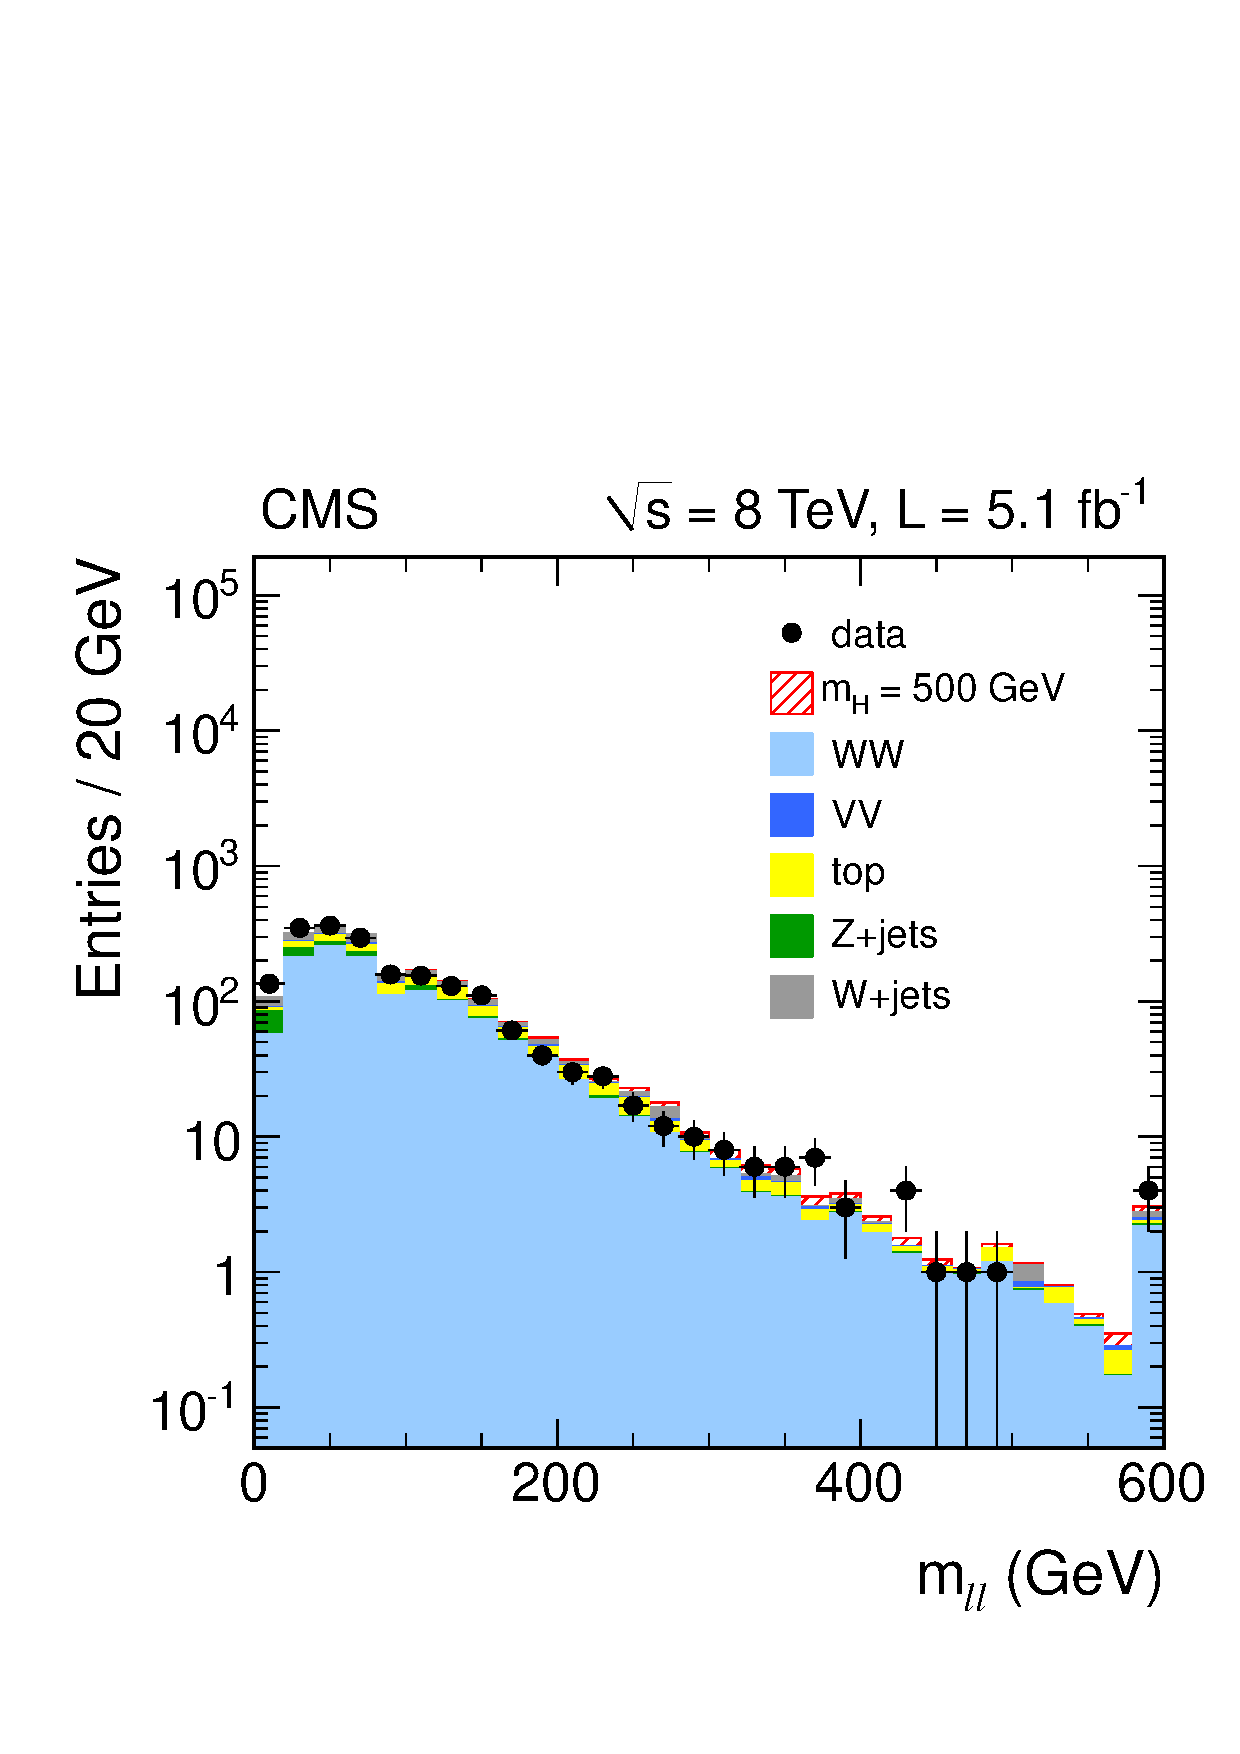
\includegraphics[width=0.49\textwidth]{plots/hww2l2n_highmass_mll500_0j.pdf}
%   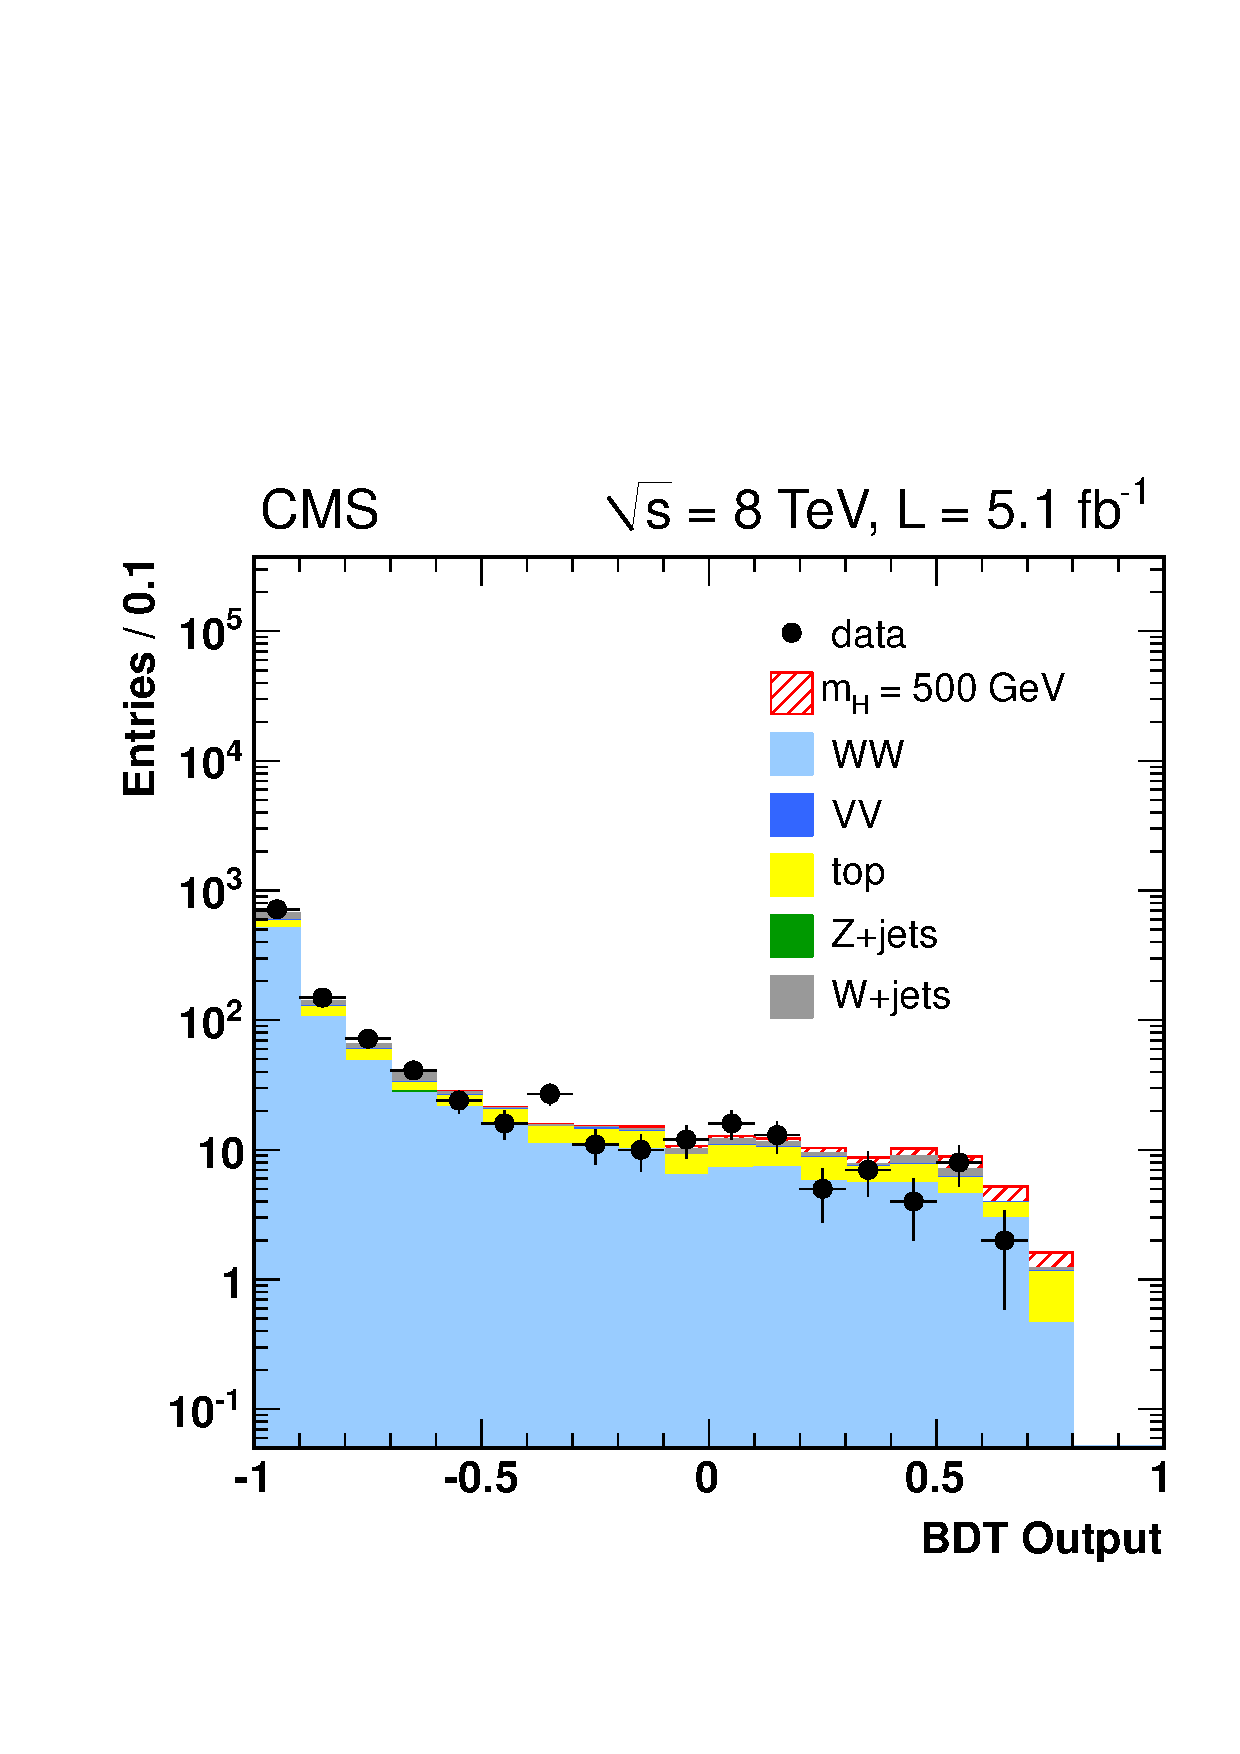
\includegraphics[width=0.49\textwidth]{plots/hww2l2n_highmass_bdt500_0j.pdf}
   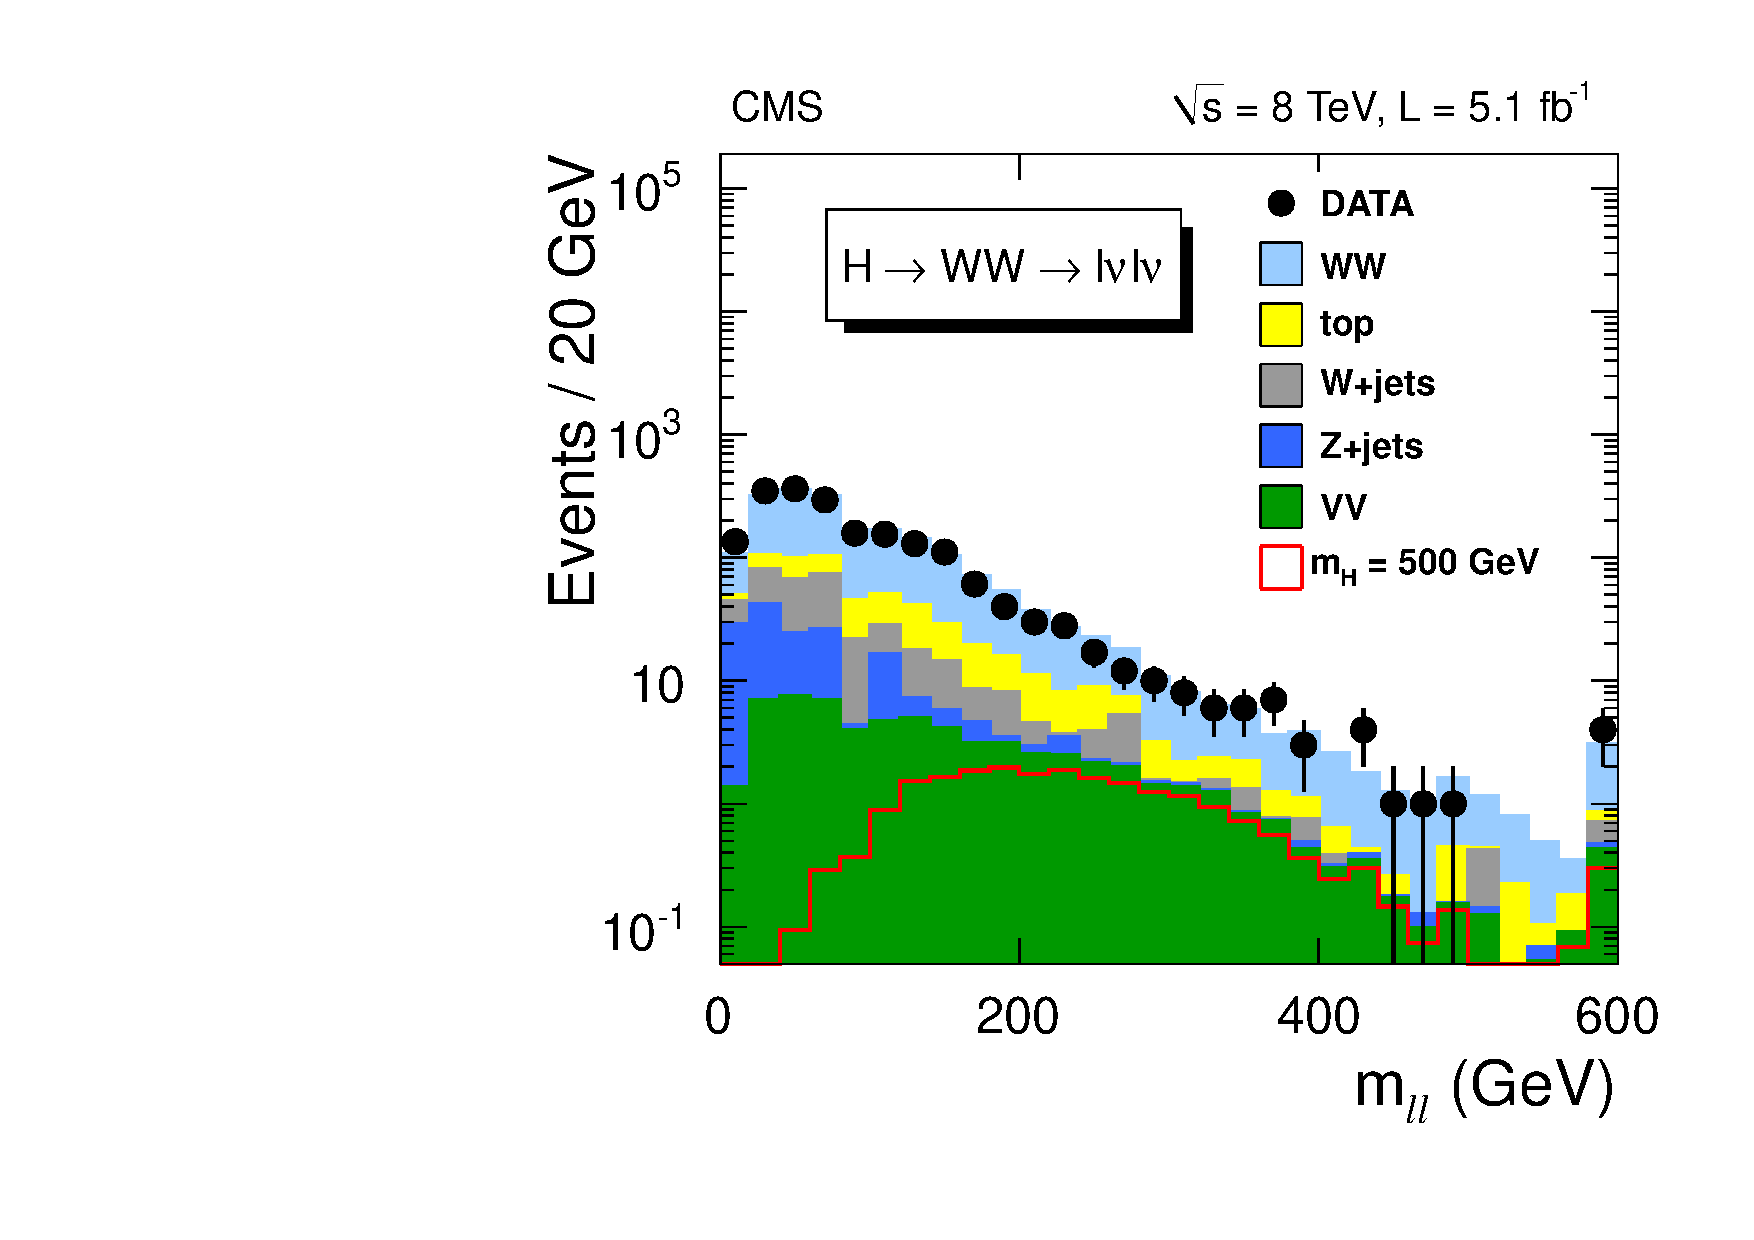
\includegraphics[width=0.49\textwidth]{figures/WW2l2nuMass.pdf}
   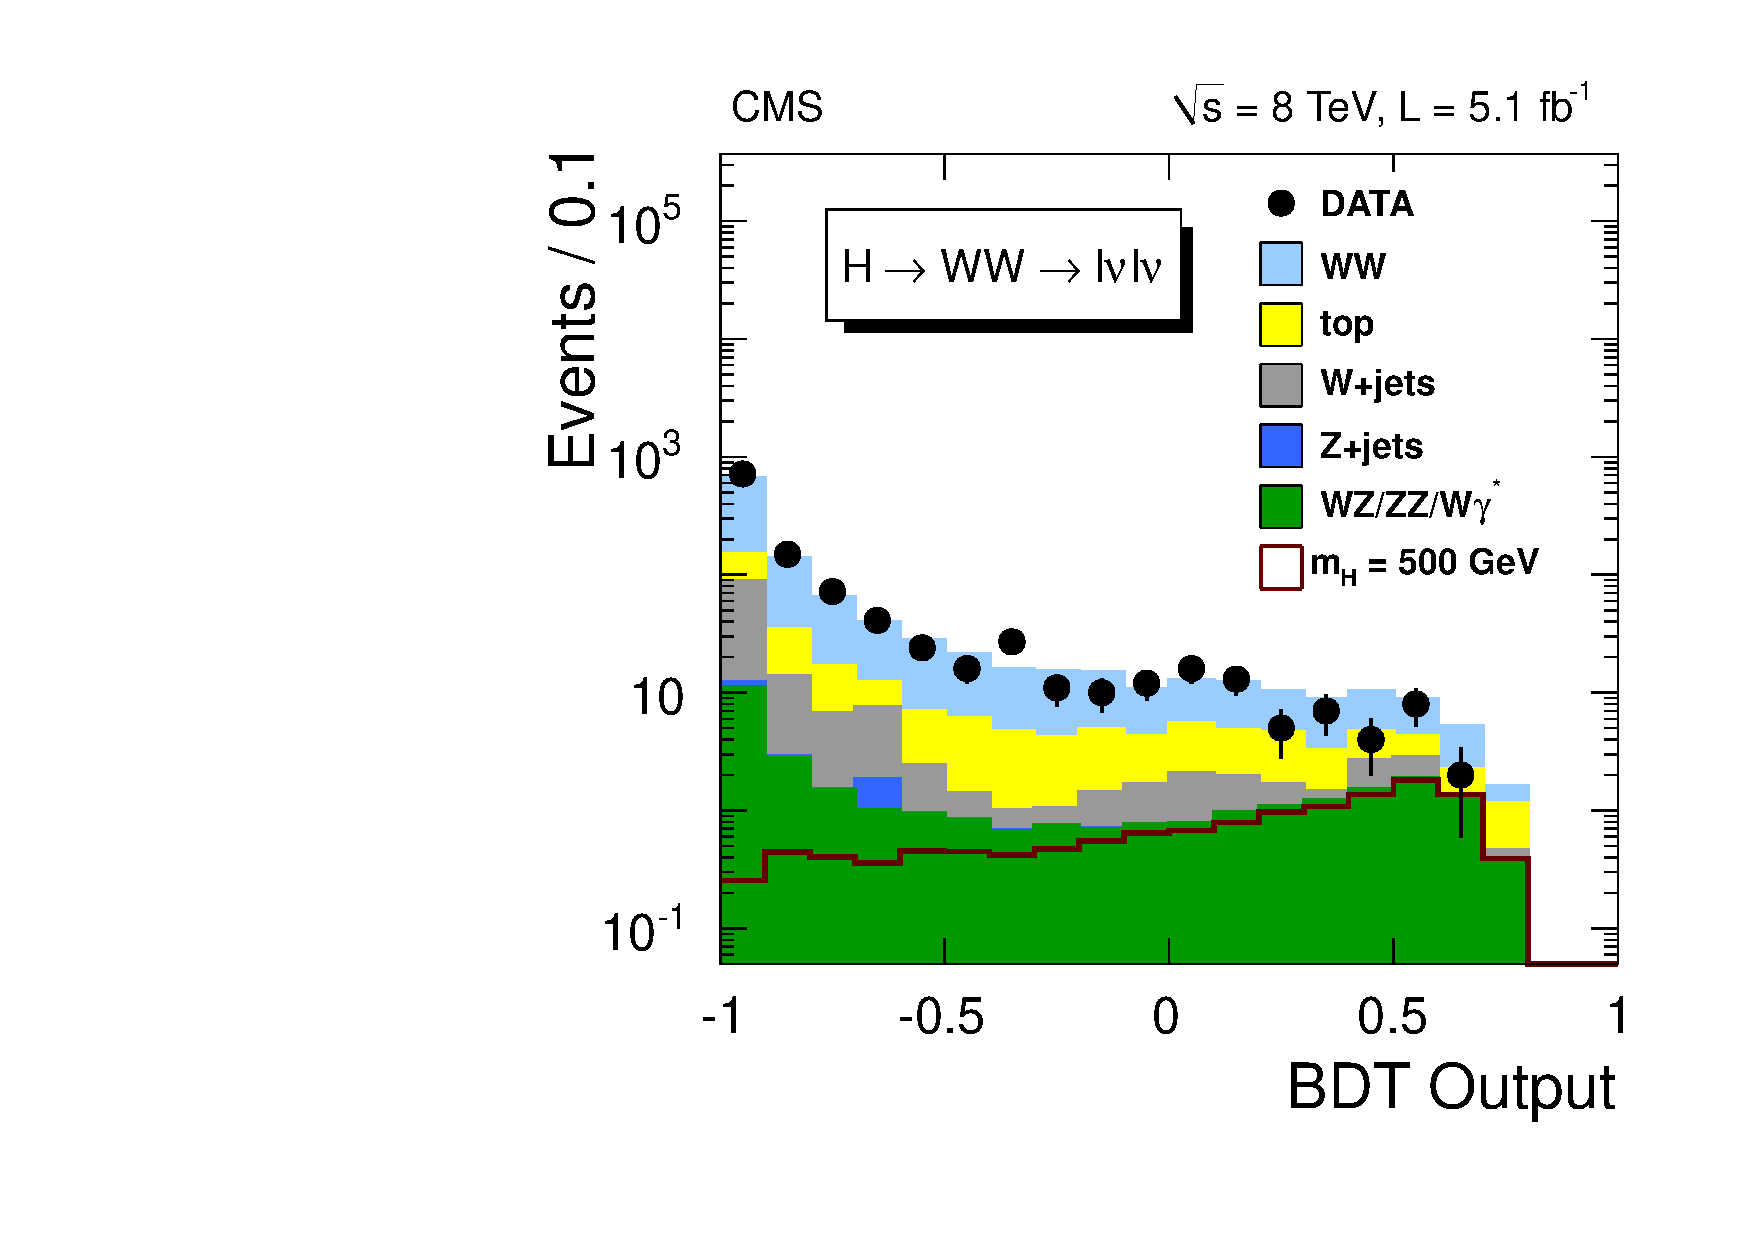
\includegraphics[width=0.49\textwidth]{figures/WW2l2nuBDT.pdf}
   \caption{ $\PW\PW \to \ell\nu\ell\nu$ channel. (a) Distributions of the dilepton mass between the
   two selected leptons in the 0-jet category, for data (points with
   error bars), for the main backgrounds (stacked histograms), and for
   a SM Higgs boson signal with $\mH= 500\GeV$ (superimposed
   histogram). The standard pre-selection is applied.  (b) BDT-classifier
   distributions for signal and background events for a SM
   Higgs boson with $\mH=500\GeV$ and for the main backgrounds at the
   BDT selection level in the 0-jet bin different-flavor final state.}
\label{fig:hww2l2n_bdt_500}
\end{figure}

The backgrounds that remain after applying the final selection criteria are estimated by a combination of techniques~\cite{CMSobservation125}. The $\ttbar$ background is estimated by extrapolation from the observed 
number of events with the b-tagging cut inverted. The Drell--Yan background measurement is based on extrapolation
from the observed number of $\Pe^+\Pe^-$, $\Pgm^+ \Pgm^-$ events with the $\cPZ$-veto cut inverted. The background 
of $\PW$+jets and QCD multi-jet events is estimated by measuring the number of events with one lepton passing a loose
cut on isolation. The probability for such loosely-isolated fake leptons to pass the tight isolation cut is measured in
data using multi-jets events. The non-resonant $\WW$ contribution is estimated from simulation.

Experimental effects, theoretical predictions, and the choice of event generators are considered as sources of
uncertainty, and their impact on the signal efficiency is assessed. The impact on the kinematic distributions is also considered for the BDT analysis. The overall signal efficiency uncertainty is estimated to be about 20\%, and is
dominated by the theoretical uncertainty associated with missing QCD higher-order corrections and PDF uncertainties. The total uncertainty on the background estimation in the $\Hww$ signal region is about 15\%, dominated by the
statistical uncertainty on the observed number of events in the background control regions.

After applying the final selections, no evidence of a SM Higgs boson is observed over the mass range considered in this paper. Upper limits are derived on the ratio of the product of the Higgs boson production cross section and the $\Hi \to \WW$ branching fraction, $\sigma_{\Hi} \times \mathrm{BR}(\Hi \to \WW)$, to the SM expectation. The observed and expected upper limits with all categories combined are shown in Figure~\ref{fig:hwwlvlvlim}. At least part of the excess observed at
low masses may be ascribed to the presence of the new boson at mass about 125 GeV that is not accounted for in the analysis.

\begin{figure}[htbp]
  \centering
%  \subfigure[]{
%  \includegraphics[width=0.48\textwidth]{plots/hwwlvlvlimit8tev.pdf}
%  }  
%   \subfigure[]{ 
  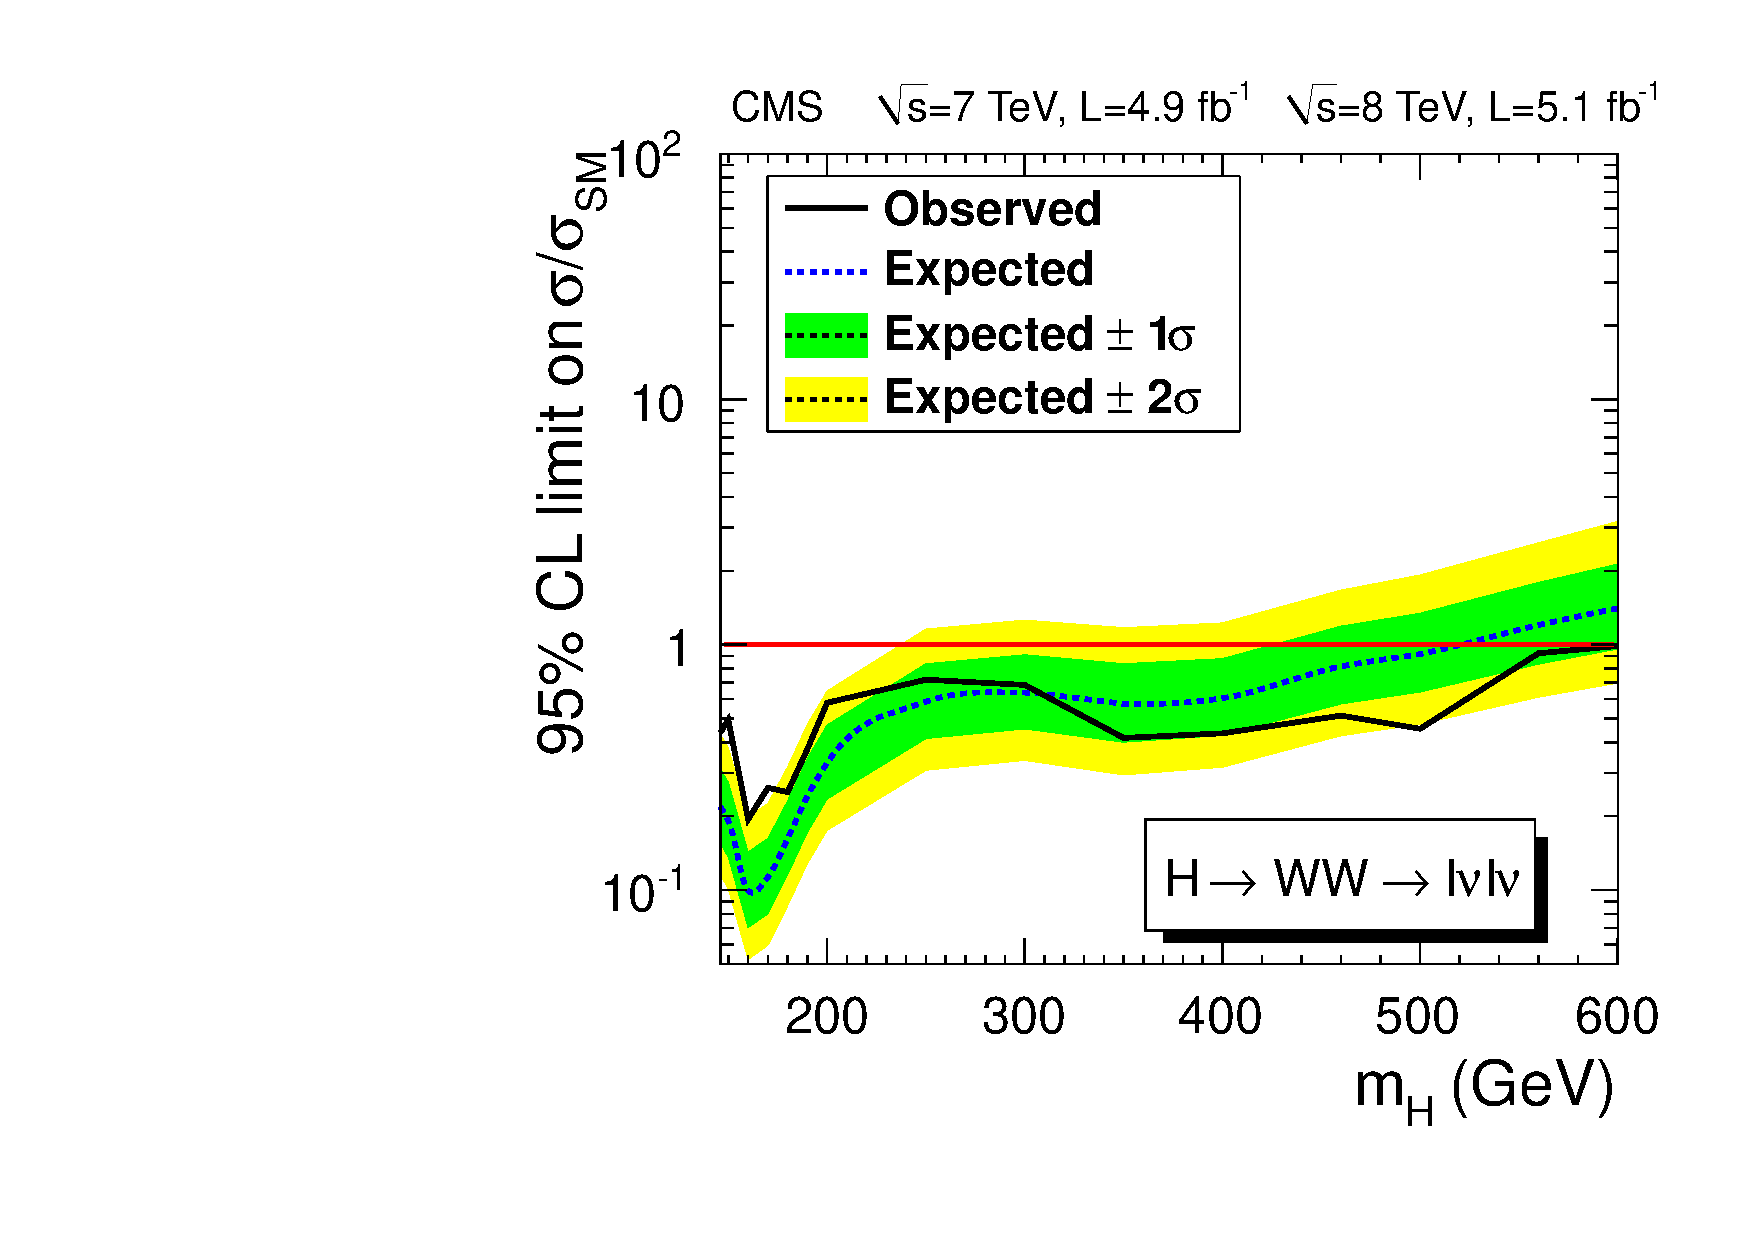
\includegraphics[width=0.6\textwidth]{figures/WW2l2nuLimit.pdf}
%  }   
  \caption{\label{fig:hwwlvlvlim}Observed (solid) and expected
    (dashed) 95\% CL upper limit on the ratio of the product of production cross
    section and branching ratio to the SM expectation for the Higgs boson obtained using
    the asymptotic CL${}_{\textrm{S}}$ technique in the $\PW\PW \to \ell\nu\ell\nu$ channel. The 68\% and 95\%
    ranges of expectation for the background-only model are also shown
    with green and yellow bands, respectively. The solid line at 1
    indicates the SM expectation.} 
%The limit combines data from both
%    7 TeV and 8 TeV collisions.},
\end{figure}

\subsection{$\PH \to \PW\PW \to \ell\nu \rm{qq}$}

The $\WW$ semileptonic channel has the largest branching fraction of all the channels presented in this paper.
Its advantage over the fully leptonic final state is that it has a reconstructable Higgs boson mass peak~\cite{intro2}. This
comes at the price of a large \PW+jets background. The level to which this background can be controlled
largely determines the sensitivity of the analysis. 

The reconstructed electrons (muons) are required to have 
$\PT>35(25)\GeV$, and are restricted to $|\eta|<2.5(2.1)$.
The jets are required to have 
$\PT>30\GeV$ and $|\eta|<2.4$, and to not
overlap with the leptons, 
with the overlap determined by a cone around the lepton axis of radius $\Delta R = 0.3$. 
%The analysis is performed in four categories. Events with electrons and muons,
%and also with two or three jets located within the tracker acceptance ($|\eta| < 2.4$) and with
%$\PT>30\GeV$ are analysed separately.
%Jets that overlap isolated leptons are not considered, with the overlap
%determined by a cone around the lepton axis of radius $\Delta R = 0.3$. Since initial and final
%state gluon radiation can result in an extra jet, only events with exactly two or three jets
%are selected for the analysis.
Events with the electrons and muons, and with exactly two or three jets are analysed separately,
giving four categories in total.
%Events with electrons and muons are analysed separately. Since initial and final state gluon radiation can result in an additional jet, events with two or three jets above are selected for the analysis, and also analysed separaetly,
%giving four analysis categories in total. Jets are required to have $|\eta|<2.4$ and $\PT>30\GeV$, and jets that overlap isolated leptons are not considered, with the overlap determined by a cone around the lepton axis of radius $\Delta R = 0.3$. 
%% ED: Do we really mean *isolated* lepton here? 
The combination of the two highest-$\PT$ jets is assumed as the hadronic $\PW$ candidate. According to simulation, in the case of 2(3)-jet events, the correct jet-combination rate varies from 68(26)\% for $\mH = 200\GeV$ to 88(84)\% for
$\mH = 600\GeV$. Events with an incorrect dijet combination result in a broad non-peaking background in the $m_{\WW}$ spectrum.

The leptonic $\PW$ candidate is reconstructed from the $(\ell,\MET)$ system. Events are required to have $\MET>\text{30(25)}\GeV$ for the electron(muon) categories. To reduce the background from processes that do not
contain $\PW\to\ell\nu$ decays, requirements of $m_{\rm{T}}^{\ell,\MET}>30\GeV$ and
$|\Delta\phi_{\textrm{leading jet,\MET}}| >$ 0.8 (0.4) are imposed for electrons (muons). These criteria reduce the QCD multi-jet background, for which in many cases the $\MET$ is generated by the overestimate of the energy of a jet.

To improve the $m_{\WW}$ resolution, both $\PW$ candidates are constrained in a kinematic fit to the $\PW$-boson
mass to within its known width, with the longitudinal component of the neutrino momentum, $|p_{\textnormal{z}}|$ unknown. The ambiguity in the second-order kinematic equation is resolved by taking the solution that yields the smaller $|p_{\textnormal{z}}|$ value for the neutrino.  

%% ED: What does 'constrained to the W mass to within its known width' mean? Is it just constrained to the W mass, or allowed to float within some range?

To exploit the differences in kinematics between signal and background events, a likelihood discriminant is constructed
that incorporates a set of variables that best distinguishes the Higgs signal from the \PW+jets background. 
These variables comprise five angles between the Higgs decay products, that fully describe the Higgs production kinematics~\cite{Gao:2010qx}; the $\PT$ and rapidity of the $\WW$ system; and the lepton charge.
The likelihood discriminant is optimized with dedicated simulation samples for several discrete Higgs boson mass hypotheses,
for each lepton flavor ($\Pe$, $\Pgm$) and for each jet multiplicity (2-jet, 3-jet) independently. Four different optimizations are therefore obtained per mass hypothesis. For each of them, events are retained if they
survive a simple selection on the likelihood discriminant, chosen in order to optimise the expected limit for the Higgs cross-section.

%% ED: Please check that I have reworded the last sentence correctly, and preserved the meaning.

To extract simultaneously the relative normalizations of all background components in the signal region, an
unbinned maximum likelihood fit is performed on the invariant mass distribution of the dijet system, $m_{jj}$.
The fit is performed independently for each Higgs boson mass hypothesis. The signal region corresponding to the $\PW$
mass window, $65\GeV < m_{jj} < 95\GeV$, is excluded from the fit. The shape of the $m_{jj}$ distribution for the
$\PW$+jets background is taken from simulation for Higgs boson mass hypotheses at or below $200\GeV$. For higher masses,
insufficient numbers of simulated events are available, and the shape is therefore described analytically using an exponential function. The overall normalization of the \PW+jets component is allowed to vary in the fit. The shapes for
other backgrounds (electroweak diboson, \ttbar, single top, and Drell--Yan plus jets) are based on simulation, and their
normalizations are constrained to theoretical predictions, within the corresponding uncertainties.
The multijet background normalization is estimated from data by relaxing lepton isolation and identification requirements.
Its contribution to the total number of events is evaluated from a separate two-component likelihood fit to the $m_{\rm{T}}^{\ell,\MET}$ distribution, and constrained in the $m_{jj}$ fit according to this fraction within
uncertainties. For electrons, the multijet fraction accounts for several percent of the event sample, depending on the
number of jets in the event, while for muons it is negligible.


Limits are established based on the measured invariant mass of the $\WW$ system, $m_{\ell\nu jj}$. The
binned shapes of
$m_{\ell\nu jj}$ for total background, signal and data for each mass hypothesis and event category are
constructed as
input to the limit-setting procedure. The $m_{\ell\nu jj}$ shape for the major background, \PW+jets,
is extracted from data as a linear combination of the shapes measured in two signal-free sideband
regions of $m_{jj}$ ($55\GeV <m_{jj} < 65\GeV$,
$95\GeV < m_{jj} < 115\GeV$). The relative fraction of the two sidebands is motivated through
simulation, separately for
each Higgs boson mass hypothesis, by minimizing the $\chi^2$ between the interpolated shape in the
signal region and the expected one. The $m_{\ell\nu jj}$ shape for multijet background events is
obtained from data with the procedure described above.
All other background categories use the $m_{\ell\nu{}jj}$ shape
from simulation.

The $m_{jj}$ and $m_{\ell\nu jj}$ distributions with final background estimates are 
shown in Figure~\ref{fig:lvjjfits}, with
selections optimized
for a $500\GeV$ Higgs boson mass hypothesis, for the $(\Pgm,2\rm{jets})$ category. 
The final background $m_{\ell\nu{}jj}$ distribution is obtained by summing
up all the individual contributions.
To avoid statistical fluctuations due to the low event count,
the distribution is fit with an exponential function. This function
is then used for the
limit evaluation. All uncertainties arising from interpolation and fit procedures are propagated to
the limit calculation as
systematic uncertainties.


%Limits are established based on the measured invariant mass of the $\WW$ system, $m_{\ell\nu jj}$. The binned shapes of
%$m_{\ell\nu jj}$ for total background, signal and data for each mass hypothesis and event category are constructed as
%input to the limit-setting procedure. The $m_{\ell\nu jj}$ shape for the major background, \PW+jets, is extracted from data as a linear combination of the shapes measured in two signal-free sideband regions of $m_{jj}$ ($95\GeV <m_{jj} < 115\GeV$,
%$55\GeV < m_{jj} < 65\GeV$). The relative fraction of the two sidebands is motivated through simulation, separately for
%each Higgs boson mass hypothesis, by minimizing the $\chi^2$ between the interpolated shape in the signal region and the expected one. The $m_{\ell\nu jj}$ shape for multijet background events is obtained from the data sample selected for the $m_{jj}$ fit and normalized according to the fit results. All other background categories use the $m_{\ell\nu{}jj}$ shape
%from simulation.

%% DN: 'extrapolated' -> 'interpolated' I think?

%Examples of the $m_{jj}$ and $m_{\ell\nu jj}$ fits are shown in Figure~\ref{fig:lvjjfits}, with selections optimized
%for a $500\GeV$ Higgs boson mass hypothesis, for the $(\Pgm,2\rm{jets})$ category. The distributions of the interpolated 
%\PW+jets background in the signal region are also shown. Because of the low event count, the shapes are regularized by
%means of an exponential fit. The uncertainties from both fits are propagated to the limit calculation as 
%systematic uncertainties.

\begin{figure}[htbp]
  \centering
  \subfigure[]{
%  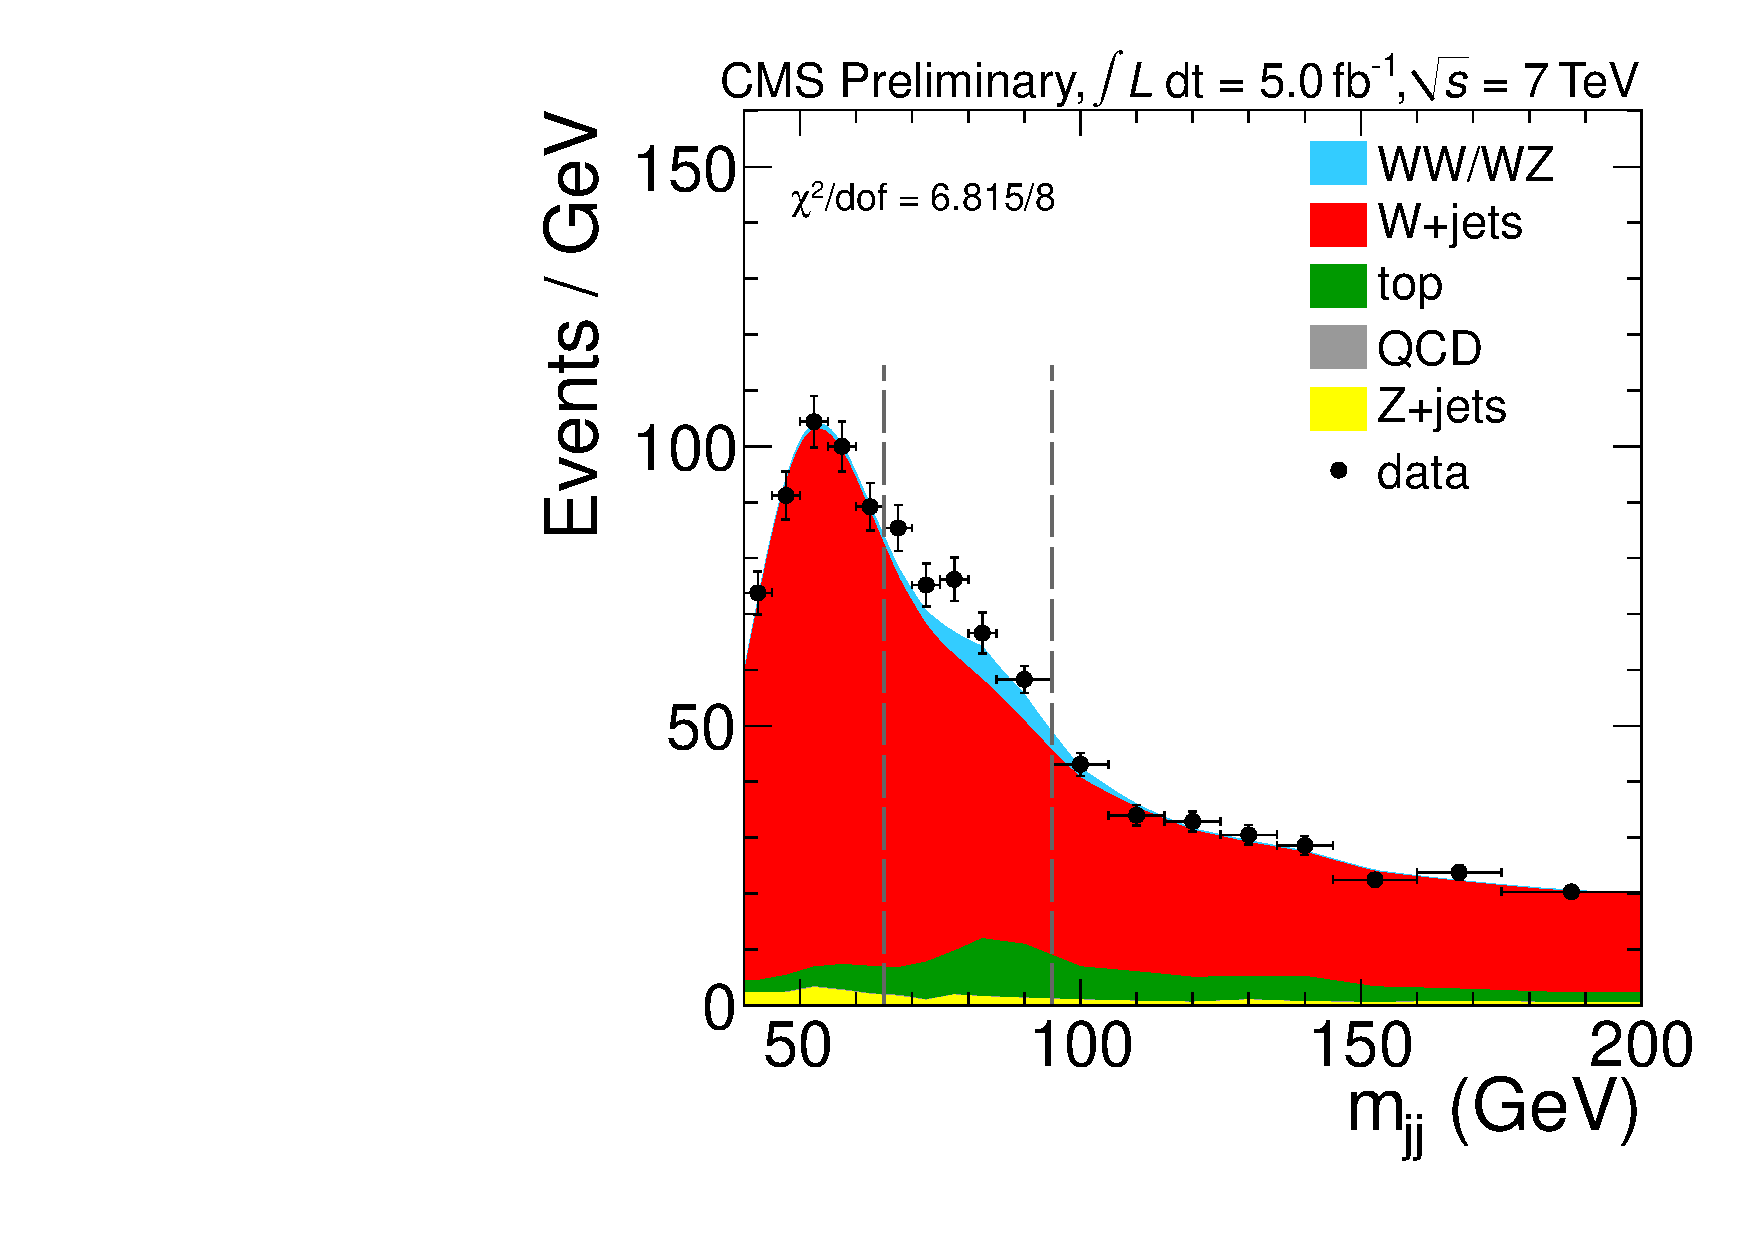
\includegraphics[width=0.48\textwidth]{plots/H500_Mjj_Muon_2jets_Stacked.pdf}
  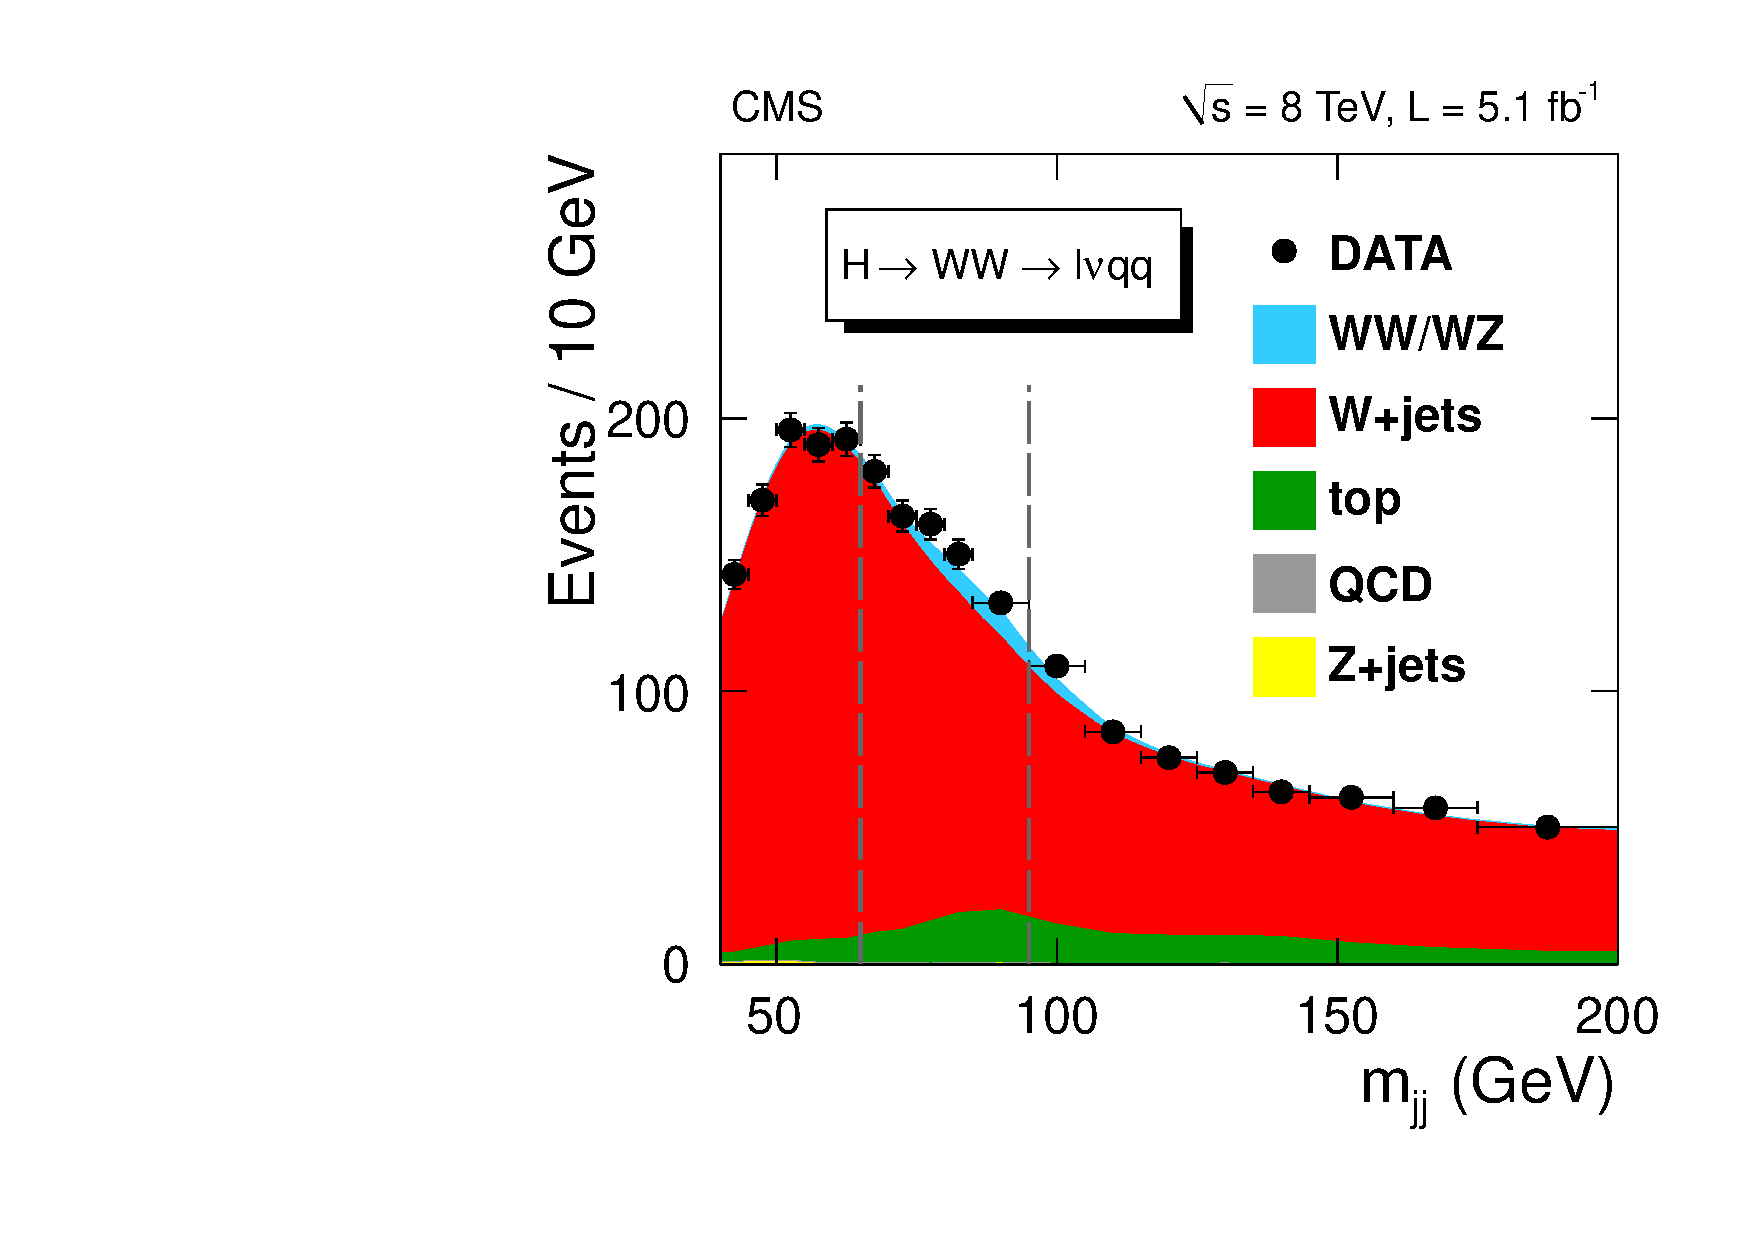
\includegraphics[width=0.48\textwidth]{figures/WW2l2qMjj.pdf}
  }  
   \subfigure[]{ 
%  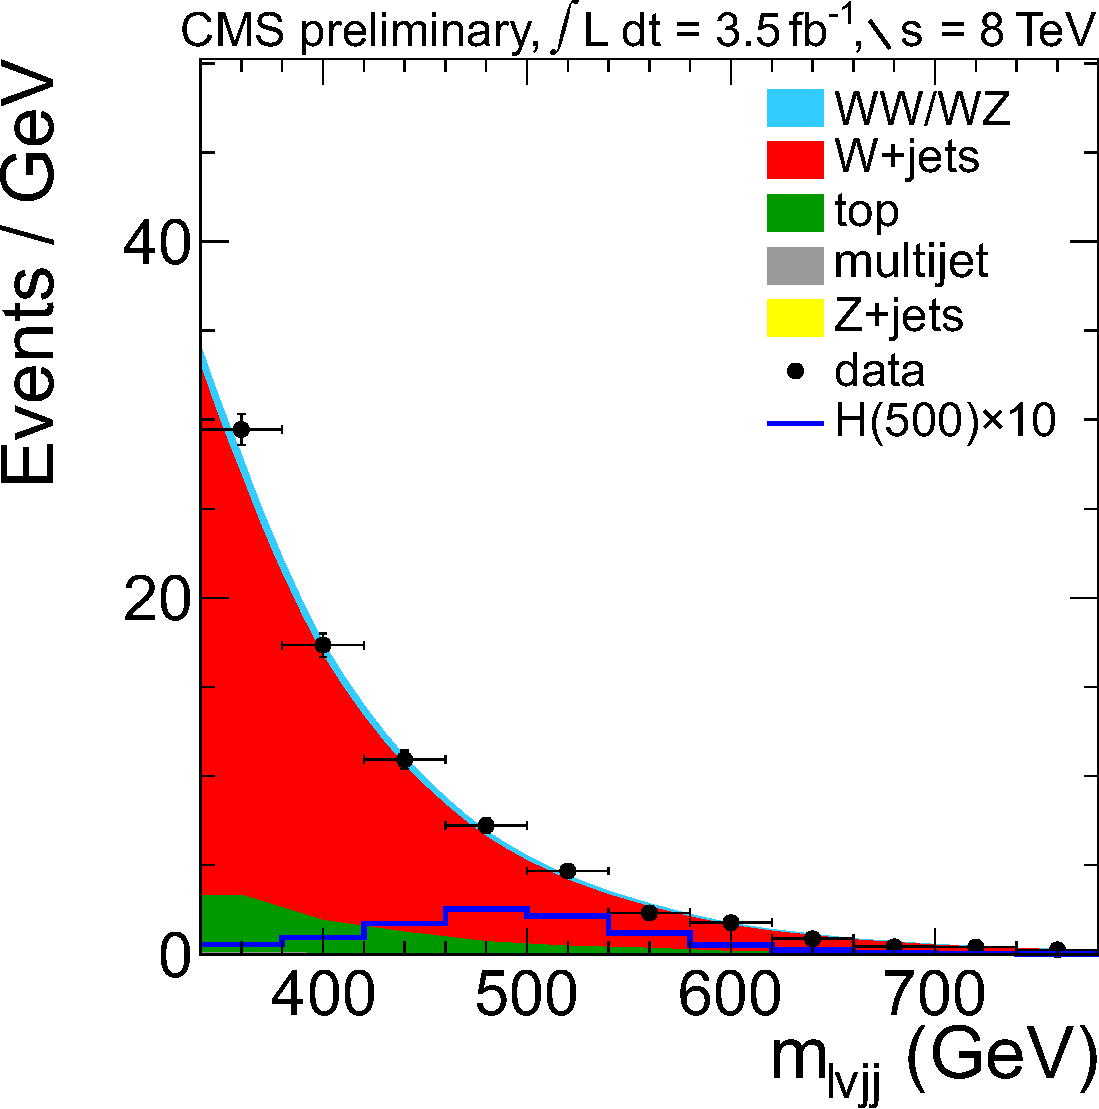
\includegraphics[width=0.48\textwidth]{plots/H500_Mlvjj_Muon_2jets_Stacked.pdf}
  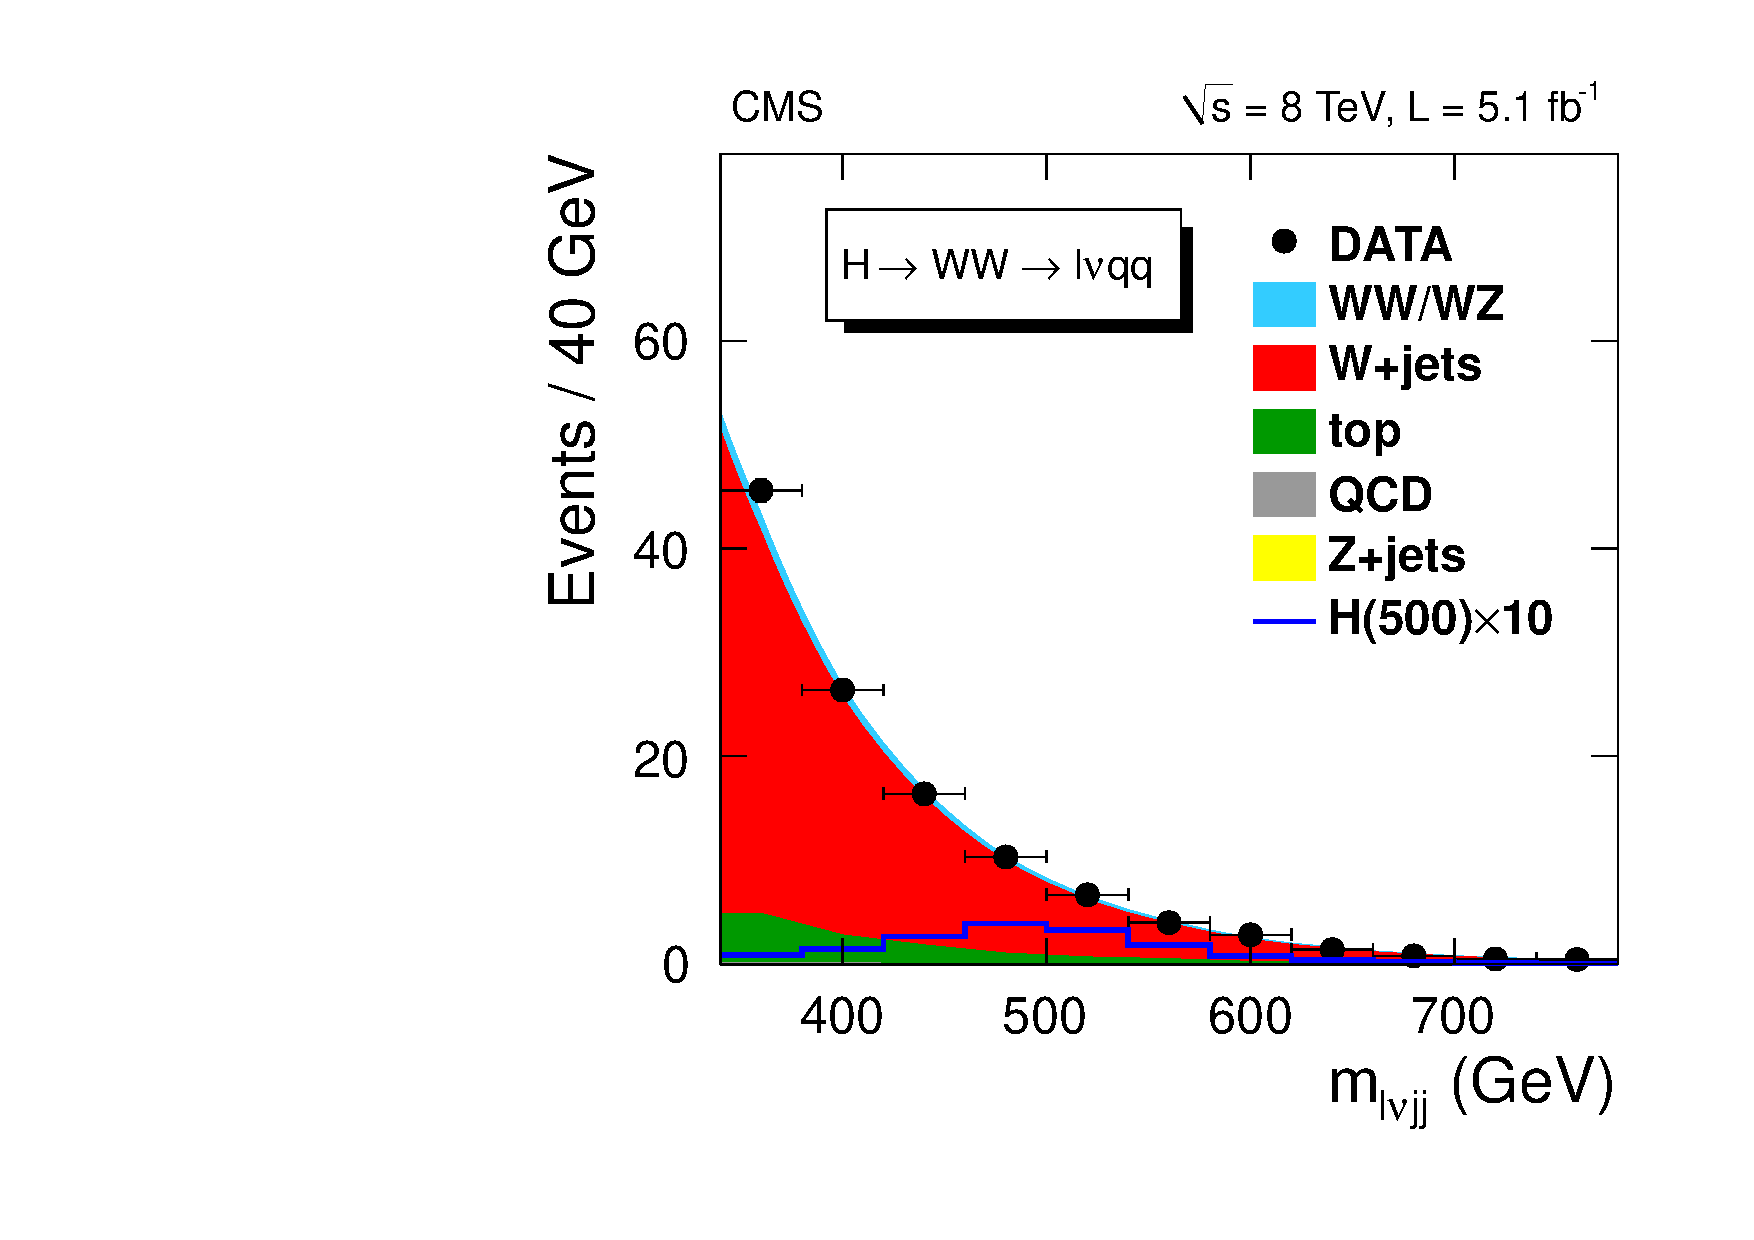
\includegraphics[width=0.48\textwidth]{figures/WW2l2qMass.pdf}
  }   
%  \subfigure[]{ 
%  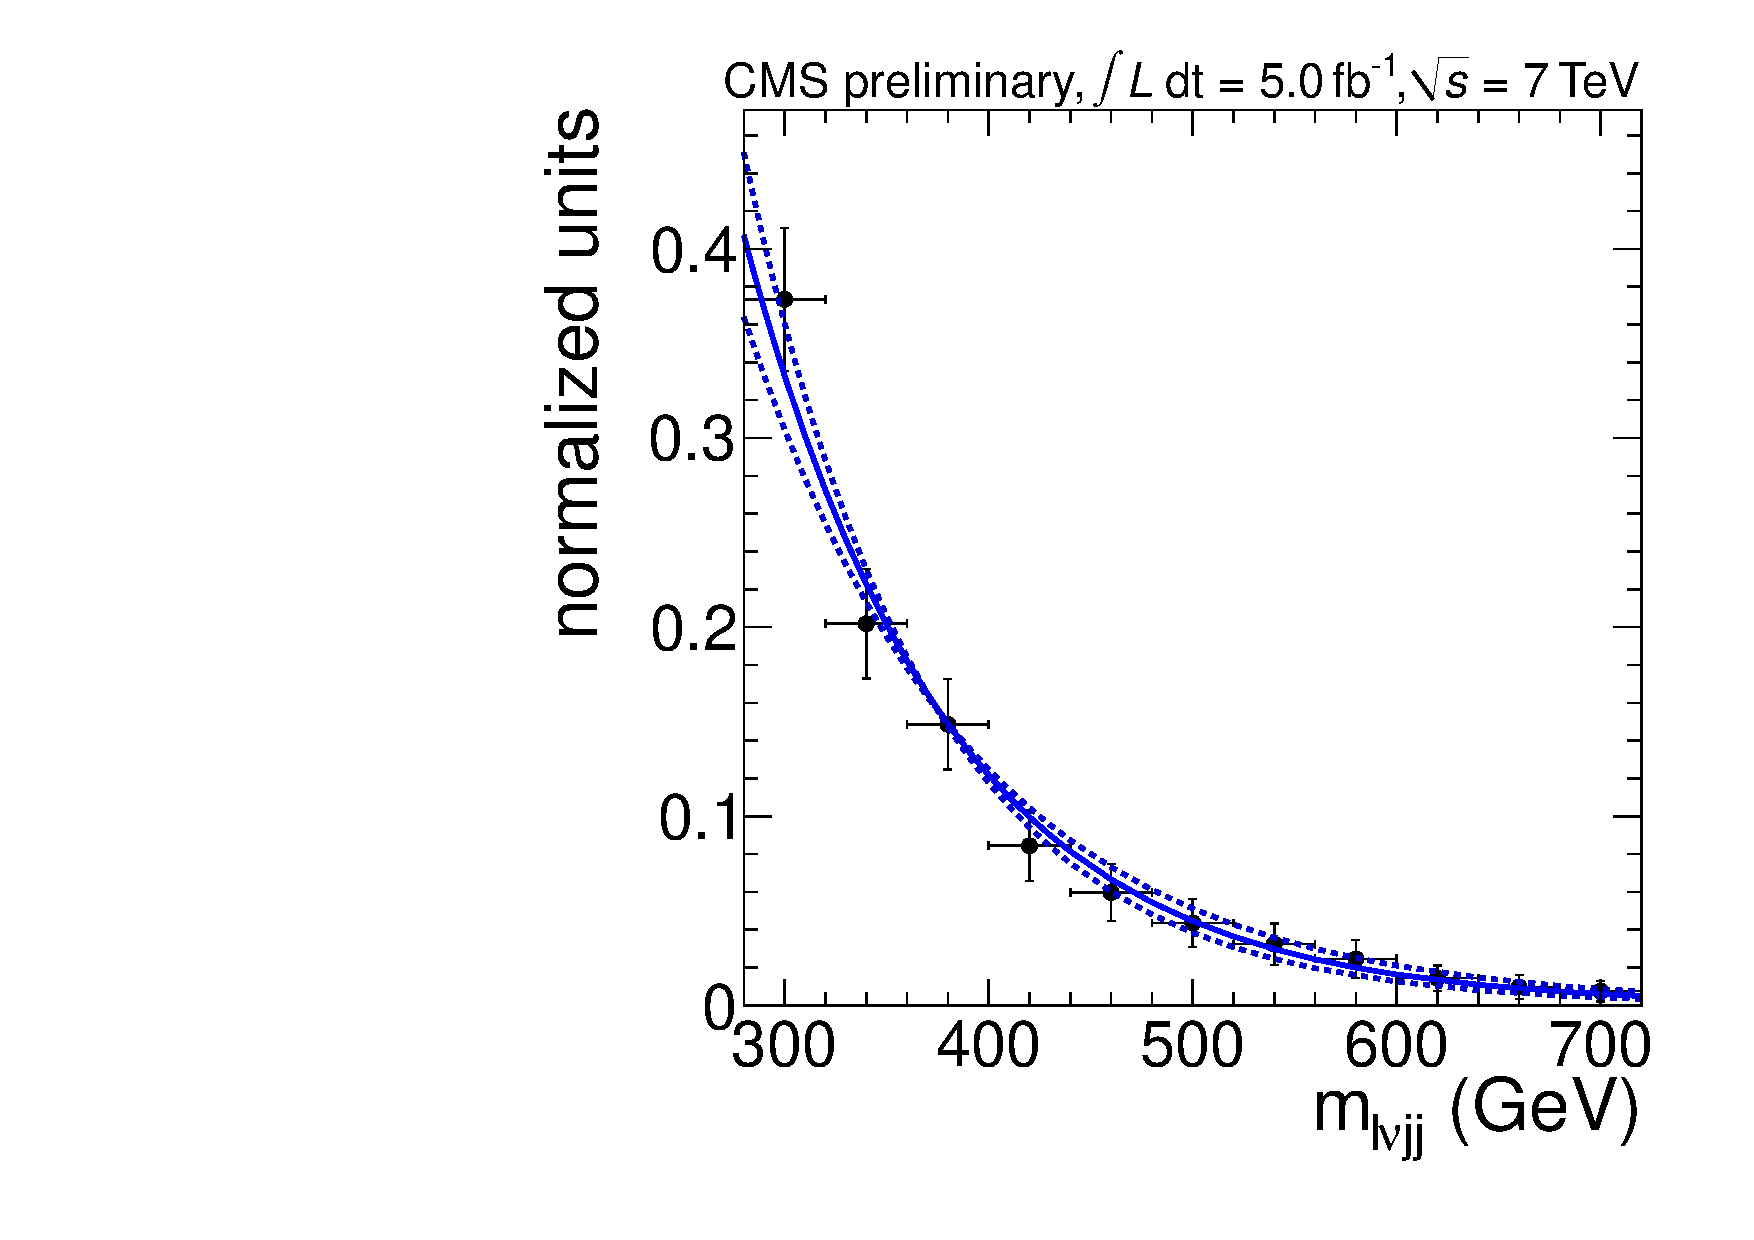
\includegraphics[width=0.32\textwidth]{plots/H500_Mlvjj_Muon_2jets_WpJShape.pdf}
%  }  
%  \caption{\label{fig:lvjjfits} Fit plots for the mass hypothesis
%    $\mH=500\GeV$, muon 2-jet category in the $\PH \to \PW\PW \to \ell\nu \rm{qq}$ channel.  (a) The dijet invariant mass
%    distribution with the fit projections of the background components.
%    The vertical lines corresponds to the signal region of this analysis
%    $65\GeV < m_{jj}
%    < 95\GeV$.  %(c) The distribution of the extrapolated background
%    (b) The $\WW$ invariant mass distribution with the fit projections of
%    the background components in the signal region.
%    The black symbols represent the data.}
%    interpolated points, while the blue curve is the smooth
%    parametrization using an exponential function.}  
%    The dashed bands
%    show the envelope of the systematic uncertainty in the shape
%    extrapolation. }
  \caption{\label{fig:lvjjfits} Invariant mass distributions for the
    $\mH=500\GeV$ mass hypothesis, $(\Pgm,2\rm{jets})$ category in the
    $\PH \to \PW\PW \to \ell\nu \rm{qq}$ channel.
    (a) The dijet invariant mass
    distribution with the major background contributions.
    The vertical lines corresponds to the signal region of this analysis
    $65\GeV < m_{jj}
    < 95\GeV$.
    (b) The $\WW$ invariant mass distribution with the major background
    contributions in the signal region.
    }
\end{figure}

The largest source of systematic uncertainty is due to $m_{\ell\nu jj}$-shape uncertainty of the \PW+jets background.
The only other uncertainty assigned to background is the normalization uncertainty from the $m_{jj}$ fit. Both of these 
uncertainties are estimated from data. All other systematic uncertainties are applied to signal processes. The dominant 
signal uncertainties include theoretical uncertainties for the cross section (14-19\% for gluon fusion)~\cite{LHCHiggsCrossSectionWorkingGroup:2011ti} and exclusive jet binning effects on scale (4-28\%), as well as the 
efficiency of the likelihood selection (10\%). The latter effect is computed by taking the relative difference in efficiency 
between data and simulation using a control sample of top pair events in data. These events are good proxies for the signal,
since in both cases the primary production mechanism is gluon-gluon fusion, and the semi-leptonic final states contain
decays of two W bosons.

The upper limits on the ratio of the production cross section for the Higgs boson compared to the SM expectation are 
presented in Figure~\ref{fig:hwwlvjjlim}. 

\begin{figure}[htbp]
  \centering
%   \subfigure[]{
%  \includegraphics[width=0.48\textwidth]{plots/hwwlvjjlimit8tev.pdf}
%   }
%  \subfigure[]{
  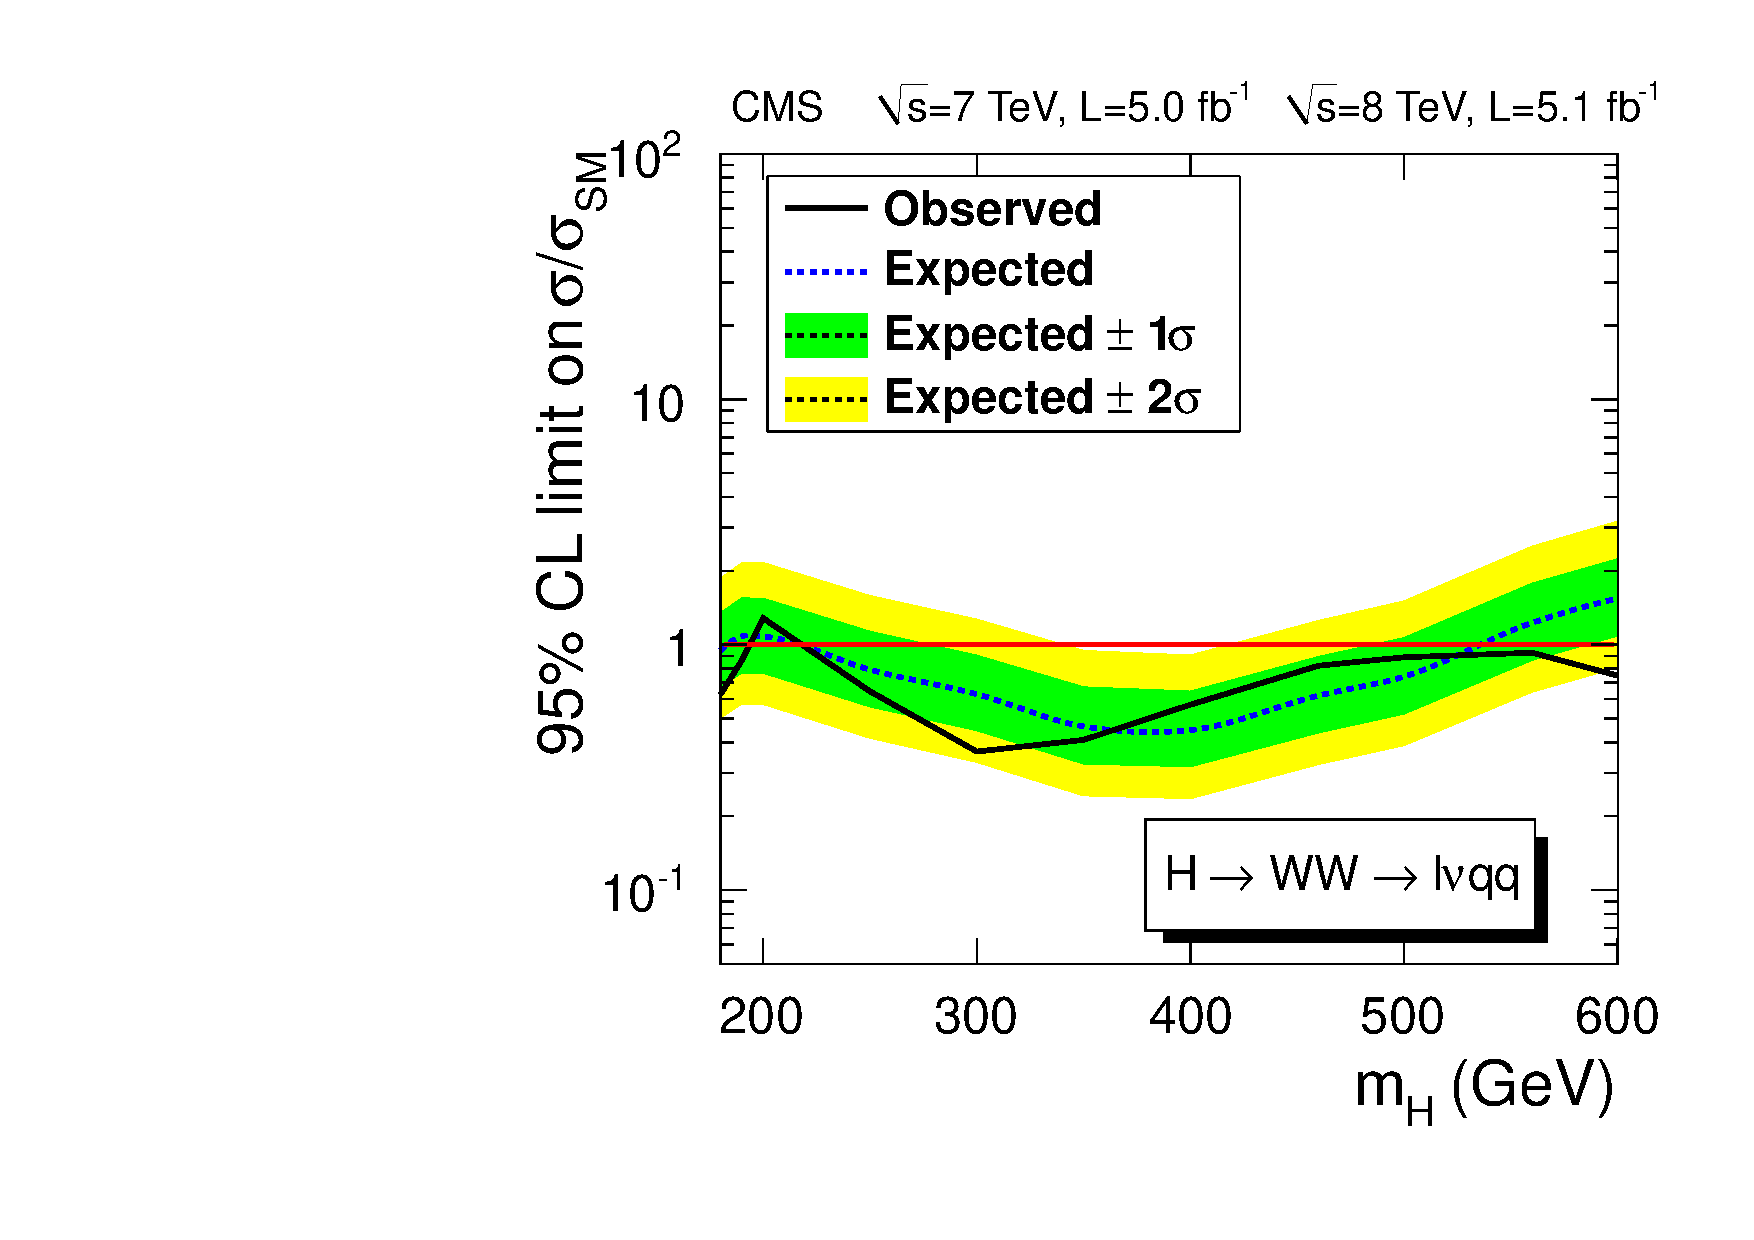
\includegraphics[width=0.6\textwidth]{figures/WW2l2qLimit.pdf}
%  }
  \caption{\label{fig:hwwlvjjlim} Observed (solid) and expected
  (dashed) 95\% CL upper limit on the ratio of the product of production cross
  section and branching ratio to the SM expectation for the Higgs boson in the WW
  semileptonic channel.}  
%The limit combines data from both 7 TeV and 8
%  TeV collisions.}
\end{figure}

%%%%%%
\def\PZ{\ensuremath{\mathrm{Z}}\xspace}
\def\PV{\ensuremath{\mathrm{V}}\xspace}
\def\ZZ{\ensuremath{\PZ\PZ}\xspace}
\def\WW{\ensuremath{\PW\PW}\xspace}
\def\WZ{\ensuremath{\PW\PZ}\xspace}
\def\QT{\ensuremath{q_{\mathrm{T}}}\xspace}
\def\PT{\ensuremath{p_{\mathrm{T}}}\xspace}
\def\VECPT{\ensuremath{\vec{p}_{\mathrm{T}}}\xspace}
\def\VECQT{\ensuremath{\vec{q}_{\mathrm{T}}}\xspace}
\def\ET{\ensuremath{E_{\mathrm{T}}}\xspace}
\def\MET{\ensuremath{{E\!\!\!/}_{\mathrm{T}}}}
\def\PFMET{\ensuremath{\MET}}
\def\PUMET{\ensuremath{{\MET}^{\mathrm{PU}}}}
\def\PUMETMIN{\ensuremath{{\MET}^{\mathrm{PU,min}}}}
\def\CORRMET{\ensuremath{{\MET}^{\mathrm{corr}}}}

\def\SIGBRZZee{\ensuremath{ [\,\sigma\times {\cal{B}}\,](\ \, \pp\to \ZZ \to \Pe\Pe\nu\nu\ ) }\xspace } 
\def\SIGBRZZmm{\ensuremath{ [\,\sigma\times {\cal{B}}\,](\, \pp\to \ZZ \to \Pgm\Pgm\nu\nu\ ) }\xspace } 
\def\SIGBRZZll{\ensuremath{ [\,\sigma\times {\cal{B}}\,](\ \, \pp\to \ZZ \to \ell\ell\nu\nu\ ) }\xspace } 
\def\SIGZZ{\ensuremath{ \sigma( \pp\to\ZZ )  }\xspace}

\def\NbkgEleWjets{ \ensuremath{ 3.4 \pm 1.1 \pm 1.5 }\xspace } 
\def\NbkgEleWGam{ \ensuremath{ 1.5 \pm 0.4  }\xspace } 
\def\NbkgEleTop{   \ensuremath{ 0.7 \pm 0.4 }\xspace } 
\def\NbkgEleNonPeaking{ \ensuremath{ 5.6 \pm 2.1 }\xspace } 
\def\NbkgElePeakingZJ{ \ensuremath{ 3.6 \pm 0.9 }\xspace } 
\def\NbkgElePeakingZG{ \ensuremath{ 0.3 \pm 0.2 }\xspace } 

\def\NElePeaking{ \ensuremath{ 11.2 \pm 5.2\,{\mathrm{(stat)}} \pm 1.6\,{\mathrm{(bkg)}} }\xspace }
\def\NElePeakingWithWZ{ \ensuremath{ 14.4 \pm 5.2\,_{\mathrm{(stat)}} \pm 1.1\,_{\mathrm{(bkg)}} }\xspace }
\def\NEleNonPeaking{ \ensuremath{ 14.1 \pm 5.2\,_{\mathrm{(stat)}} \pm 1.6\,_{\mathrm{(bkg)}} }\xspace }

\def\NbkgMuoWjets{ \ensuremath{ 0.0\,^{+0.9}_{-0.0} }\xspace }
\def\NbkgMuoTop{   \ensuremath{ 1.0 \pm 0.5 }\xspace } 
\def\NbkgMuoNonPeaking{ \ensuremath{ 1.0\,^{ \pm 1.4 }_{-0.5} }\xspace } 
\def\NbkgMuoPeakingZJ{ \ensuremath{ 1.6 \pm 0.4 }\xspace } 
\def\NbkgMuoPeakingZG{ \ensuremath{ 0.1 \pm 0.1 }\xspace } 

\def\NMuoPeaking{ \ensuremath{ 10.4 \pm 4.8\,{\mathrm{(stat)}}\pm 1.1\,{\mathrm{(bkg)}}  }\xspace }
\def\NMuoPeakingWithWZ{ \ensuremath{ 13.6 \pm 4.8\,_{\mathrm{(stat)}}\pm 0.5\,_{\mathrm{(bkg)}}  }\xspace }
\def\NMuoNonPeaking{ \ensuremath{ 17.9 \pm 5.1\,_{\mathrm{(stat)}} \pm 1.0\,_{\mathrm{(bkg)}} }\xspace }

\def\NbkgZWInZZee{ \ensuremath{ 3.2 \pm 0.5 }\xspace }
\def\NbkgZWInZZmm{ \ensuremath{ 3.2 \pm 0.6 }\xspace }

\def\RhoEleZZ{ \ensuremath{ 0.714 \pm 0.007 }\xspace }
\def\RhoMuoZZ{ \ensuremath{ 0.779 \pm 0.007 }\xspace }
\def\RhoEleWZ{ \ensuremath{ 0.725 \pm 0.010 }\xspace }
\def\RhoMuoWZ{ \ensuremath{ 0.790 \pm 0.010 }\xspace }

\def\ZZElecXsect{\ensuremath{ 180 \pm 54\,_{\mathrm{(stat)}}\, \pm 34\,_{\mathrm{(syst)}}\, \pm 11\,_{\mathrm{(lumi)}} \ \mathrm{fb} }\xspace }
\def\ZZMuonXsect{\ensuremath{ 122 \pm 38\,_{\mathrm{(stat)}}\, \pm 20\,_{\mathrm{(syst)}}\, \pm \ \, 7\,_{\mathrm{(lumi)}} \ \mathrm{fb} }\xspace }
\def\ZZCombXsect{\ensuremath{ 151 \pm 47\,_{\mathrm{(stat)}}\, \pm 27\,_{\mathrm{(syst)}}\, \pm \ \, 9\,_{\mathrm{(lumi)}} \ \mathrm{fb} }\xspace }

\def\ZZXsect{\ensuremath{ 11.2 \pm 3.5\,_{\mathrm{(stat)}}\, \pm 2.0\,_{\mathrm{(syst)}}\, \pm 0.7\,_{\mathrm{(lumi)}} \ \mathrm{pb} }\xspace }

% aTGCs
\def\FqLimTwoSig{\ensuremath{\displaystyle -0.080 < f_{4}^{Z}  < 0.080 }\xspace }
\def\FcLimTwoSig{\ensuremath{\displaystyle -0.077 < f_{5}^{Z}  < 0.077 }\xspace }
\def\FqLimOneSig{\ensuremath{\displaystyle -0.051 < f_{4}^{Z}  < 0.051 }\xspace }
\def\FcLimOneSig{\ensuremath{\displaystyle -0.051 < f_{5}^{Z}  < 0.051 }\xspace }


\section{$\PZ\PZ$ in the $\ell\ell\nu\nu$ channel}

This section describes the study of the $\PZ\PZ$ diboson production in the channel where one of the $\PZ$-boson decays to charged leptons ($\PZ\to\ell\ell$, with $\ell=\Pe,\,\Pgm$) while the other decays to a pair of neutrinos ($\PZ\to\nu\nu$).  The signal is characterized by the presence of one reconstructed $\PZ\to\ell\ell\,$ boson, whose transverse momentum is balanced by the missing transverse momentum associated to the escaping neutrinos. The branching fraction for the $\PZ\PZ\to\ell\ell\nu\nu$ channel is more then six times larger than for the $\ZZ\to4\ell$ channel; furthermore, the neutrinos are not affected by detector acceptance. The backgrounds, however, are also much larger. The main backgrounds are Drell-Yan, due to the finite $\met$ resolution; $\PZ+{\mathrm {jets}}$, where the jet is lost or mis-measured; $\PZ+\gamma$, where the photon is lost; $t\bar{t}$ and single-top, where the leptons and $\met$ come from $\PW$ decays; $\WW$, for the same reasons; and $\WZ$, when the lepton from the $\PW$ decay is lost.  There are other smaller backgrounds involving $\PZ\to\tau\tau$ decays or fake electrons.
%, but they are found to be negligible, although we use control samples to check this assumption.

The present analysis is based on $\mathcal{L} = 1070\pm64~\mathrm{pb}^{-1}$ of data collected by the CMS experiment in 2011.

\subsection{Event Selection and Signal Extraction}

We consider samples triggered by the double-electron and double-muon high-level trigger lines and we select events with two lepton candidates of same flavor and opposite charge in the $[\,60$ - $120\,]~\GeV$ invariant mass window. We request leptons to have transverse momenta larger than $20~\GeV$. In the electron decay channel,  both electrons are  identified with tight identification and isolation criteria in order to reduce the contribution of QCD multi-jet and $\PW+{\mathrm {jets}}$ background events.  In the muon channel, only one of the muons is identified with tight criteria.  

The two leptons are required to originate from a common vertex, defined as the {\it hard-scatter} vertex. We use the number of additional reconstructed vertices as a measure of the pile-up activity in the event. This number is five in average, but can be as large as twenty, for the considered data set. 

Each charged particle candidate is associated to one of the vertices, on the basis of the closest distance of its trajectory to the vertex position in 3D-space.  Isolated photon candidates with $\ET^{\gamma}>30~\GeV$ are associated to the hard-scatter vertex; all other photons are attributed to the pile-up.  

Hadronic jets are clustered  from the list of charged and neutral candidates prepared by the particle-flow (PF) algorithm, using the anti-kT algorithm with a cone size of 0.5. Only calibrated jets with  $|\eta^{\mathrm{jet}}|<5$ and $\ET^{\mathrm{jet}}>10~\GeV$ are considered.  A jet with $\ET^{\mathrm{jet}}>30~\GeV$, or matching the recoil of the di-lepton candidate, is associated to the hard-scatter vertex. A jet within tracker acceptance ($|\eta^{\mathrm{jet}}|<2.4$) is associated to the reconstructed vertex that minimizes $\Sigma \PT$, where the scalar sum runs over transverse momenta of charged track constituents associated to that vertex. All other jets and unclustered charged or neutral PF candidates are attributed to the pile-up.

\begin{figure}[bt]
\begin{minipage}[t]{0.48\linewidth}
\centering
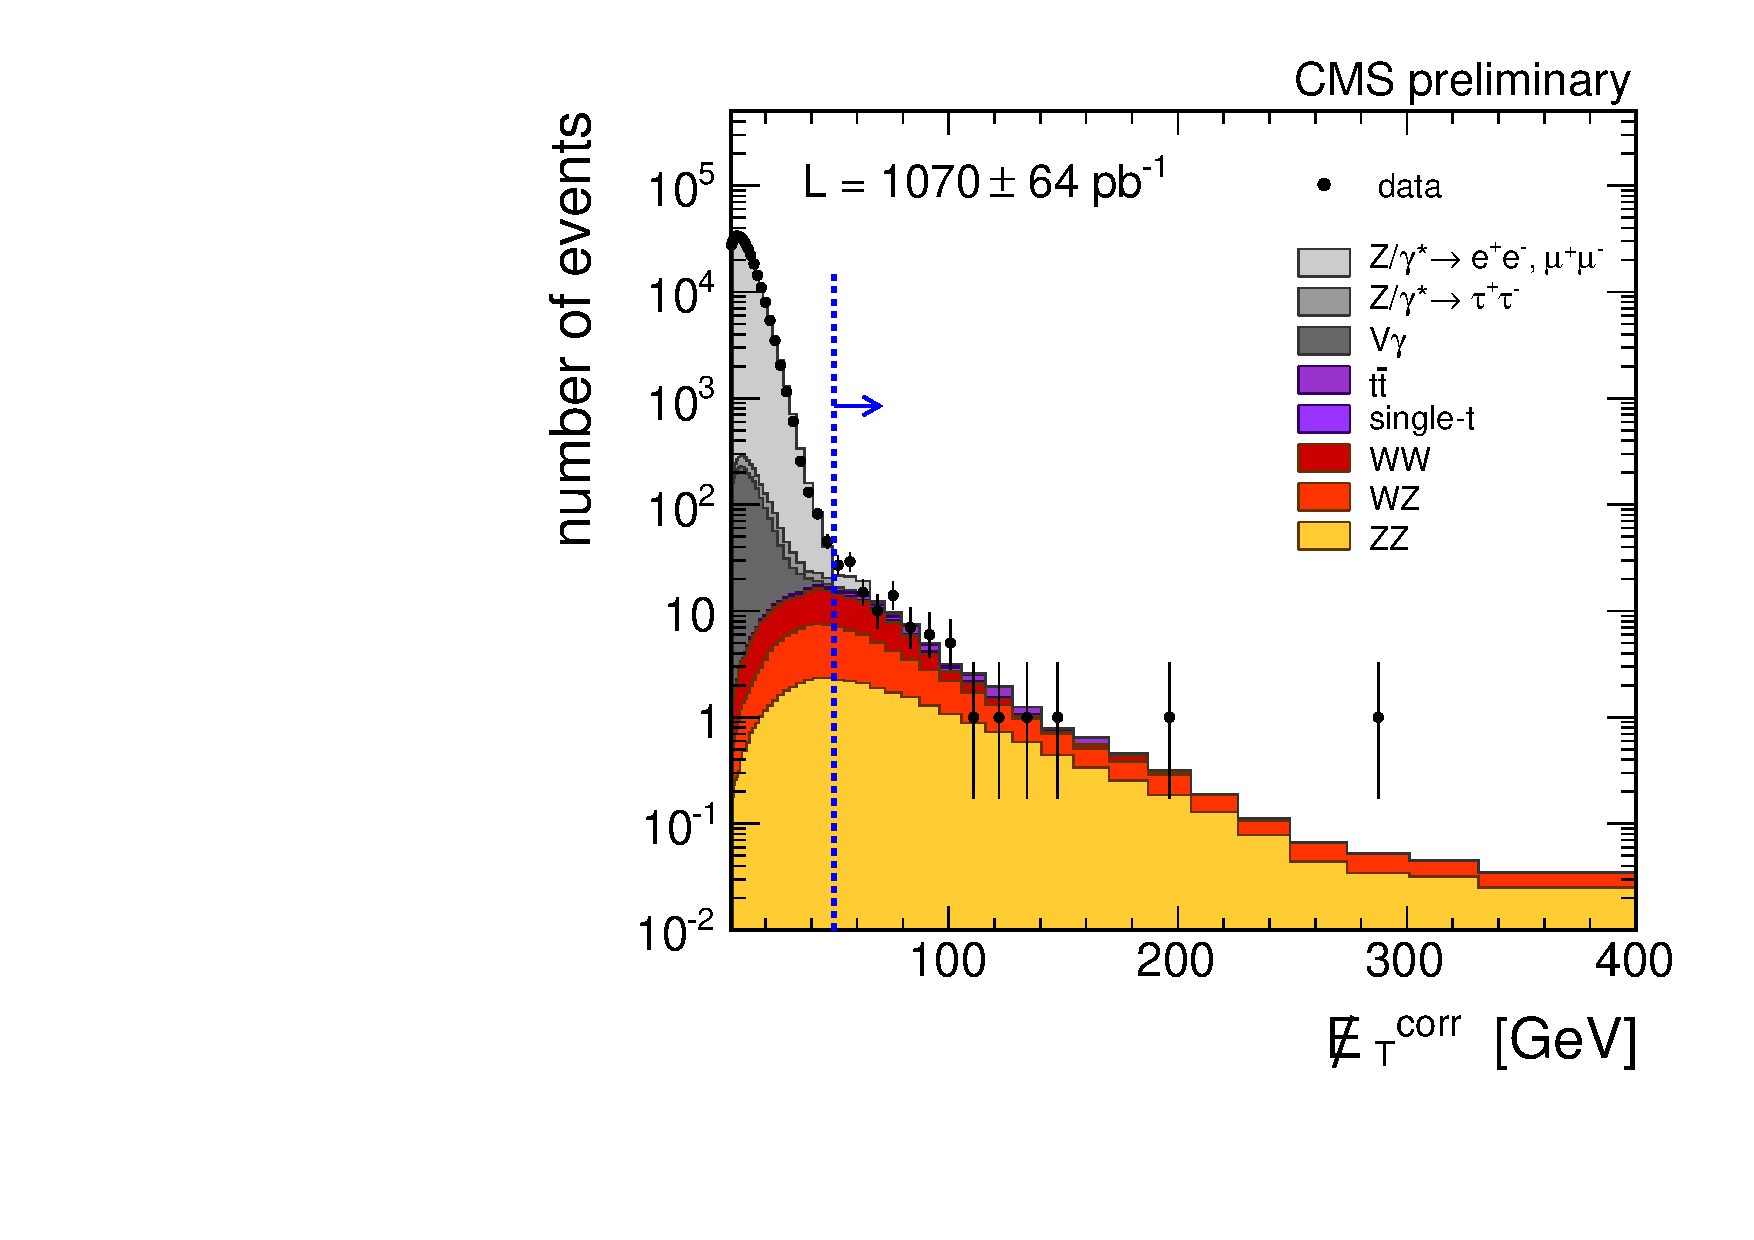
\includegraphics[width=1\linewidth]{figures/ZZ_2l2n/corrMET_jet.pdf}
%\hspace{.05in}
\caption{Distribution of the corrected $\met$ variable for di-lepton events after the jet veto. The cut at $50~\GeV$ is indicated by a dashed blue line. \label{fig:ZZ_2l2n_corrMET_jet}}
%\end{center}
\end{minipage}
\hspace{0.5cm}
\begin{minipage}[t]{0.48\linewidth}
\centering
%\begin{center}
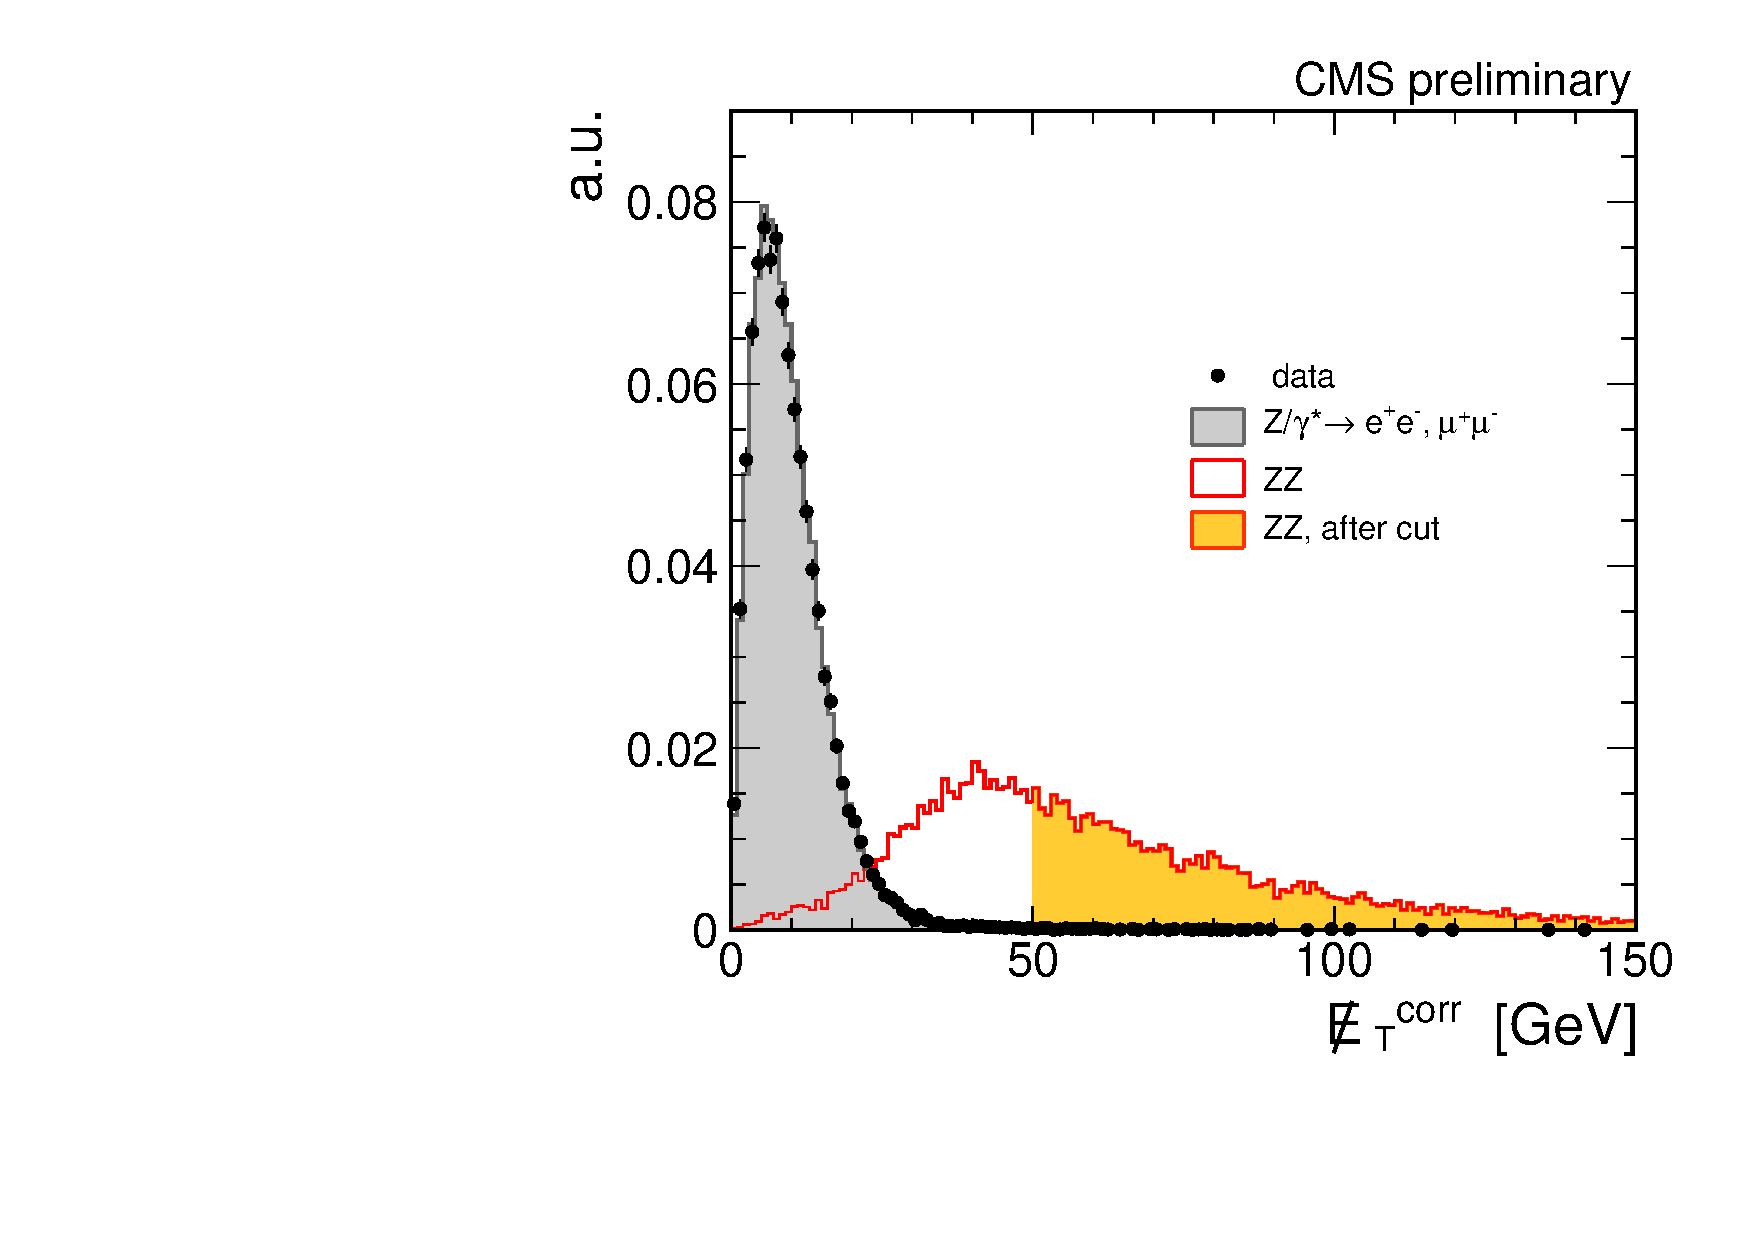
\includegraphics[width=1\linewidth]{figures/ZZ_2l2n/corrMET_q30_jet.pdf}
\caption{Distribution of the corrected $\met$ variable for di-lepton events after the jet veto and the $\QT>30~\GeV$ cut for the data (dots), the Drell Yan simulation (in gray) and the \ZZ\ signal (in red). The distributions are normalized to unity.  \label{fig:ZZ_2l2n_corrMET_q30_jet}}
\end{minipage}
\end{figure}

We consider several missing transverse energy variables. The standard \PFMET\ is constructed as the modulus of $-\Sigma \VECPT$, where the vector sum runs over transverse momenta of calibrated jets and unclustered charged or neutral PF candidates.  In the second variable, called \PUMET, the contribution to the vector sum of objects associated to the pile-up is scaled down by the number of additional vertices. Although the \PUMET\ variable is less sensitive to the conditions of pile-up, it can take erroneously-large values due to possible mis-associations of jets or unclustered PF candidates to the wrong vertices.  To avoid the development of tails in the $\met$ distribution, we form the minimum of the \PFMET\ and \PUMET\ variables. The resulting \PUMETMIN\ variable shows much improved discrimination against the Drell-Yan background compared to the first two variables.  We use a parameterization of the residual dependence of the \PUMETMIN\ variable as a function of the number of additional vertices to obtain a rescaled variable \CORRMET, defined so that the distribution of \PUMETMIN\ for Drell-Yan events in the data without pile-up be unchanged. By construction, a cut on the \CORRMET\ variable presents the same rejection power against Drell-Yan events irrespective of the pile-up conditions, in the electron and muon channels, in the data and the Monte-Carlo simulation.

\begin{figure}[bt]
\begin{minipage}[t]{0.48\linewidth}
\centering
%\begin{center}
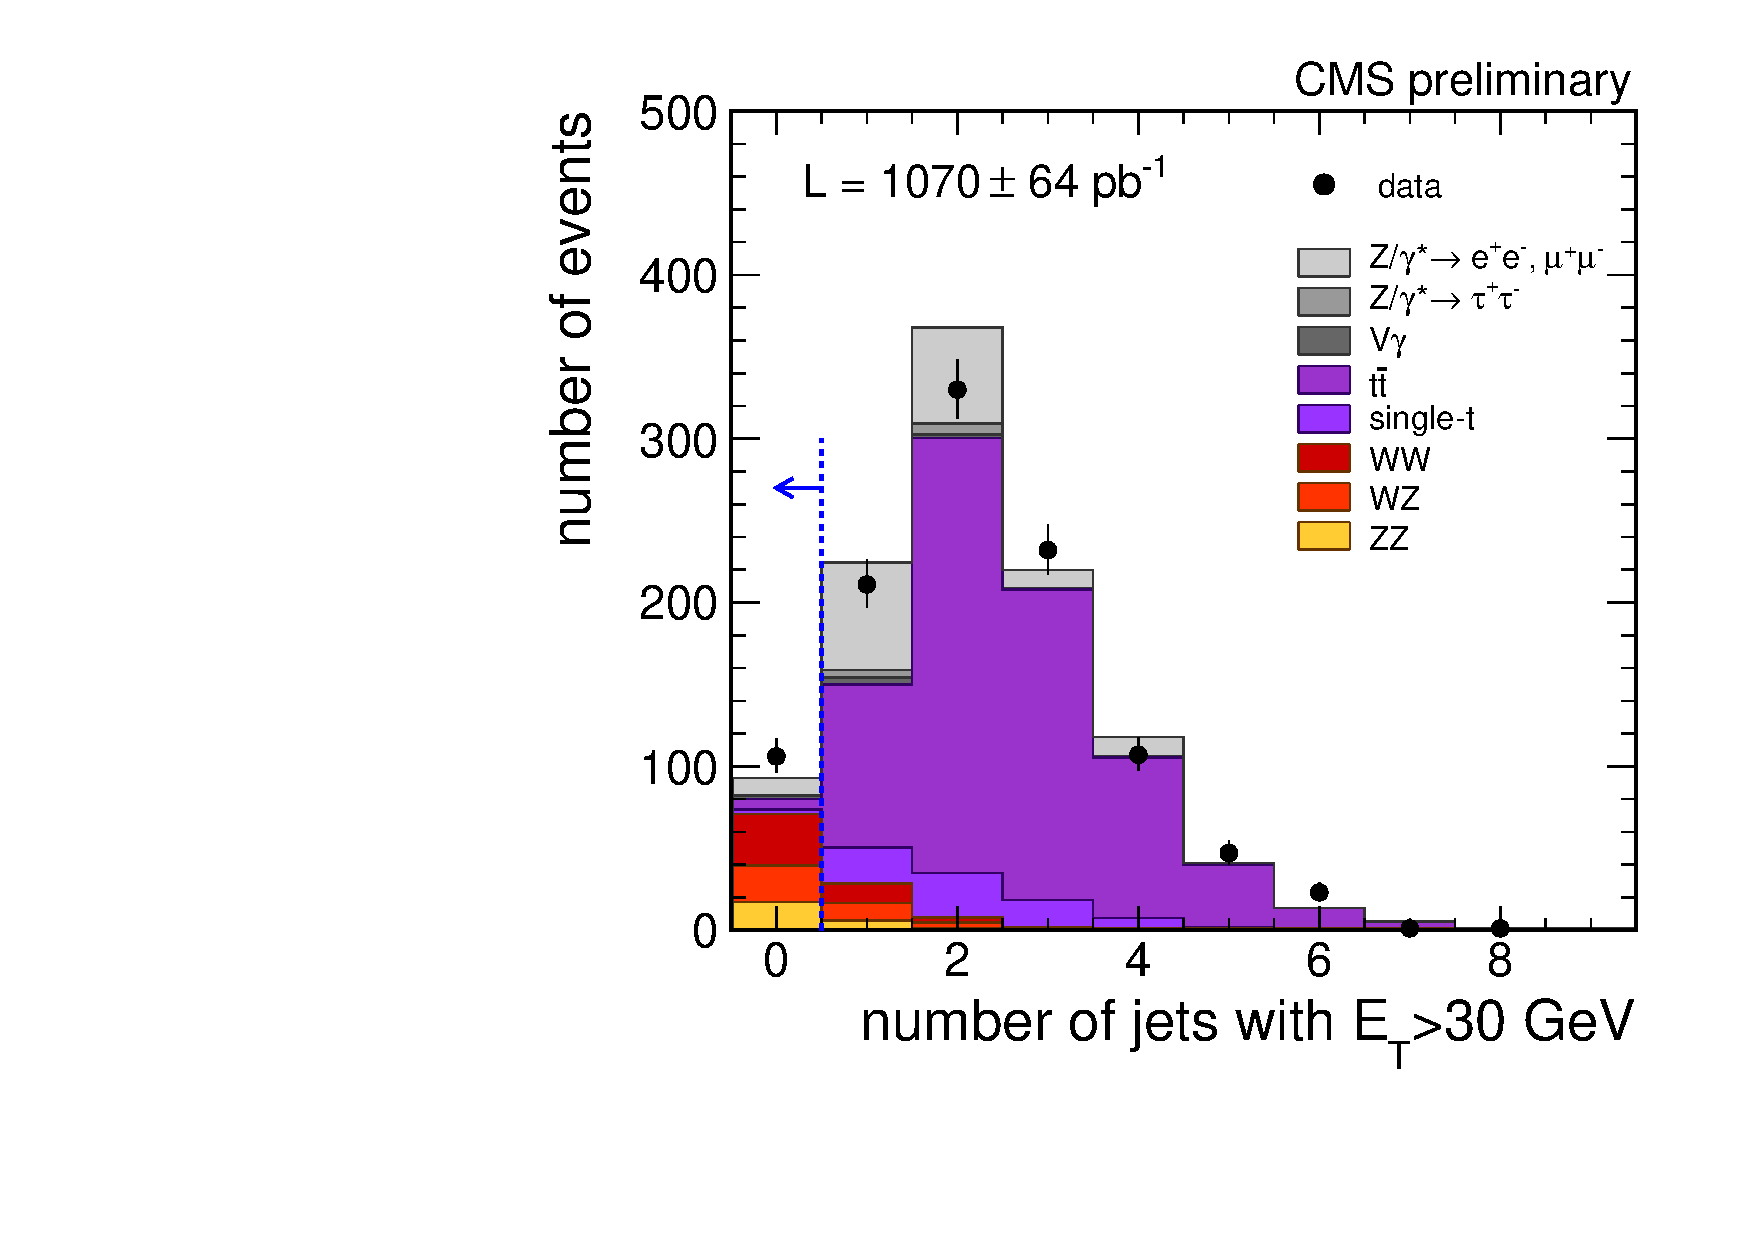
\includegraphics[width=1\linewidth]{figures/ZZ_2l2n/jMult_q30_met.pdf}
\caption{Exclusive jet multiplicity, for di-lepton events after $\QT$ and $\met$ cuts. \label{fig:ZZ_2l2n_jMult_q30_met}}
\end{minipage}
\hspace{0.5cm}
\begin{minipage}[t]{0.48\linewidth}
\centering
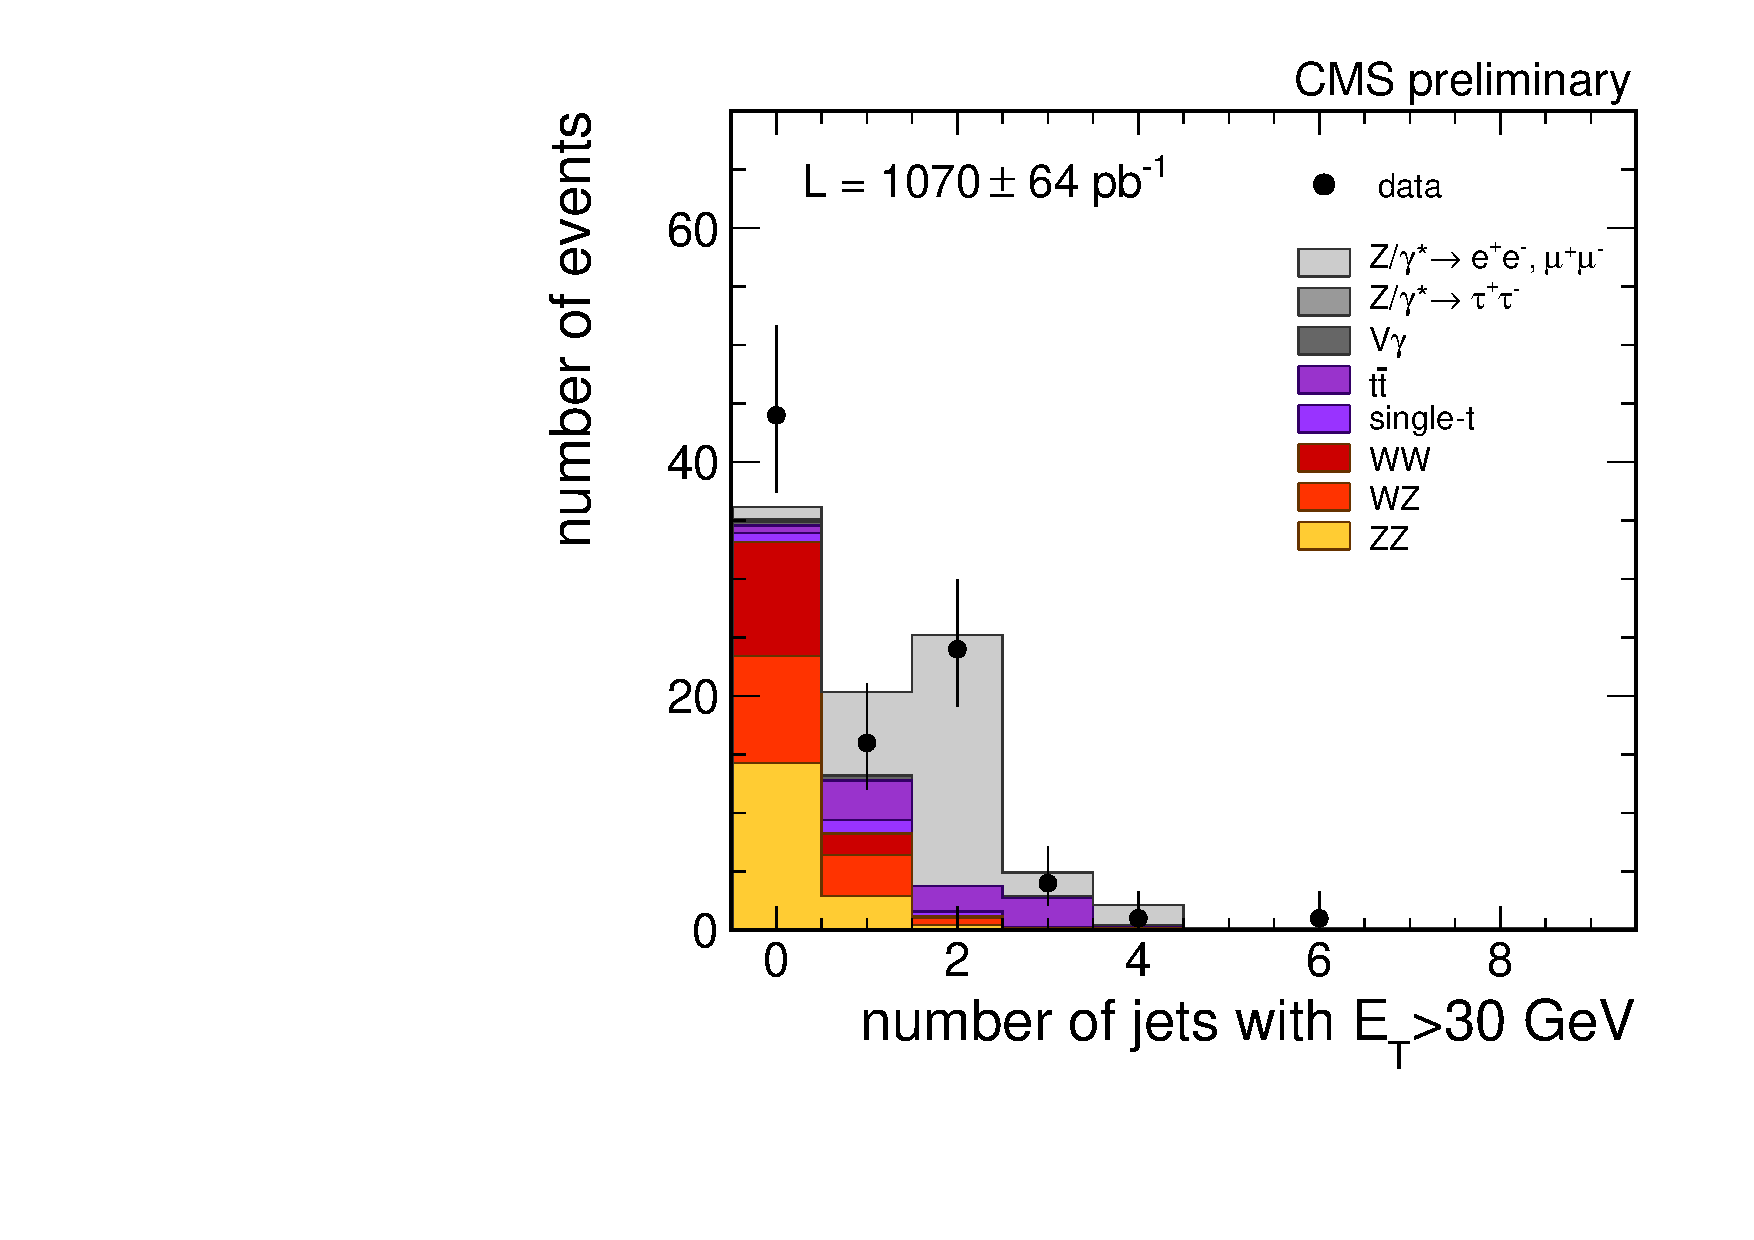
\includegraphics[width=1\linewidth]{figures/ZZ_2l2n/jMult_final.pdf}
%\hspace{.05in}
\caption{Exclusive jet multiplicity, for di-lepton events after all selections, in the $80$-$100~\GeV$ mass window. \label{fig:ZZ_2l2n_jMult_final}}
%\end{center}
\end{minipage}
\end{figure}

To fight the overwhelming $\PZ+{\mathrm {jets}}$ and Drell-Yan backgrounds we apply a jet veto and impose a strong $\met$ requirement. The jet veto energy threshold, $\ET^{\mathrm{jet}}>30~\GeV$, is chosen to stay insensitive to jets originating from pile-up events.  The $\met$ requirement, $\CORRMET>50~\GeV$, is determined to obtain, together with the jet veto, a final rejection factor of $2.5 \times 10^{5}$ against $\PZ+{\mathrm {jets}}$ and Drell-Yan backgrounds.  For convenience, we also apply a cut on the transverse momentum \QT\ of the di-lepton candidate at $30~\GeV$, which is the photon transverse energy threshold of our the $\gamma + \mathrm{jets}$ control sample; this cut has no effect once the jet veto and \CORRMET\ cuts are applied. After the jet veto and the $\QT$ cut, the $\CORRMET>50~\GeV$ cut has an efficiency of $62\%$ on the \ZZ\ signal for an additional rejection of $2\,000$ on the Drell-Yan background. The distribution of the \CORRMET\ variable after jet veto is shown on Fig.~\ref{fig:ZZ_2l2n_corrMET_jet}}, and after the $\QT$ cut on Fig.~\ref{fig:ZZ_2l2n_corrMET_q30_jet}.

The remaining $\PZ+{\mathrm {jets}}$ background is further cleaned-up by three additional kinematical cuts. To ensure the correct  balance between the $\PZ$ boson transverse momentum and the transverse missing momentum we apply a cut on the ratio of the $\MET$ to the di-lepton transverse momentum, $0.4< \MET/\QT < 1.8$, and a cut on the angle between the $\MET$ direction and the di-lepton axis, $\Delta \phi( \MET, -\VECQT )<60^{\circ}$; to reject events with a mismeasured jet we apply a cut on the angle between the $\MET$ direction and the closest jet in the event, $|\min( \Delta \phi ( \MET, { \mathrm{jet} } ) )|>20^{\circ}$. These cuts have close to 100\% efficiency on the signal. 



\begin{figure}[b]
\begin{center}
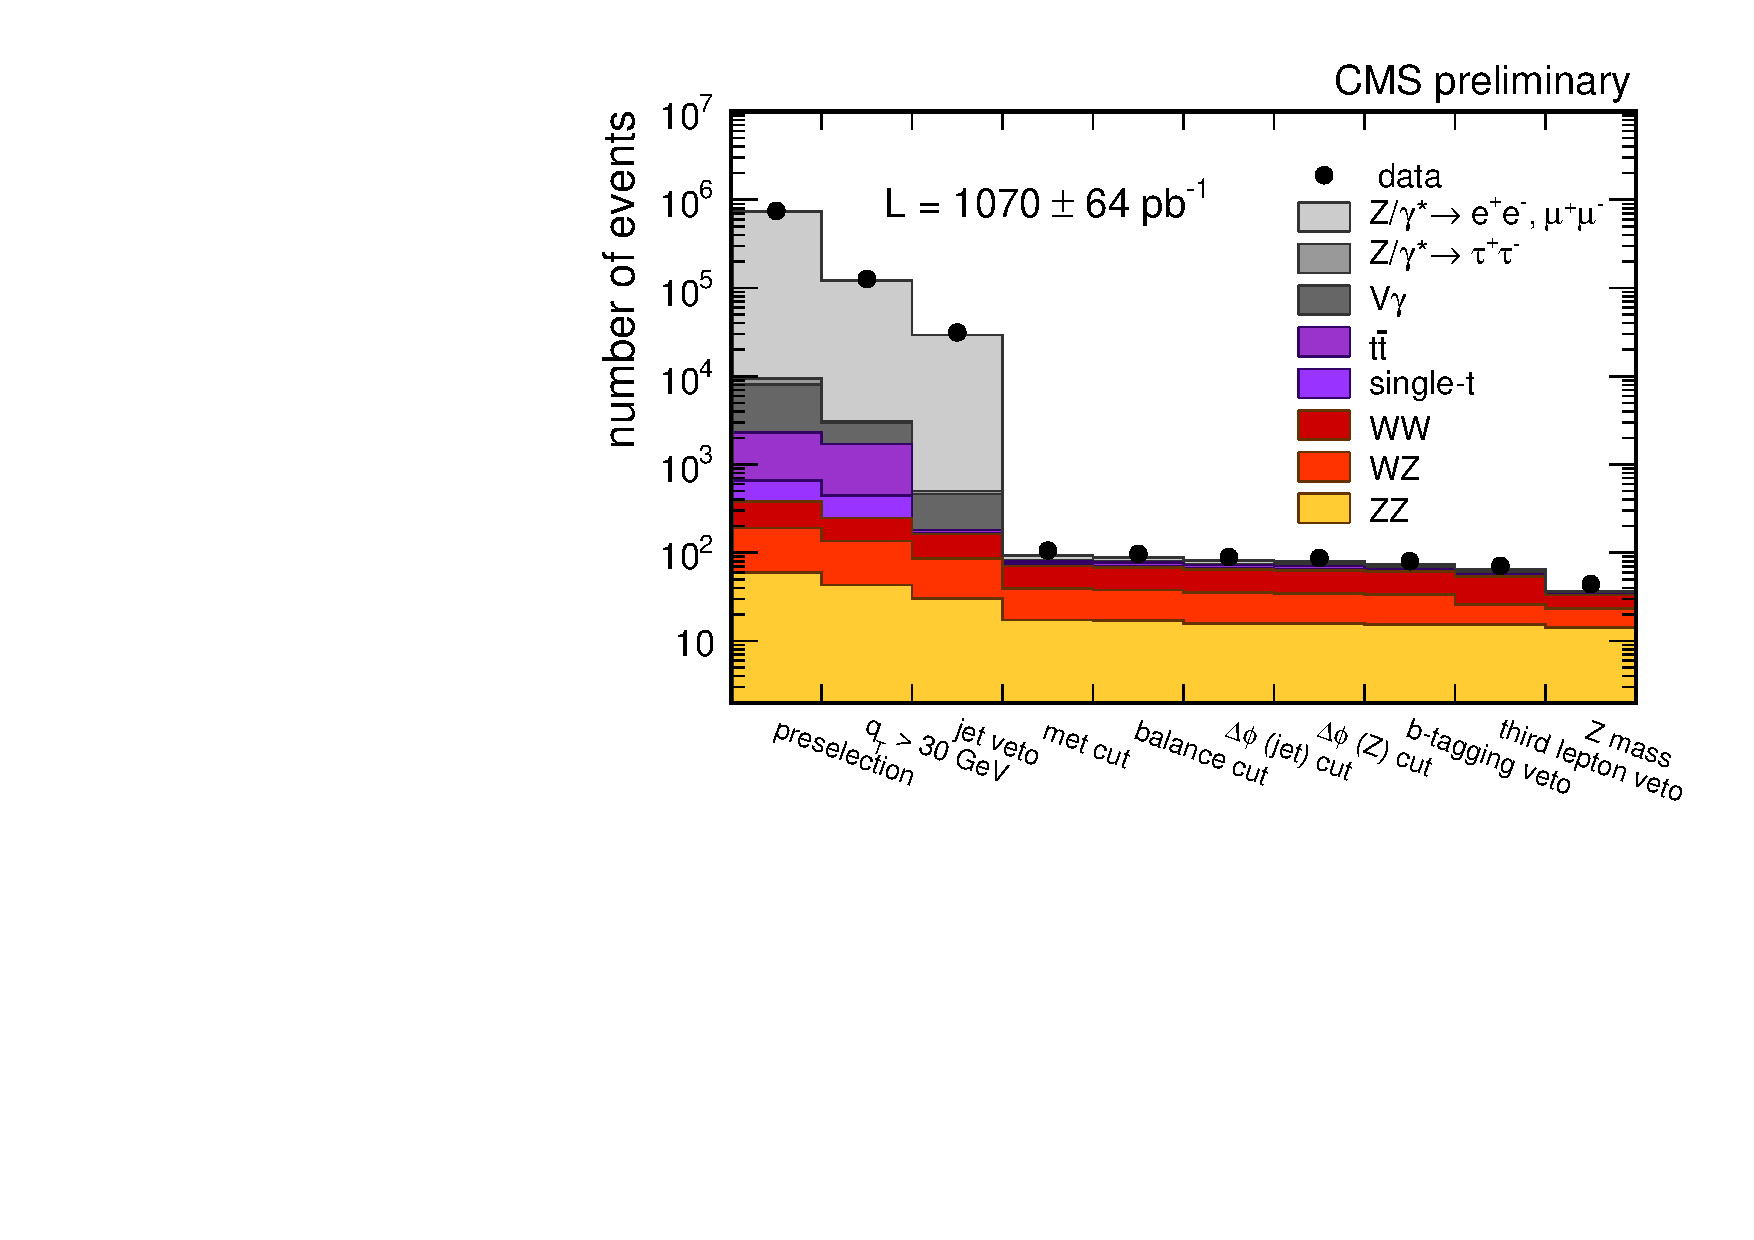
\includegraphics[width=0.70\textwidth]{figures/ZZ_2l2n/Cumul.pdf}
\hspace{.05in}
\caption{Succession of cuts in the $\ZZ\to\ell\ell\nu\nu$ analysis. \label{fig:ZZ_2l2n_cumul}}
\end{center}
\end{figure}


The top backgrounds ($t\bar{t}$ and single-top) are also strongly reduced by the jet veto.  This is illustrated by the jet-multiplicity distribution on Fig.~\ref{fig:ZZ_2l2n_jMult_q30_met}, where only the $\QT$  and the $\CORRMET$ cuts are applied. To further reduce the top backgrounds, we apply a b-tagging veto based on two b-tagging variables, one that counts the number of displaced vertices, another one based on the presence of a soft muon in a jet.  The plot on Fig.~\ref{fig:ZZ_2l2n_jMult_final} shows the jet multiplicity distribution after all kinematical cuts and b-tagging criteria applied, in the reduced $[80$-$100]~\GeV$ mass window. There is good agreement in the 2-jet and 3-jet bins, which are dominated by the $\PZ+\mathrm{jets}$ and top backgrounds, respectively. The agreement is good also in the 1-jet bin, where  $\PZ+\mathrm{jets}$ and top contribute in comparable amount to the background, which represents more than half of the sample. The 0-jet bin is dominated by diboson events, $\WW$, $\WZ$, and $\ZZ$. The $\WZ$ component is reduced by rejecting events containing at least one additional lepton with $\PT>20~\GeV$ selected with looser identification and isolation criteria.  The succession of selection cuts is illustrated on Fig.~\ref{fig:ZZ_2l2n_cumul}.

\begin{figure}[t]
\begin{minipage}[t]{0.48\linewidth}
\centering
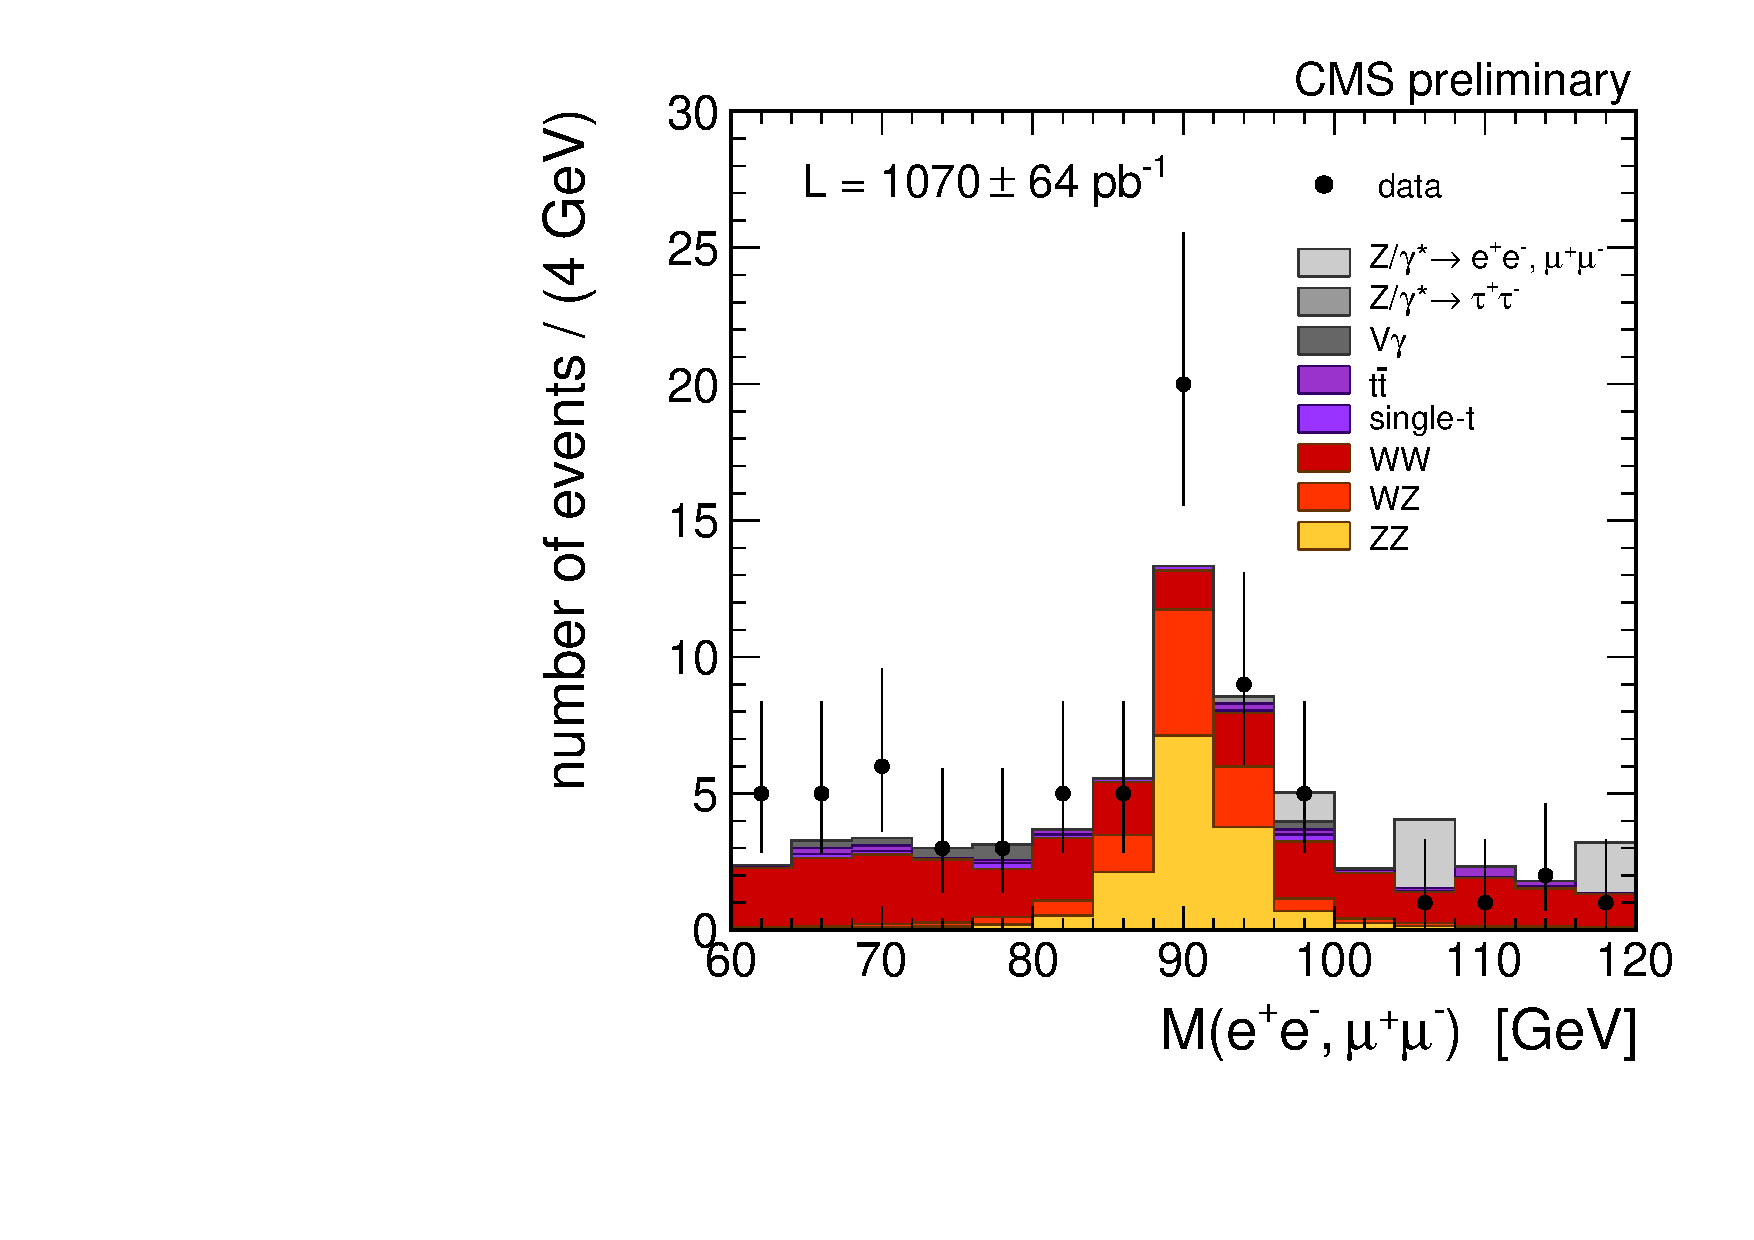
\includegraphics[width=1\linewidth]{figures/ZZ_2l2n/mll_final.pdf}
\caption{Dilepton mass spectrum for the final $\ZZ\to\ell\ell\nu\nu$ selection. \label{fig:ZZ_2l2n_mll_final}}
\end{minipage}
\hspace{0.5cm}
\begin{minipage}[t]{0.48\linewidth}
\centering
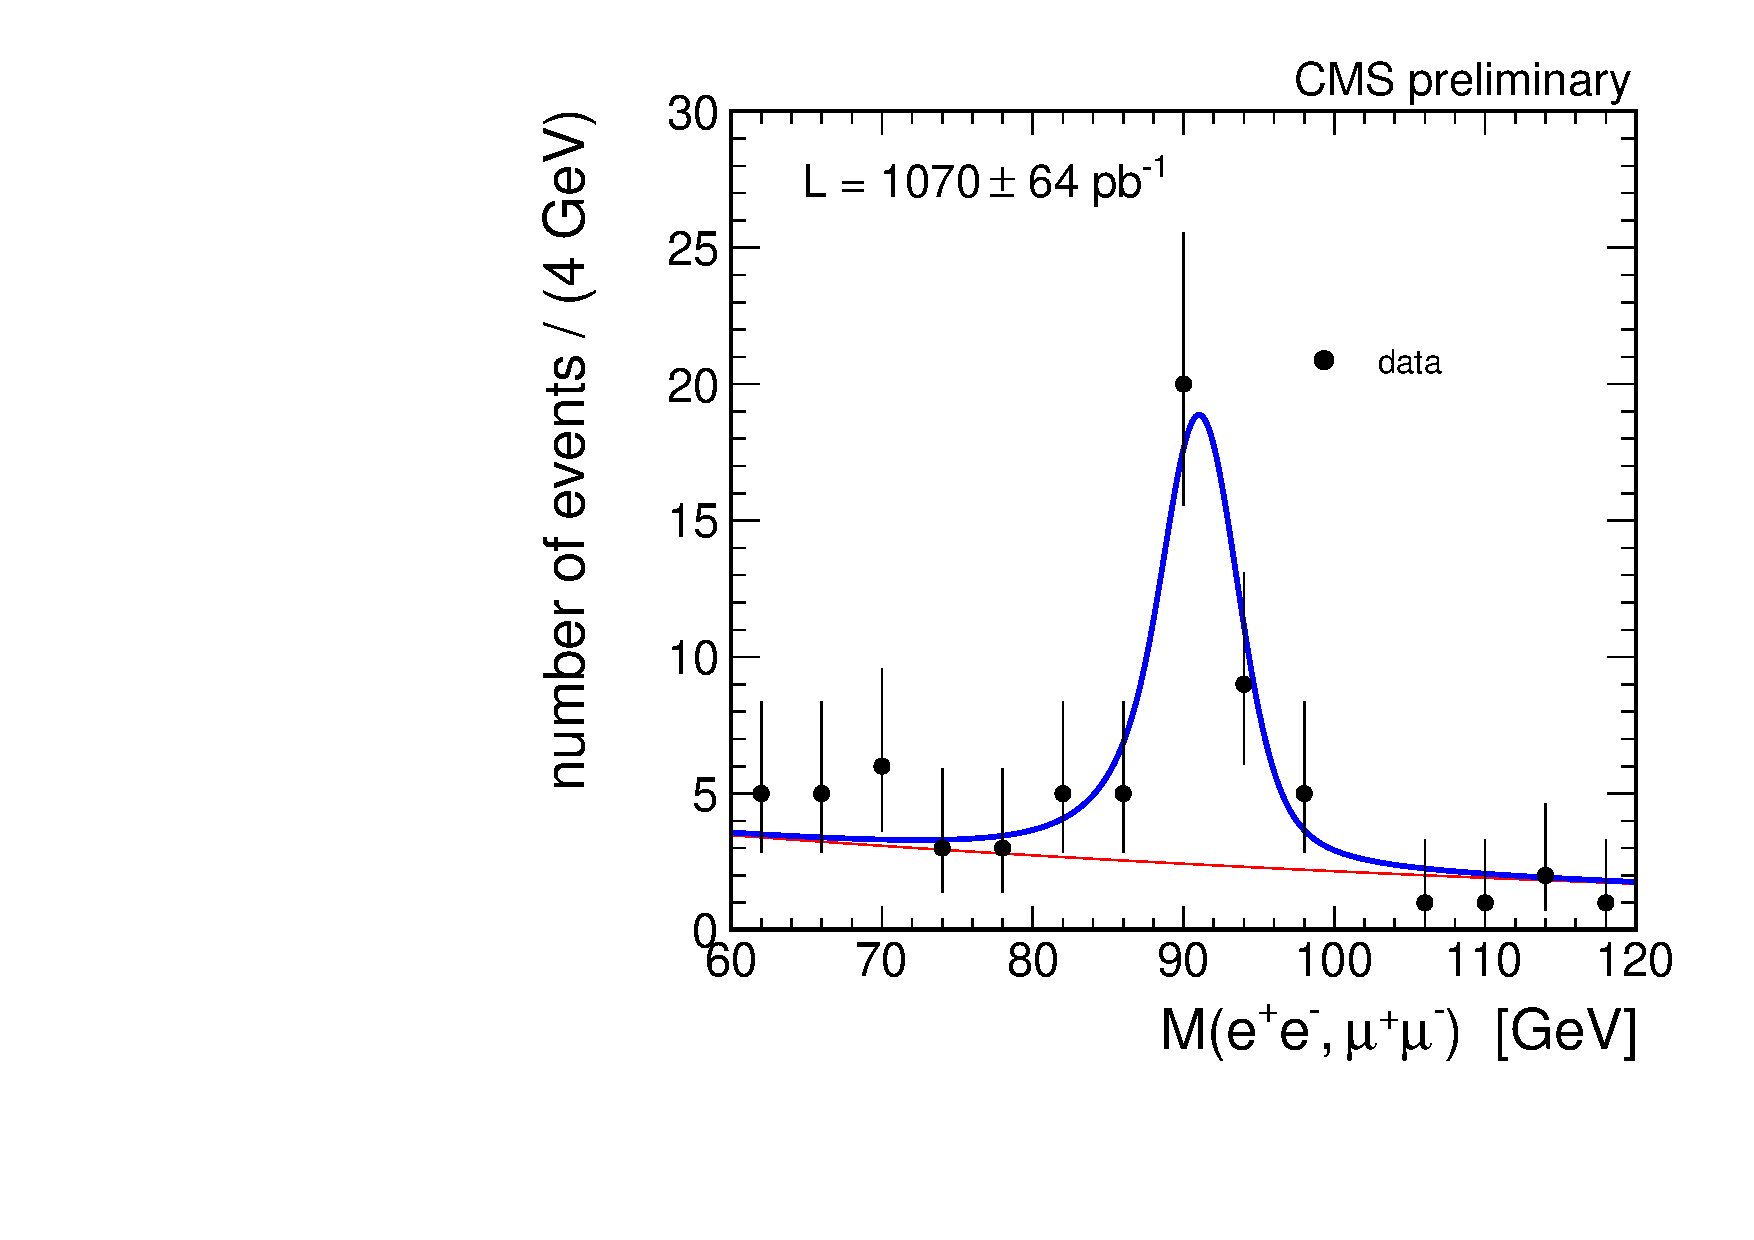
\includegraphics[width=1\linewidth]{figures/ZZ_2l2n/fitMll.pdf}
\caption{Unbinned maximum likelihood fit to the dilepton mass spectrum. \label{fig:mll_fit}}
\end{minipage}
\end{figure}

\def\NELE{\ensuremath{37}}
\def\NELEWIN{\ensuremath{23}}
\def\NMUO{\ensuremath{34}}
\def\NMUOWIN{\ensuremath{21}}

The di-lepton mass spectrum for selected events is shown on Fig.~\ref{fig:ZZ_2l2n_mll_final}.  We select \NELE\ (\NMUO) events in the electron (muon) channel, \NELEWIN\ (\NMUOWIN) of which in the reduced $[80$-$100]~\GeV$ mass window. The Monte Carlo simulation for the $\WW$, $\WZ$ and $\ZZ$ components are produced at the leading order (LO) in QCD with the Pythia event generator; a dynamical NLO/LO weight (k-factor), determined using NLO and LO differential cross-sections computed with MCFM, is applied event-by-event.  

We use an unbinned maximum likelihood fit to the di-lepton spectra to extract the peaking component and the non-peaking \WW\ background. In the fits, the \PZ\ line-shape comes from a $\PZ+\mathrm{1\,jet}$ control sample in the data, described later, and the \WW\ line-shape, from the Monte-Carlo simulation. Other non-peaking backgrounds are taken as uniform in the mass window, except for the $\PZ\to\tau^+\tau^-$ background, which found to be negligible. Because the \PZ\ line-shapes differ in the electron and muon channels due to different mass resolution functions, the fits are performed separately.  Figure~\ref{fig:mll_fit} is an illustration of a fit to the combined lepton sample using an averaged \PZ\ line-shape.   

%\begin{figure}[hbt]
%\begin{center}
%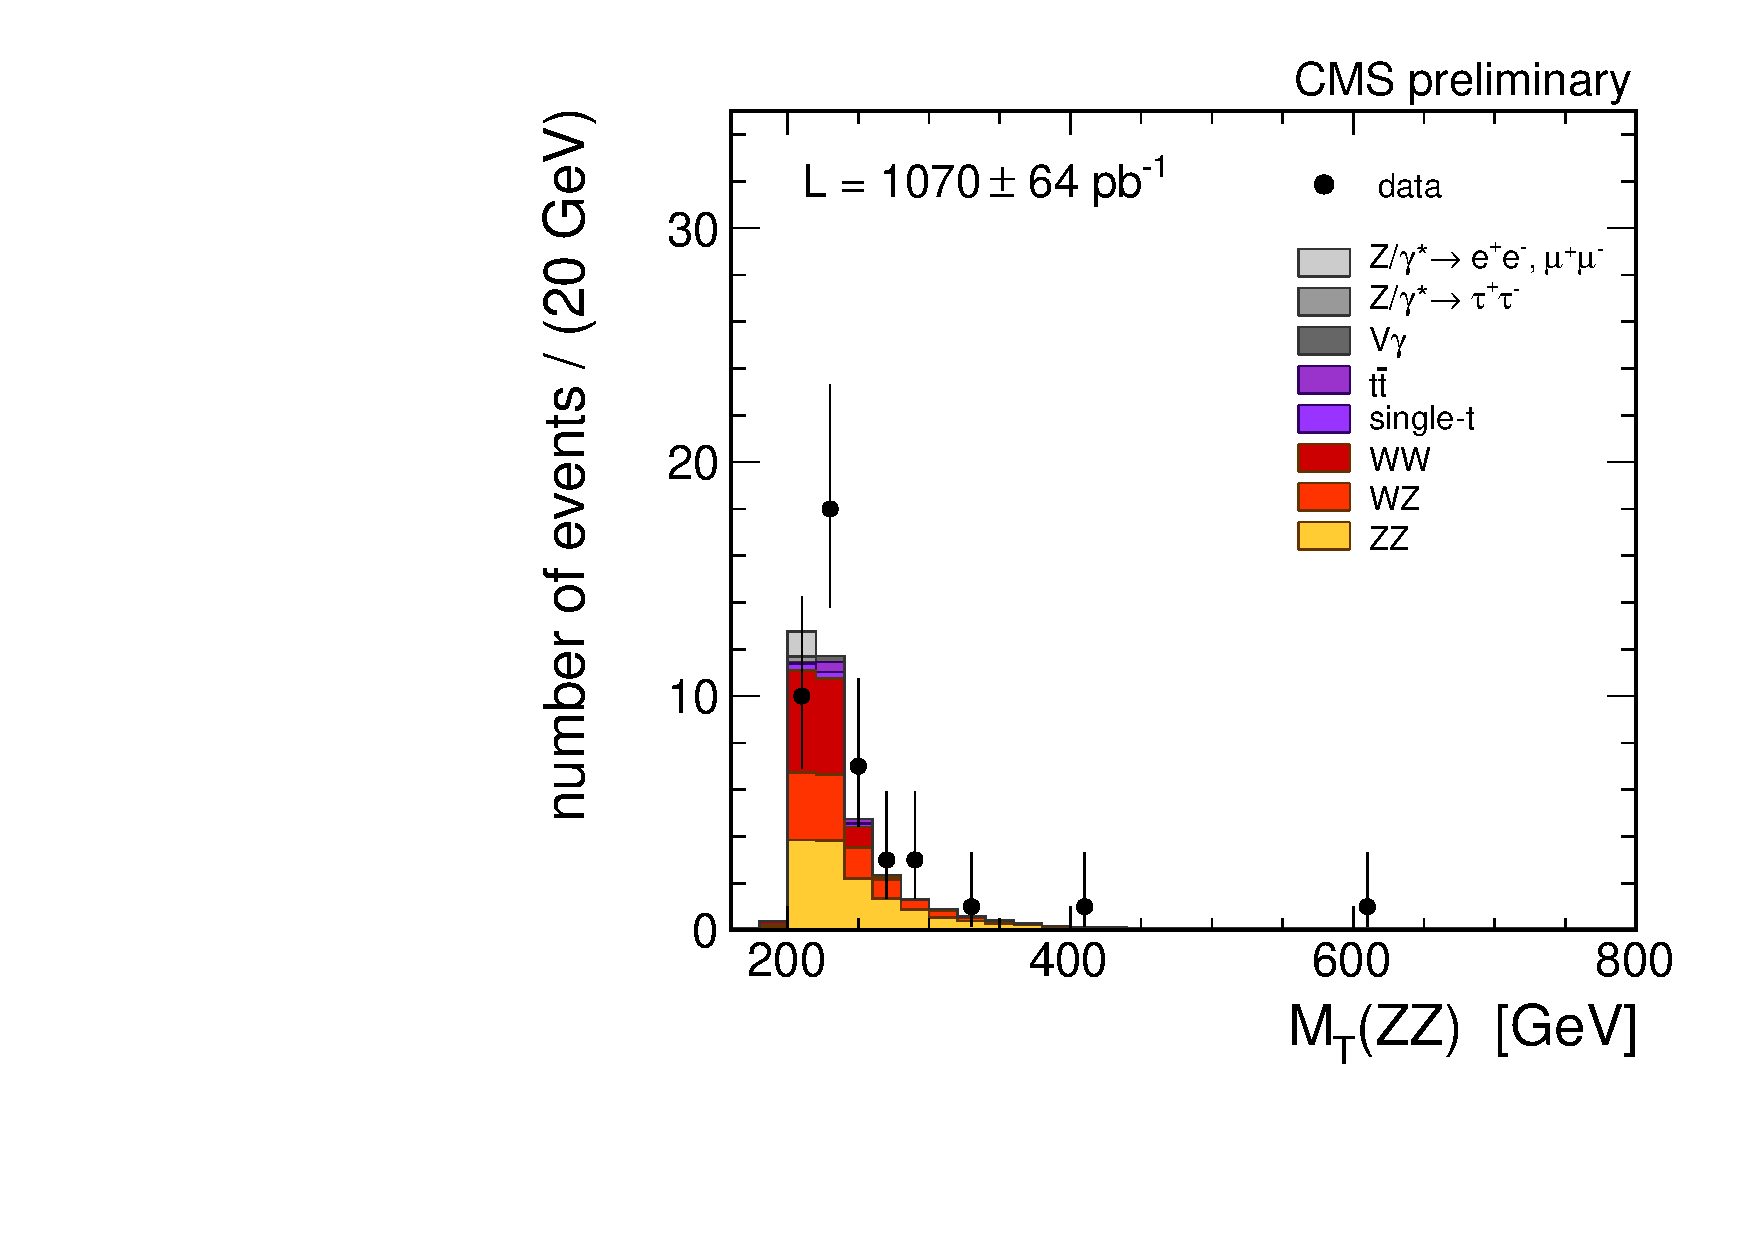
\includegraphics[width=0.70\textwidth]{figures/ZZ_2l2n/mTZZ_final.pdf}
%\hspace{.05in}
%\caption{$ZZ$ transverse  mass for the final $\ZZ\to\ell\ell\nu\nu$ selection in the $[\,80\,$-$\,100\,]~\GeV$ mass window. \label{fig:ZZ_2l2n_mTZZ_final}}
%\end{center}
%\end{figure}

%The $(\PZ,\met)$ transverse mass distribution for the 14 events in a restricted $[\,80\,$-$\,100\,]~\GeV$ di-lepton mass window around the $Z$ peak (9 and 5 in the electron and muon channels, respectively) is shown in Fig.~\ref{fig:ZZ_2l2n_mTZZ_final}.  The level of Drell Yan, $\PZ+{\mathrm{jets}}$, $Z\to\tau\tau$ and $\PW+{\mathrm{jets}}$ backgrounds is expected to be negligible from the simulation.  The background of $t\bar{t}$ events is estimated at $0.5\pm0.3$ where the error comes from the Monte Carlo statistics. The expected number of diboson events in the restricted mass window is 3.2, 4.1 and 6.5 for the $\WW$, $\WZ$ and $\ZZ$ modes, respectively.  

\subsection{Backgrounds}

Most considered backgrounds are estimated or cross-checked using data-driven methods. 

The $\PW+\mathrm{jets}$ background is estimated using a method where the electron fake rate is measured from loose electron candidates in a pure QCD background sample, and applied to a sample of $\PZ$ candidates with one loose electron candidate. The $\PW\gamma$ background is estimated from simulation. We check that adding photon conversion rejection requirements to the electron identification criteria has no impact on the selected sample. These backgrounds are found to contribute only to the non-peaking background in the electron channel: $3.5\pm1.6$ and $1.5\pm0.5$ events for $\PW+\mathrm{jets}$ and $\PW+\gamma$, respectively. 

The $\PZ\gamma\to\ell^+\ell^-\gamma$ background, where one of the leptons falls outside acceptance, is negligible in the muon channel and very small in the electron channel. Events with both leptons in acceptance and surviving all the cuts, contribute to the peaking background. This contribution is estimated from the Monte-Carlo simulation: $0.3\pm0.2$  ($0.1\pm0.1$) events in the electron (muon) channels, with large errors.  

The top background is estimated from the centrally measured b-tagging efficiency and the fraction of events rejected by our b-tagging requirements in a top-enriched control sample obtained by inverting the di-lepton mass window and requiring at least two hard jets in the event. The top contribution to the non-peaking background amounts to $0.7\pm0.4$ and $1.0\pm0.5$ events in the electron and muon channels, respectively. 

The Drell-Yan background is estimated by extrapolating the \CORRMET\ distribution from the Drell-Yan dominated region to the signal region. The functional form of the \CORRMET\ distribution for the Drell-Yan is exercised on the Monte-Carlo simulation (we adopt a three-parameter Novosibirsk function), fitted on the data below $30~\GeV$ and integrated above the cut value of $50~\GeV$. We obtain $3.6\pm0.9$  and $1.6\pm0.4$ events in the electron and muon channels, respectively. We cross-check the contribution of Drell-Yan and $\PZ + {\mathrm {jets}}$ backgrounds using a sample of QCD events in the data containing one hard isolated photon with $\ET^{\gamma}>30~\GeV$.  Photons are selected with very tight identification and isolation criteria to get a reasonable photon purity. We apply the jet veto and we re-weight the events in the control sample so that the photon transverse momentum spectrum matches that of the $\PZ$ boson. We then normalize the $\CORRMET$ distribution of the $\gamma+\mathrm{jets}$ sample to that of the $\PZ + {\mathrm {jets}}$ in a region around the maximum of the distribution. The contribution of $\PZ\gamma \to \nu\nu\gamma$ events, which dominates the tails of the $\CORRMET$ distribution in the control sample, is estimated from the Monte-Carlo simulation normalized to the CMS measurement of the $\PZ\gamma$ production cross-section, and subtracted. The experimental error of $40\%$ on the $\PZ\gamma$ cross-section is propagated to the final background estimates. 
We obtain background estimates that are consistent, within errors. The $\gamma+\mathrm{jets}$ control sample ensures that there is no unexpected source of tails in the \CORRMET\ distribution. 

The background-subtracted \WZ/\ZZ\ yields are $${N^{\WZ/\ZZ}}_{\Pe}=\NElePeakingWithWZ\ \ \mathrm{and}\ \ {N^{\WZ/\ZZ}}_{\Pgm}=\NMuoPeakingWithWZ,$$
and the background-subtracted \WW\ yields are $${N^{\WW}}_{\Pe} = \NEleNonPeaking\ \ \mathrm{and}\ \ {N^{\WW}}_{\Pgm}=\NMuoNonPeaking,$$ in the electron and muon channels, respectively.

%We can then compare, on both samples, the effect of the $\CORRMET$ and other kinematical cuts.  

\subsection{Efficiencies}

The values of di-lepton selection efficiency ${(\mathcal{A}\times\varepsilon)^{\ZZ\,(\WZ)}}_{\ell\ell}$, determined from the simulated \ZZ\ (\WZ) samples with dynamical NLO/LO re-weighting, are  $39.6\%$ ($36.7\%$) and $58.2\%$ ($53.3\%$) in the electron and muon channels, respectively. The values of ${(\mathcal{A}\times\varepsilon)^{\ZZ\,(\WZ)}}_{\ell,\mathrm{sim}}$ after all selections are obtained from the simulation with a dynamical NLO/LO re-weighting that takes into account the effect of the jet veto on the NLO cross-sections. We find $8.5\%$ ($2.0\%$) and $11.0\%$ ($2.8\%$) for the \ZZ\ (\WZ) mode in the electron and muon channels, respectively. 

We use ratios of efficiencies on control samples in the data and the simulation, $\rho = \epsilon_{\mathrm{data}}/\epsilon_{\mathrm{sim}}$, as signal efficiciency correction factors, $\varepsilon = \rho \times \varepsilon_{\mathrm{sim}}$. 

The correction factors for lepton trigger, reconstruction, identification and isolation are determined by the tag-and-probe method. The largest correction is in the electron channel, $\rho=0.931\pm0.002$.  The di-lepton trigger efficiencies are estimated assuming that the lepton trigger efficiencies factorize: $98.8\pm0.3\%$ and $92.2\pm0.1\%$ for di-electron and di-muon triggers, respectively.  The tag-and-probe results are also exploited to correct the third-lepton veto efficiency on the \WZ\ sample, $\rho=1.015\pm0.009$. 

We use the ratio of jet-veto efficiencies on $\PZ+\mathrm{jets}$ samples in the data and the NLO simulation to correct the jet veto efficiency on the \ZZ\ and \WZ\ simulated samples. We check the validity of the method by applying it to a $\PZ+\mathrm{jets}$ sample generated at the LO with Pythia, and by varying the jet-veto threshold. The same control sample with a $\met$ cut is exploited to determine the b-tagging veto efficiency on non-top events, $\sim95\%$ with a correction factor consistent with one. The third-lepton veto efficiency on \ZZ\ events, close to 100\%, does not need correction.  

For the study of the \CORRMET\ and the three kinematical cuts, we construct a control sample from the sample of \PZ\ events with $\QT>30~\GeV$ and exactly one jet of transverse energy larger than $30~\GeV$. 
%As described above, this jet is attributed to the hard-scatter vertex; therefore, its contribution is not scaled down in the computation of the \PUMET\ variable.  
We ignore the jet in the computation of the \PUMET\ variable and in the jet veto as if the jet went undetected, and we re-weight events to match the \PZ\ transverse momentum spectrum of the \ZZ\ signal.  
%We do so in the data and in the Monte-Carlo simulation and we use 
Data/simulation efficiency ratios are then obtained for the \CORRMET\ and kinematical cuts, 
applied one after the other. 
The largest discrepancy ($\rho\sim0.75$) is found for the \CORRMET\ cut. This results from the imperfect modeling of the off-time pile-up in the simulation; the scaling involved in the computation of the \CORRMET\ variable has an impact on events with genuine missing transverse energy that is larger in the data than in the simulation. We check this assumption by performing the analysis with the un-scaled \PUMETMIN\ variable instead of \CORRMET. To obtain the same rejection factor on the Drell-Yan background,  the cut on \PUMETMIN\ must be placed $15~\GeV$ higher in the data, which leads indeed to a consistent relative loss of signal efficiency.   The di-lepton spectra obtained at the end of the selection on these control samples in the data provide the \PZ\ line-shapes for the unbinned maximum likelihood fits.   

The overall efficiency correction factors are, for the \ZZ\ mode, 
$${\rho^{\ZZ}}_{\Pe}=\RhoEleZZ\ \ \mathrm{and}\ \ {\rho^{\ZZ}}_{\Pgm}=\RhoMuoZZ,$$
and, for the \WZ\ mode,
$${\rho^{\WZ}}_{\Pe}=\RhoEleWZ\ \ \mathrm{and}\ \ {\rho^{\WZ}}_{\Pgm}=\RhoMuoWZ,$$
in the electron and muon channels, respectively.

The numbers of \WZ\ events are estimated using the CMS results on \WZ\ in the $3\ell\nu$ channel described in Ref.~\cite{CMS-PAS-EWK-11-010} and the ${(\mathcal{A} \times \varepsilon)^{\WZ}}_{\ell,\mathrm{sim}} \times {\rho^{\WZ}}_{\ell}$ products. We find $ {N^{\WZ}}_{\Pe} = \NbkgZWInZZee $ and $ {N^{\WZ}}_{\Pgm} =  \NbkgZWInZZmm$ in the electron and muon channels, respectively. We obtain consistent but less precise results from the numbers of events rejected by the third lepton veto.

%All other selection cuts have no impact on the signal efficiency, and therefore lead to negligible systematic uncertainties. 

\subsection{Production Cross-Sections}

The production cross-section times branching ratio measurements are based on the equation 
$$
   \SIGBRZZll = \frac{{N^{\WZ/\ZZ}}_{\ell} - {N^{\WZ}}_{\ell} }{ {(\mathcal{A} \times \varepsilon)^{\ZZ}}_{\ell,\mathrm{sim}} \times {\rho^{\ZZ}}_{\ell} \times \mathcal{L} }\ \, , 
$$
with $\ell=\Pe$ or $\ell = \Pgm$. We measure
\begin{eqnarray}
  \SIGBRZZee &=& \ZZElecXsect , \nonumber \\
  \SIGBRZZmm &=& \ZZMuonXsect , \nonumber 
\end{eqnarray}
and, for the combined lepton channel, 
\begin{eqnarray}
  \SIGBRZZll &=& \ZZCombXsect  , \nonumber
\end{eqnarray}
with $\ell$ denotes either electron or muon. 

Using the known branching fractions of the \PZ\ boson we obtain a measurement of the $\pp \to \ZZ $ inclusive production cross-section, 
\begin{eqnarray}
  \SIGZZ &=& \ZZXsect \, .\nonumber
\end{eqnarray}

This result is in agreement with the Standard Model expectation, $\sigma( \pp \to \ZZ ) = 5.9~\mathrm{pb}^{-1}$, computed at the next-to-leading order in perturbative QCD with the MCFM program.

\subsection{Systematic Uncertainties}

\def\GlobSystElec{ \ensuremath{ 18.9\%  }\xspace}
\def\GlobSystMuon{ \ensuremath{ 16.2\%  }\xspace}
\def\GlobSystComb{ \ensuremath{ 17.6\%  }\xspace}

We hereby mention only the main source of systematic uncertainties.

The uncertainties on di-lepton acceptance due to parton density functions are estimated at the 90\% confidence level with the latest MSTW-LO PDF set and lead to a relative uncertainty of $1.5\%$ on the cross-section measurements.  The electron and muon energy/momentum scales induce relative selection uncertainties of $2(3)\%$ for electrons in the EB (EE) and $3\%$ for muons, which propagate to a relative uncertainty of $1.5\%$ on the cross-section measurements.  Uncertainties on lepton reconstruction, identification and isolation efficiency correction factors from the tag-and-probe are propagated to the cross-section measurements. 

The jet veto efficiency depends on the jet energy scale, which is known to $3\%$ at the veto threshold $\ET=30~\GeV$. This translates to a $3.4\%$ uncertainty on the jet veto efficiency, which in turn propagates as a \JVUncEffect relative uncertainty on the cross-section measurements. An additionnal uncertainty of $0.6\%$ is assigned to the jet veto efficiency correction factor obtained from the $\PZ+\mathrm{jets}$ control sample.

The missing transverse energy requirement is an important source of systematic uncertainty on the signal selection efficiency.  We do not correct for the difference in efficiency of the \CORRMET\ cut on the \ZZ\ signal and the $\PZ+1$-jet control sample in the simulation, which is 8.8\%, because part or all of the difference may be of physical origin, but we take it as a systematic uncertainty.  We also take the variation of signal efficiency between two samples reconstructed with a difference of two pile-up vertices around the average as a systematic uncertainty. The total systematic uncertainty due to the \MET\ requirement is 11.9\%. 

The peaking backgrounds are major sources of uncertainty on the cross-section measurements.   The relative uncertainties on the Drell-Yan background are $28\%$ and $25\%$ for the electron and muon channels, respectively, translating into about $6\%$ on the cross-section measurements. The relative uncertainties on the \WZ\ measurements propagated to the cross-sections amount to $4.4\%$ and $5.8\%$, respectively. The total uncertainties due to peaking backgrounds are $14.3\%$ and $10.6\%$, respectively. The uncertainties on non-peaking backgrounds have little impact on the final cross-section results. 

The systematics uncertainties are added in quadrature to give an overall uncertainty of \GlobSystElec\ for the electron channel, \GlobSystMuon\ for the muon channel and \GlobSystComb\ for the combined lepton channel.

The relative uncertainty on the luminosity is estimated to 6\% for the present 2011 data set.

\subsection{Limits on Anomalous Triple-Gauge Couplings}

The \ZZ\ production process provides a way to probe the neutral trilinear gauge couplings at the ZZZ and $\ZZ\gamma$ vertices, which are forbidden at the tree level in the Standard Model.

The neutral trilinear gauge couplings are modelized in an effective Lagrangian by operators, each associated to an anomalous coupling constant.  It is usual to consider two coupling constants for each $\PZ\PZ\PV$ vertex,  $f_{4}^{\PV}$ and $f_{5}^{\PV}$ where $\PV = \PZ,\, \gamma$, associated to operators that are invariant or not under CP symmetry, respectively.  The presence of anomalous couplings modifies the boson spectrum at large transverse momenta, as illustrated on Fig.~\ref{fig:ZZZaTGC_ZPt}, and results in general in an enhancement of the total diboson production cross-section.  We hereby establish limits on a possible enhancement of the total production cross-section given the observations, and translate these limits into contours in the space of the $f_{4}^{\PZ}$ and $f_{5}^{\PZ}$ anomalous coupling constants.

Limits on a possible enhancement of the total cross-section are computed using an hybrid frequentist/Bayesian approach. The null hypothesis $H_0$  corresponds to the Standard Model prediction; the alternate hypothesis $H_1$, to an anomal \ZZ\ production cross-section. Let $r$ be the ratio of the enhanced to the SM-expected cross-sections.  We construct a test-statistics $\mbox{LLR}=-\ln{Q}$, where $Q$ is the likelihood ratio for null over alternate hypotheses. The likelihood functions are Poisson probabilities of observing the actual number of events under the given hypothesis. Sources of systematic uncertainties are considered as nuisance parameters that are integrated out assuming log-normal priors. 

Large numbers of pseudo-experiments are generated to determine the distributions of the test statistics $\mbox{LLR}$ for given values of $r$.  The consistency with the Standard Model is measured as the probability $P_0$ to obtain $\mbox{LLR}>0$ for $r=1$. The inconsistency with the Standard Model for a given value of $r>1$ is measured as the probability $P_1(r)$ to obtain $\mbox{LLR}<0$. Let $\alpha$ be the considered confidence level.  The limit with confidence level $\alpha$ is defined as the smallest value of $r$ for which the ratio $P_1/P_0$ equals $1-\alpha$.  

We obtain limits of $2.3$ and $1.6$ on the $r$ parameter at the  $95\%$ and $68\%$ confidence level, respectively. These values are used to set limits on anomalous triple gauge parameters $f_{4}^{\PZ}$ and $f_{5}^{\PZ}$. For each point in the ($f_{4}^{\PZ},f_{5}^{\PZ}$) plane we determine the value of $r$ by re-weighting the selected \ZZ\ events from the simulation according to the invariant mass of the \ZZ\ system. Weights are computed using the Baur generator with no energy-dependent form factor.  The regions consistent with our limits on $r$ are delimited by the approximate ellipses shown on Fig.~\ref{fig:ZZZaTGC_2D}. The regions inside the ellipses are consistent with the observations with the quoted confidence.  Unidimensional limits on   $f_{4}^{\PZ}$ and $f_{5}^{\PZ}$ are: 
\begin{table}[h]
  \begin{center}
    \begin{tabular} { |c|c|c| }
      \hline
      confidence level & $f_{4}^{\PZ}$ limits & $f_{5}^{\PZ}$ limits \\
      \hline\hline
      $95 \%$ C.L. & \FqLimTwoSig & \FcLimTwoSig \\
      $68 \%$ C.L. & \FqLimOneSig & \FcLimOneSig \\
      \hline
    \end{tabular}
  \end{center}
\end{table}

\begin{figure}[h]
\begin{minipage}[t]{0.48\linewidth}
\centering
    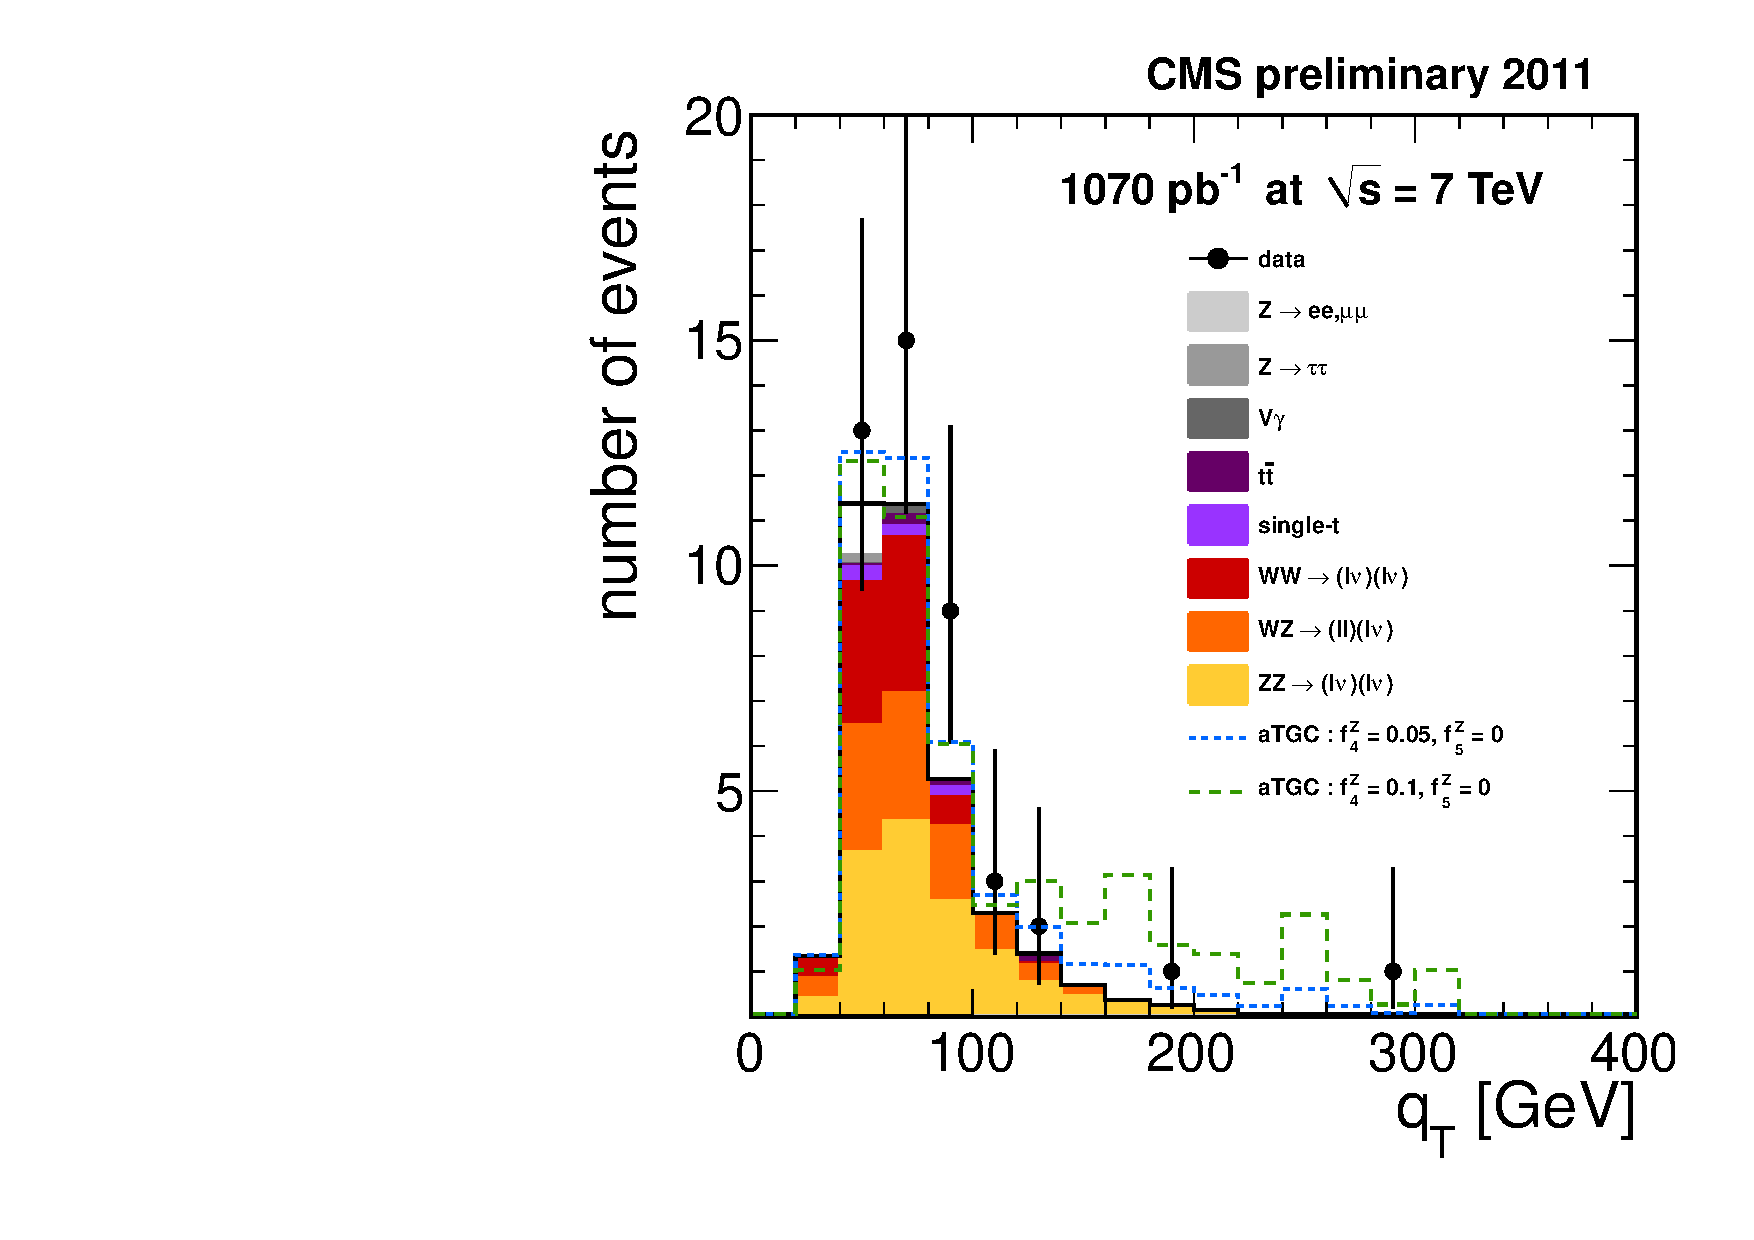
\includegraphics[width=1\textwidth]{figures/ZZ_2l2n/ZPtWithATGCs.pdf}
    \caption{ Transverse momentum of the \PZ\ boson after all selections, with examples of predictions with anomalous couplings. 
      \label{fig:ZZZaTGC_ZPt}}
\end{minipage}
\hspace{0.5cm}
\begin{minipage}[t]{0.48\linewidth}
\centering
    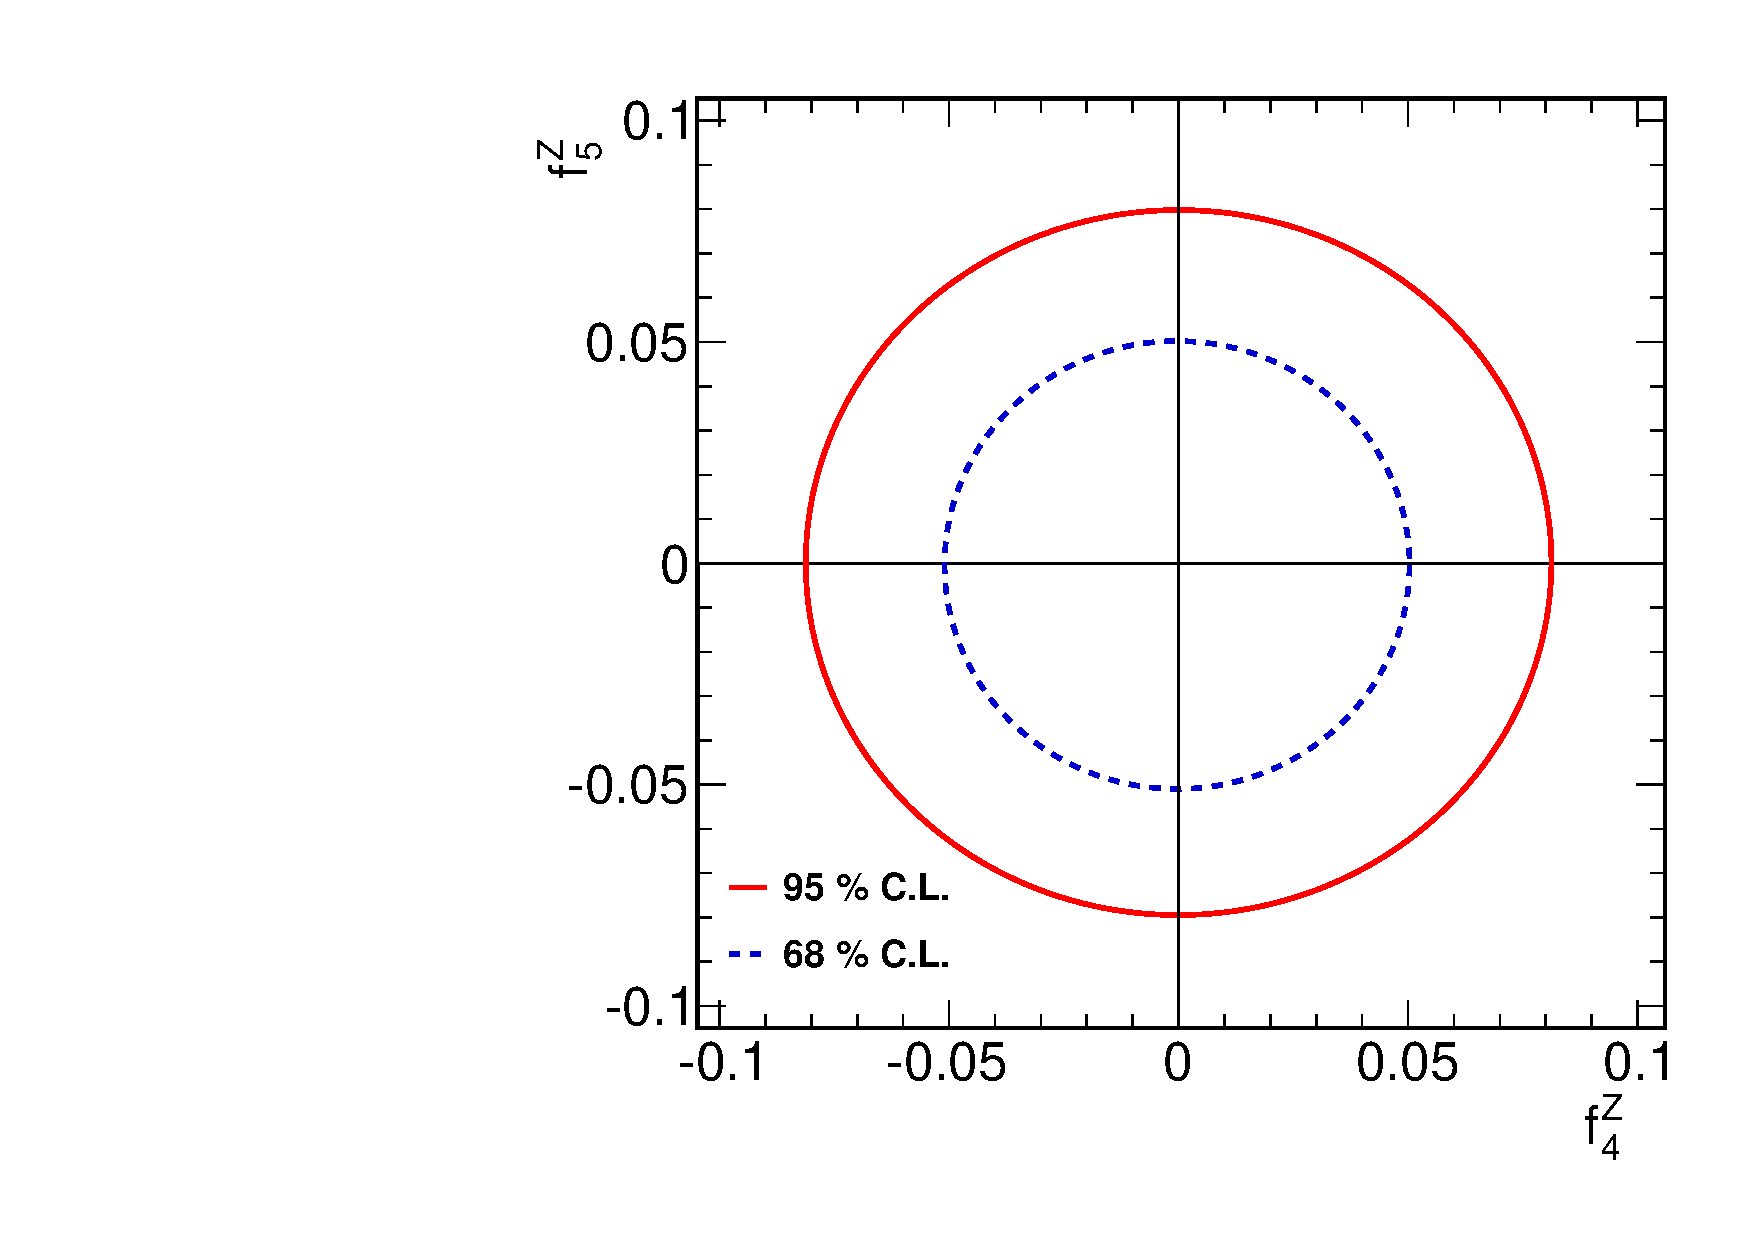
\includegraphics[width=0.95\textwidth]{figures/ZZ_2l2n/ZZZaTGC.pdf}
    \caption{ Two-dimensional limits on the $f_{4}^{\PZ}$ and $f_{5}^{\PZ}$ anomalous couplings.
      \label{fig:ZZZaTGC_2D}}
\end{minipage}
\end{figure}


%%%%%%%%%%%%%%%%%%%%%%%%%%%%%%%%%%%%%%%%%%%%%%%%%%%%%%%%%%%%%%%%%%%%%%%%%%

% >> acknowledgements (for journal papers)
% Please include the latest version from https://twiki.cern.ch/twiki/bin/viewauth/CMS/Internal/PubAcknow.
%\section*{Acknowledgements}
% ack-text

%% **DO NOT REMOVE BIBLIOGRAPHY**
%\newpage
\bibliography{auto_generated}   % will be created by the tdr script.

%% examples of appendices. **DO NOT PUT \end{document} at the end
%\clearpage
%\appendix

%%% DO NOT ADD \end{document}!

